% Arquivo LaTeX de exemplo de dissertação/tese a ser apresentados à CPG do IME-USP
%
% Versão 6: Sex Nov  10 18:00:00 BRT 2017
%
% Criação: Jesús P. Mena-Chalco
% Revisão: Fabio Kon e Paulo Feofiloff
% Adaptação para UTF8, biblatex e outras melhorias: Nelson Lago


%%%%%%%%%%%%%%%%%%%%%%%%%%%%%%%%%%%%%%%%%%%%%%%%%%%%%%%%%%%%%%%%%%%%%%%%%%%%%%%%
%%%%%%%%%%%%%%%%%%%%%%%%%%%%%%% PREÂMBULO LaTeX %%%%%%%%%%%%%%%%%%%%%%%%%%%%%%%%
%%%%%%%%%%%%%%%%%%%%%%%%%%%%%%%%%%%%%%%%%%%%%%%%%%%%%%%%%%%%%%%%%%%%%%%%%%%%%%%%

% Este pacote gera avisos durante a compilação sobre comandos
% considerados obsoletos.
\RequirePackage[l2tabu, orthodox]{nag}

% "Book" tem capítulos (e partes, mas normalmente não usamos) e, se o documento
% é frente-e-verso, cada capítulo começa em uma página de numeração ímpar.
% Report é similar, mas cada capítulo começa em uma nova página, par ou ímpar.
% É possível mudar esse comportamento com a opção "openany". Observe que você
% pode adaptar este modelo para escrever artigos, mudando a classe do
% documento de "book" para "article" ou a classe de algum periódico específico.
%
% A opção frente-e-verso aqui significa, por exemplo, que as margens das páginas
% ímpares e pares são diferentes ou que números de página aparecem à direita
% ou à esquerda alternadamente. Nada impede que você crie um documento "só
% frente" e, ao imprimir, faça a impressão frente-e-verso.
%
% Aqui também definimos a língua padrão do documento e línguas adicionais. A
% classe em si não usa essa informação mas, passando as opções de língua aqui,
% elas são repassadas para todas as packages, e diversas packages mudam
% seu comportamento em função da língua (em especial, babel/polyglossia).
% A última língua da lista é a língua padrão do documento.
%\documentclass[12pt,twoside,brazil,english]{book}
\documentclass[12pt,twoside,english,brazil]{book}
%\documentclass[12pt,twoside,english,brazil]{article}

% tamanho da página e margens
\usepackage[a4paper]{geometry}
\geometry{
  % distância entre o início da página e o início do texto principal
  top=32mm,
  bottom=28mm,
  left=24mm,
  right=34mm,
  % Com geometry, esta medida não é tão relevante; basta garantir que ela
  % seja menor que "top" e que o texto do cabeçalho caiba nela.
  headheight=25.4mm,
  % distância entre o início do texto principal e a base do cabeçalho;
  % ou seja, o cabeçalho "invade" a margem superior nessa medida. Essa
  % é a medida que determina a posição do cabeçalho
  headsep=11mm,
  footskip=10mm,
  marginpar=20mm,
  marginparsep=5mm,
}

% Vários pacotes e opções de configuração genéricos; para personalizar o
% resultado, modifique este arquivo.
%%%%%%%%%%%%%%%%%%%%%%%%%%%%%%%%%%%%%%%%%%%%%%%%%%%%%%%%%%%%%%%%%%%%%%%%%%%%%%%%
%%%%%%%%%%%%%%%%%%%%%%% CONFIGURAÇÕES E PACOTES BÁSICOS %%%%%%%%%%%%%%%%%%%%%%%%
%%%%%%%%%%%%%%%%%%%%%%%%%%%%%%%%%%%%%%%%%%%%%%%%%%%%%%%%%%%%%%%%%%%%%%%%%%%%%%%%

% Vários comandos auxiliares para o desenvolvimento de packages e classes;
% aqui, usamos em alguns comandos de formatação.
\usepackage{etoolbox}

% Detecta o tipo de sistema que estamos usando (XeTeX, LuaTeX ou pdfTeX). Na
% verdade, ifpdf não detecta pdfTeX, mas sim se estamos gerando um PDF; como
% só XeTeX, LuaTeX e pdfTeX geram PDFs, combinando todos é possível identificar
% pdfTeX também.
\usepackage{ifxetex}
\usepackage{ifluatex}
\usepackage{ifpdf}

% "fontenc" é um parâmetro interno do LaTeX. O fontenc default é OT1, mas ele
% tem algumas limitações; a mais importante é que, com ele, palavras acentuadas
% não podem ser hifenizadas. Por conta disso, quase todos os documentos LaTeX
% utilizam o fontenc T1. A escolha do fontenc tem consequências para as fontes
% que podem ser usadas no documento; hoje em dia T1 tem mais opções de
% qualidade, então não se perde nada.
\usepackage[T1]{fontenc}

% apenas útil para LaTeX tradicional e pdfTeX; XeTeX e LuaTeX usam sempre utf8.
\usepackage[utf8]{inputenc}

% Permite criar "headed lists", ou seja, "listas" de elementos que vão
% aparecendo ao longo do documento (como, por exemplo, teoremas). Podem ser
% também citações a autores específicos, seções de um documento que está
% sendo analisado etc. Precisa ser carregado antes das definições de fontes.
\usepackage{amsthm}

% Internacionalização dos nomes das seções ("chapter" X "capítulo" etc.),
% hifenização e outras convenções tipográficas. babel deve ser um dos
% primeiros pacotes carregados. É possível passar a língua do documento
% como parâmetro aqui, mas já fizemos isso ao carregar a classe, mais acima.
\usepackage{babel}

% Comandos rápidos para mudar de língua:
% \en -> muda para o inglês
% \br -> muda para o português
% \texten{blah} -> o texto "blah" é em inglês
% \textbr{blah} -> o texto "blah" é em português
\babeltags{br = brazil, en = english}

% É possível personalizar as palavras-chave que babel utiliza, por exemplo:
%\addto\extrasbrazil{\renewcommand{\refname}{Bibliografia}}

% Para línguas baseadas no alfabeto latino, como o inglês e o português,
% o pacote babel funciona muito bem, mas com outros alfabetos ele às vezes
% falha. Por conta disso, o pacote polyglossia foi criado para substituí-lo.
% polyglossia só funciona com LuaTeX e XeTeX; como babel também funciona com
% esses sistemas, provavelmente não há razão para usar polyglossia, mas é
% possível que no futuro esse pacote se torne o padrão.
%\usepackage{polyglossia}
%\setdefaultlanguage{brazil}
%\setotherlanguage{english}

% microajustes no tamanho das letras, espaçamento etc. para melhorar
% a qualidade visual do resultado. LaTeX tradicional não dá suporte a
% nenhum tipo de microajuste; pdfLaTeX dá suporte a todos. LuaLaTeX
% e XeLaTeX dão suporte a alguns:
%
% * expansion não funciona com XeLaTeX
% * tracking não funciona com XeLaTeX; é possível obter o mesmo resultado
%   com a opção "LetterSpace" do pacote fontspec, mas a configuração é
%   totalmente manual. Por padrão, aumenta o afastamento entre caracteres
%   nas fontes "small caps"; o resultado não se presta ao uso na
%   bibliografia ou citações, então melhor desabilitar.
% * kerning e spacing só funcionam com pdfLaTex; ambas são funções
%   consideradas experimentais e nem sempre produzem resultados vantajosos.

\newcommand\microtypeopts{
  protrusion=true,
  tracking=false,
  kerning=false,
  spacing=false
}

\ifxetex
  \usepackage[expansion=false,\microtypeopts]{microtype}
\else
  \usepackage[expansion=true,\microtypeopts]{microtype}
\fi

% Alguns "truques" (sujos?) para minimizar over/underfull boxes.
\tolerance=800
\hyphenpenalty=800
\setlength{\emergencystretch}{2.5em}

% Normalmente, LaTeX faz o final da página terminar sempre no mesmo lugar
% (exceto no final dos capítulos). Esse padrão pode ser ativado explicitamente
% com o comando "\flushbottom". Mas se, por alguma razão, o volume de texto na
% página é "pequeno", essa página vai ter espaços verticais artificialmente
% grandes. Uma solução para esse problema é modificar o padrão para
% "\raggedbottom"; isso permite que as páginas terminem em lugares diferentes.
% Outra opção é corrigir manualmente cada página problemática, por exemplo
% com o comando "\enlargethispage".
%\raggedbottom

% Por padrão, LaTeX coloca uma espaço aumentado após sinais de pontuação;
% Isso não é tão bom quanto alguns TeX-eiros defendem :) .
% Esta opção desabilita isso e, consequentemente, evita problemas com
% "id est" (i.e.) e "exempli gratia" (e.g.)
\frenchspacing

% LaTeX por default segue o estilo americano e não faz a indentação da
% primeira linha do primeiro parágrafo de uma seção; este pacote ativa essa
% indentação, como é o estilo brasileiro
\usepackage{indentfirst}

% LaTeX às vezes coloca notas de rodapé logo após o final do texto da
% página ao invés de no final da página; este pacote evita isso.
\usepackage[bottom]{footmisc}

% Se uma página está vazia, não imprime número de página ou cabeçalho
\usepackage{emptypage}

% Espaçamento entre linhas configurável (\singlespacing, \onehalfspacing etc.)
\usepackage{setspace}

% A primeira linha de cada parágrafo costuma ter um pequeno recuo para
% tornar mais fácil visualizar onde cada parágrafo começa. Além disso, é
% possível colocar um espaço em branco entre um parágrafo e outro. Esta
% package coloca o espaço em branco e desabilita o recuo; como queremos
% o espaço *e* o recuo, é preciso guardar o valor padrão do recuo e
% redefini-lo depois de carregar a package.
\newlength\oldparindent
\setlength\oldparindent\parindent
\usepackage[parfill]{parskip}
\setlength\parindent\oldparindent

% Carrega nomes de cores disponíveis (podem ser usados com hyperref e listings)
\usepackage[usenames,svgnames,dvipsnames]{xcolor}

% Por padrão, o algoritmo LaTeX para textos não-justificados é (muito) ruim;
% este pacote implementa um algoritmo bem melhor
\usepackage[newcommands]{ragged2e}

% Com ragged2e e a opção "newcommands", textos curtos não-justificados
% podem gerar warnings sobre "underfull \hbox". Não há razão para pensar
% muito nesses warnings, então melhor desabilitá-los.
% https://tex.stackexchange.com/questions/17659/ragged2e-newcommands-option-produces-underfull-hbox-warnings
\makeatletter
\g@addto@macro{\centering}{\hbadness=\@M}
\g@addto@macro{\Centering}{\hbadness=\@M}
\g@addto@macro{\raggedright}{\hbadness=\@M}
\g@addto@macro{\RaggedRight}{\hbadness=\@M}
\g@addto@macro{\raggedleft}{\hbadness=\@M}
\g@addto@macro{\RaggedLeft}{\hbadness=\@M}
\g@addto@macro{\center}{\hbadness=\@M}
\g@addto@macro{\Center}{\hbadness=\@M}
\g@addto@macro{\flushleft}{\hbadness=\@M}
\g@addto@macro{\FlushLeft}{\hbadness=\@M}
\g@addto@macro{\flushright}{\hbadness=\@M}
\g@addto@macro{\FlushRight}{\hbadness=\@M}
\makeatother

% LaTeX define os comandos "MakeUppercase" e "MakeLowercase", mas eles têm
% algumas limitações; esta package define os comandos MakeTextUppercase e
% MakeTextLowercase que resolvem isso.
\usepackage{textcase}


%%%%%%%%%%%%%%%%%%%%%%%%%%%%%%%%%%%%%%%%%%%%%%%%%%%%%%%%%%%%%%%%%%%%%%%%%%%%%%%%
%%%%%%%%%%%%%%%%%%%%%%%%%%%%%%%%%%% FONTE %%%%%%%%%%%%%%%%%%%%%%%%%%%%%%%%%%%%%%
%%%%%%%%%%%%%%%%%%%%%%%%%%%%%%%%%%%%%%%%%%%%%%%%%%%%%%%%%%%%%%%%%%%%%%%%%%%%%%%%

% LaTeX normalmente usa quatro tipos de fonte:
%
% * uma fonte serifada, para o corpo do texto;
% * uma fonte com design similar à anterior para modo matemático;
% * uma fonte sem serifa, para títulos ou "entidades". Por exemplo, "a classe
%   \textsf{TimeManager} é responsável..." ou "chamamos \textsf{primos} os
%   números que...". Observe que em quase todos os casos desse tipo é mais
%   adequado usar negrito ou itálico;
% * uma fonte "teletype", para trechos de programas.
%
% A escolha de uma família de fontes para o documento por default seleciona as
% quatro fontes de uma vez.
%
% LaTeX usa por default a família de fontes "Computer Modern". Essas fontes
% precisaram ser re-criadas diversas vezes em formatos diferentes, então há
% diversas variantes dela. Com o fontenc OT1 (default "ruim" do LaTeX), a
% versão usada é a BlueSky Computer Modern, que é de boa qualidade, mas com os
% problemas do OT1. Com fontenc T1 (padrão deste modelo e recomendado), o
% LaTeX usa o conjunto "cm-super". Essa versão das fontes tem vantagens e
% desvantagens; em particular, às vezes o sistema usa fontes bitmap, que são
% ruins para leitura na tela. Ao longo do tempo, versões diferentes dessas
% fontes foram recomendadas como "a melhor"; atualmente, a melhor opção para
% usar a família Computer Modern é a versão "Latin Modern".
\usepackage{lmodern}

% Latin Modern não tem fontes bold + Small Caps, mas cm-super sim;
% assim, vamos ativar o suporte às fontes cm-super (sem ativá-las
% como a fonte padrão do documento) e configurar substituições
% automáticas para que a fonte Latin Modern seja substituída por
% cm-super quando o texto for bold + Small Caps.
\usepackage{fix-cm}

% É preciso incluir substituições para o encoding TS1 também por conta
% dos números oldstyle, porque para inclui-los nas fontes computer modern
% foi feita uma hack: os dígitos são declarados como sendo os números
% itálicos da fonte matemática e, portanto, estão no encoding TS1.
%
% Primeiro forçamos o LaTeX a carregar a fonte Latin Modern (ou seja, ler
% o arquivo que inclui "DeclareFontFamily") e, a seguir, definimos a
% substituição
\fontencoding{TS1}\fontfamily{lmr}\selectfont
\DeclareFontShape{TS1}{lmr}{b}{sc}{<->ssub * cmr/bx/n}{}
\DeclareFontShape{TS1}{lmr}{bx}{sc}{<->ssub * cmr/bx/n}{}

\fontencoding{T1}\fontfamily{lmr}\selectfont
\DeclareFontShape{T1}{lmr}{b}{sc}{<->ssub * cmr/bx/sc}{}
\DeclareFontShape{T1}{lmr}{bx}{sc}{<->ssub * cmr/bx/sc}{}

% Latin Modern não tem "small caps + itálico", mas tem "small caps + slanted";
% vamos definir mais uma substituição aqui.
\fontencoding{T1}\fontfamily{lmr}\selectfont % já feito acima, mas tudo bem
\DeclareFontShape{T1}{lmr}{m}{scit}{<->ssub * lmr/m/scsl}{}
\DeclareFontShape{T1}{lmr}{bx}{scit}{<->ssub * lmr/bx/scsl}{}

% Se fizermos mudanças manuais na fonte, estes comandos podem vir
% a ser úteis
%\newcommand\lmodern{%
%  \renewcommand{\oldstylenums}[1]{{\fontencoding{TS1}\selectfont ##1}}%
%  \fontfamily{lmr}\selectfont%
%}
%
%\DeclareRobustCommand\textlmodern[1]{%
%  {\lmodern #1}%
%}

% É possível mudar apenas uma das fontes. Em particular, a fonte
% teletype da família Computer Modern foi criada para simular
% as impressoras dos anos 1970/1980. Sendo assim, ela é uma fonte (1)
% com serifas e (2) de espaçamento fixo. Hoje em dia, é mais comum usar
% fontes sem serifa para representar código-fonte. Além disso, ao imprimir,
% é comum adotar fontes que não são de espaçamento fixo para fazer caber
% mais caracteres em uma linha de texto. Algumas opções de fontes para
% esse fim:
%\usepackage{newtxtt}
%\usepackage{DejaVuSansMono}
\usepackage{inconsolata}

% Ao invés da família Computer Modern, é possível usar outras como padrão.
% Uma ótima opção é a libertine, similar (mas não igual) à Times mas com
% suporte a Small Caps e outras qualidades. A fonte teletype da família
% é serifada, então é melhor definir outra; a opção "mono=false" faz
% o pacote não carregar sua própria fonte, mantendo a escolha anterior.
% A opção "nofontspec" elimina um problema de compatibilidade com algumas
% outras fontes; remova-a se você for utilizar XeLaTeX ou a package fontspec,
% mais abaixo.
\usepackage[mono=false,nofontspec]{libertine}
% A família libertine por padrão não define uma fonte matemática específica;
% uma opção que funciona bem com ela:
\usepackage[libertine]{newtxmath}
% Ativa apenas a fonte biolinum, que é a fonte sem serifa da família.
%\usepackage[nofontspec]{biolinum}

% Também é possível usar a Times como padrão; nesse caso, a fonte sem serifa
% é a Helvetica. Mas provavelmente libertine é uma opção melhor.
%\usepackage[helvratio=0.95,largesc]{newtxtext}

% gentium inclui apenas uma fonte serifada, similar a Garamond, que busca
% cobrir todos os caracteres unicode
%\usepackage{gentium}

% LaTeX normalmente funciona com fontes que foram adaptadas para ele, ou
% seja, ele não usa as fontes padrão instaladas no sistema: para usar
% uma fonte é preciso ativar o pacote correspondente, como visto acima.
% É possível escapar dessa limitação e acessar as fontes padrão do sistema
% com XeTeX ou LuaTeX. Com eles, além dos pacotes de fontes "tradicionais",
% pode-se usar o pacote fontspec para usar fontes do sistema.
%\usepackage{fontspec}
%\setmainfont{DejaVu Serif}
%\setmainfont{Charis SIL}
%\setsansfont{DejaVu Sans}
%\setsansfont{Libertinus Sans}[Scale=1.1]
%\setmonofont{DejaVu Sans Mono}

% fontspec oferece vários recursos interessantes para manipular fontes.
% Por exemplo, Garamond é uma fonte clássica; a versão EBGaramond é muito
% boa, mas não possui versões bold e bold-italic; aqui, usamos
% CormorantGaramond ou Gentium para simular a versão bold.
%\setmainfont{EBGaramond12}[
%  Numbers        = {Lining,} ,
%  Scale          = MatchLowercase ,
%  UprightFont    = *-Regular ,
%  ItalicFont     = *-Italic ,
%  BoldFont       = gentiumbasic-bold ,
%  BoldItalicFont = gentiumbasic-bolditalic ,
%%  BoldFont       = CormorantGaramond Bold ,
%%  BoldItalicFont = CormorantGaramond Bold Italic ,
%]
%
%\newfontfamily\garamond{EBGaramond12}[
%  Numbers        = {Lining,} ,
%  Scale          = MatchLowercase ,
%  UprightFont    = *-Regular ,
%  ItalicFont     = *-Italic ,
%  BoldFont       = gentiumbasic-bold ,
%  BoldItalicFont = gentiumbasic-bolditalic ,
%%  BoldFont       = CormorantGaramond Bold ,
%%  BoldItalicFont = CormorantGaramond Bold Italic ,
%]

% Crimson tem Small Caps, mas o recurso é considerado "em construção".
% Vamos utilizar Gentium para Small Caps
%\setmainfont{Crimson}[
%  Numbers           = {Lining,} ,
%  Scale             = MatchLowercase ,
%  UprightFont       = *-Roman ,
%  ItalicFont        = *-Italic ,
%  BoldFont          = *-Bold ,
%  BoldItalicFont    = *-Bold Italic ,
%  SmallCapsFont     = Gentium Plus ,
%  SmallCapsFeatures = {Letters=SmallCaps} ,
%]
%
%\newfontfamily\crimson{Crimson}[
%  Numbers           = {Lining,} ,
%  Scale             = MatchLowercase ,
%  UprightFont       = *-Roman ,
%  ItalicFont        = *-Italic ,
%  BoldFont          = *-Bold ,
%  BoldItalicFont    = *-Bold Italic ,
%  SmallCapsFont     = Gentium Plus ,
%  SmallCapsFeatures = {Letters=SmallCaps} ,
%]

% Com o pacote fontspec, também é possível usar o comando "\fontspec" para
% selecionar uma fonte temporariamente, sem alterar as fontes-padrão do
% documento.

% Tanto Small Caps quanto itálico (ou slanted) são "shapes" de uma fonte.
% Sendo assim, os comandos \scshape (ou \textsc) e \itshape (ou \textit) são
% "incompatíveis" entre si, ou seja, um cancela o outro. O que LaTeX faz é
% considerar que há um outro shape: "small caps + itálico" (ou "small caps +
% slanted"), chamado "scit" ou "scsl". Se a fonte oferece esse shape, é só
% usar \fontshape(scit}\selectfont. Mas isso é muito desconfortável, já que
% o usual seria algo como "\textsc{Algumas \textit{palavras} podem ser
% diferentes}". Esta package resolve esse problema.
\usepackage{slantsc}


%%%%%%%%%%%%%%%%%%%%%%%%%%%%%%%%%%%%%%%%%%%%%%%%%%%%%%%%%%%%%%%%%%%%%%%%%%%%%%%%
%%%%%%%%%%%%%%%%%%%%%%%%%%% APARÊNCIA/FORMATAÇÃO %%%%%%%%%%%%%%%%%%%%%%%%%%%%%%%
%%%%%%%%%%%%%%%%%%%%%%%%%%%%%%%%%%%%%%%%%%%%%%%%%%%%%%%%%%%%%%%%%%%%%%%%%%%%%%%%

% Formatação personalizada das listas "itemize", "enumerate" e
% "description", além de permitir criar novos tipos de listas
%\usepackage{paralist}

% Formatação personalizada do sumário, lista de tabelas/figuras etc.
%\usepackage{titletoc}

% Lembre-se que titlesec é incompatível com os comandos refsection
% e refsegment do pacote biblatex!
% Formatação personalizada de títulos, seções etc.
% Cabeçalhos dos títulos: negrito (bf), fonte um pouco menor (medium)
% e menos espaçamento vertical (compact)
%\usepackage[bf,medium,compact]{titlesec}

% Permite saber o número total de páginas; útil para colocar no
% rodapé algo como "página 3 de 10" com "\thepage de \pageref{LastPage}"
%\usepackage{lastpage}

% Formatação dos cabeçalhos e rodapés
\usepackage{fancyhdr}

% Sem linha separando o cabeçalho
\renewcommand{\headrulewidth}{0pt}

% A formatação dos cabeçalhos/rodapés envolve duas coisas:
% 1. Escolher qual texto deve ser impresso nas páginas pares/ímpares
%    (nome do capítulo ou seção, nome do autor etc.)
% 2. Escolher o lugar e a formatação desse texto e da numeração de páginas
%
% O lugar e a formatação são definidos com os comandos fancyhead e
% fancyfoot. "RO" significa "Right side of Odd pages"; "LE" significa
% "Left side of Even pages" etc.
%
% A escolha do texto é feita com os comandos chaptermark/sectionmark;
% os nomes "left/right/both" usados por esses comandos não fazem muito
% sentido, melhor pensar neles como palavras "mágicas". Para fazer
% mudanças não triviais aqui é necessário ler a documentação.
%
% O comando "\chaptermark\markboth" define o que fica guardado na variável
% "leftmark". Pode ser só "##1" (o nome do capítulo), pode ser
% "\thechapter. ##1" (aí inclui o número do capítulo), pode ser
% "\chaptername\ \thechapter. ##1" (aí inclui a palavra "capítulo") etc.
%
% O comando \sectionmark\markright" define o que fica guardado na variável
% "rightmark". Pode ser só "##1" (o nome da seção dentro do capítulo),
% pode ser "\thesection. ##1" (aí inclui o número da seção), pode ser
% "\sectionname\ \thesection. ##1" (aí inclui a palavra "seção") etc.

% Só olha até o nível 2 (seções), ou seja, não coloca nomes de
% subseções ou subsubseções nos cabeçalhos.
\setcounter{tocdepth}{2}

% Queremos colocar o número da página mais próximo da borda do papel (na
% horizontal). Para isso, vamos aumentar \headwidth, somando "tamanho da
% margem direita -10mm" (o número vai ficar a 10mm da borda).
%
% Observe que a package geometry define \evensidemargin, mas seu valor não
% necessariamente corresponde ao que queremos aqui (não sei bem como nem
% por que geometry define esse valor). Ao invés de usá-lo, vamos calcular
% manualmente.
%
% A distância entre a borda esquerda/interna do papel e o início do texto
% é dada por (1in + \hoffset + \oddsidemargin); a margem direita, portanto,
% é dada por (\paperwidth - (1in + \hoffset + \oddsidemargin + \textwidth)).
\dimdef{\othermargin}{\paperwidth - 1in - \hoffset - \oddsidemargin - \textwidth}
\addtolength{\headwidth}{\othermargin}
\addtolength{\headwidth}{-10mm}

\newcommand{\formataNumPaginas}{
  \fancyhead[RO]{\raisebox{8mm}{\footnotesize\bfseries\thepage}}
  \fancyhead[LE]{\raisebox{8mm}{\footnotesize\bfseries\thepage}}
}

\newcommand{\formataCabecalhosDinamicos}{
  \fancyhead[LO]{\scriptsize\MakeTextUppercase{\rightmark}}
  \fancyhead[RE]{\scriptsize\MakeTextUppercase{\leftmark}}
}

\fancypagestyle{mainmatter}{
  % Nome do capítulo no cabeçalho das páginas pares (e nas
  % ímpares quando não há seções)
  \renewcommand{\chaptermark}[1]{
    \markboth
      {\thechapter\hskip 0.3em |\hskip 0.3em ##1}
      {\thechapter\hskip 0.3em |\hskip 0.3em ##1}
  }

  % Número e nome da seção no cabeçalho das páginas ímpares
  \renewcommand{\sectionmark}[1]{
    \markright{\thesection\hskip 0.3em |\hskip 0.3em ##1}
  }

  \fancyhf{}
  \formataNumPaginas{}
  \formataCabecalhosDinamicos{}
}

\fancypagestyle{appendix}{
  \renewcommand{\chaptermark}[1]{%
    \markboth{%
      % Páginas ímpares: "Apêndice X"
      \appendixname\ \thechapter%
    }{%
      % Páginas pares: "X | nome do apêndice"
      \thechapter\hskip 0.3em |\hskip 0.3em ##1%
    }
  }

  \fancyhf{}
  \formataNumPaginas{}
  \formataCabecalhosDinamicos{}
}

% Na frontmatter e backmatter, não há números de capítulos e (em geral)
% não há subdivisões (capítulos/seções/subseções), apenas um nível.
% O correto, então, é usar o mesmo texto (nome do capítulo ou seção)
% nas páginas pares ou ímpares. Isso na verdade não está funcionando
% na frontmatter, pois os capítulos ali não definem os cabeçalhos (não
% executam "chaptermark/sectionmark"), mas "forçamos" a bibliografia
% e o índice a usarem.
\fancypagestyle{frontback}{
  \renewcommand{\chaptermark}[1]{\markboth{##1}{##1}}
  \renewcommand{\sectionmark}[1]{\markboth{##1}{##1}}

  \fancyhf{}
  \formataNumPaginas{}
  \formataCabecalhosDinamicos{}
}

% A página inicial de cada capítulo é automaticamente configurada para o estilo
% "plain", então vamos definir esse estilo (colocando o número de página no
% mesmo lugar das demais). As páginas iniciais também usam esse estilo.
\fancypagestyle{plain}{
  \fancyhf{}
  \formataNumPaginas{}
}


%%%%%%%%%%%%%%%%%%%%%%%%%%%%%%%%%%%%%%%%%%%%%%%%%%%%%%%%%%%%%%%%%%%%%%%%%%%%%%%%
%%%%%%%%%%%%%%%%%%%%%%%%%%%%% FIGURAS / FLOATS %%%%%%%%%%%%%%%%%%%%%%%%%%%%%%%%%
%%%%%%%%%%%%%%%%%%%%%%%%%%%%%%%%%%%%%%%%%%%%%%%%%%%%%%%%%%%%%%%%%%%%%%%%%%%%%%%%

% Permite importar figuras. LaTeX "tradicional" só é capaz de trabalhar com
% figuras EPS. Hoje em dia não há nenhuma boa razão para usar essa versão;
% pdfTeX, XeTeX, e LuaTeX podem usar figuras nos formatos PDF, JPG e PNG; EPS
% também pode funcionar em algumas instalações mas não é garantido, então é
% melhor evitar.
\usepackage{graphicx}

% Diretório onde estão as figuras; com isso, não é preciso colocar o caminho
% completo em \includegraphics. Na verdade, não precisa nem colocar a extensão
\graphicspath{{./figuras/}}

% Mais tipos de float e mais opções para personalização; este pacote
% também acrescenta a possibilidade de definir "H" como opção de
% posicionamento do float, que significa "aqui, incondicionalmente".
\usepackage{float}

% Por padrão, LaTeX prefere colocar floats no topo da página que
% onde eles foram definidos; vamos mudar isso. Este comando depende
% do pacote "float", carregado logo acima.
\floatplacement{table}{htbp}
\floatplacement{figure}{htbp}

% Garante que floats (tabelas e figuras) só apareçam após as seções a que
% pertencem. Por padrão, se a seção começa no meio da página, LaTeX pode
% colocar a figura no topo dessa página
\usepackage{flafter}
% Às vezes um float pode ser adiado por muitas páginas; é possível forçar
% LaTeX a imprimir todos os floats pendentes com o comando \clearpage.
% Esta package acrescenta o comando \FloatBarrier, que garante que floats
% definidos anteriormente sejam impressos e garante que floats subsequentes
% não apareçam antes desse ponto. A opção "section" faz o comando ser
% aplicado automaticamente a cada nova seção. "above" e "below" desabilitam
% a barreira quando os floats estão na mesma página.
\usepackage[section,above,below]{placeins}

% LaTeX escolhe automaticamente o "melhor" lugar para colocar cada float.
% Por padrão, ele tenta colocá-los no topo da página e depois no pé da
% página; se não tiver sucesso, vai para a página seguinte e recomeça.
% Se esse algoritmo não tiver sucesso "logo", LaTeX cria uma página só
% com floats. É possível modificar esse comportamento com as opções de
% posicionamento: "tp", por exemplo, instrui LaTeX a não colocar floats
% no pé da página, e "htbp" o instrui para tentar "aqui" como a primeira
% opção. O pacote "float" acrescenta a opção "H", que significa "aqui,
% incondicionalmente".
%
% A escolha do "melhor" lugar leva em conta os parâmetros abaixo, mas é
% possível ignorá-los com a opção de posicionamento "!". Dado que os
% valores default não são muito bons para floats "grandes" ou documentos
% com muitos floats, é muito comum usar "!" ou "H". No entanto, modificando
% esses parâmetros o algoritmo automático tende a funcionar bem.

% Fração da página que pode ser ocupada por floats no topo. Default: 0.7
\renewcommand{\topfraction}{.85}
% Idem para documentos em colunas e floats que tomam as 2 colunas. Default: 0.7
\renewcommand{\dbltopfraction}{.66}
% Fração da página que pode ser ocupada por floats no pé. Default: 0.3
\renewcommand{\bottomfraction}{.7}
% Fração mínima da página que deve conter texto. Default: 0.2
\renewcommand{\textfraction}{.15}
% Numa página só de floats, fração mínima que deve ser ocupada. Default: 0.5
\renewcommand{\floatpagefraction}{.66}
% Idem para documentos em colunas e floats que tomam as 2 colunas. Default: 0.5
\renewcommand{\dblfloatpagefraction}{.66}
% Máximo de floats no topo da página. Default: 2
\setcounter{topnumber}{9}
% Idem para documentos em colunas e floats que tomam as 2 colunas. Default: 2
\setcounter{dbltopnumber}{9}
% Máximo de floats no pé da página. Default: 1
\setcounter{bottomnumber}{9}
% Máximo de floats por página. Default: 3
\setcounter{totalnumber}{20}

% Define o ambiente "\begin{landscape} -- \end{landscape}"; o texto entre
% esses comandos é impresso em modo paisagem, podendo se estender por várias
% páginas. A rotação não inclui os cabeçalhos e rodapés das páginas.
% O principal uso desta package é em conjunto com a package longtable: se
% você precisa mostrar uma tabela muito larga (que precisa ser impressa em
% modo paisagem) e longa (que se estende por várias páginas), use
% "\begin{landscape}" e "\begin{longtable}" em conjunto. Note que o modo
% landscape entra em ação imediatamente, ou seja, "\begin{landscape}" gera
% uma quebra de página no local em que é chamado. Na maioria dos casos, o
% que se quer não é isso, mas sim um "float paisagem"; isso é o que a
% package rotating oferece (veja abaixo).
\usepackage{pdflscape}

% Define dois novos tipos de float: sidewaystable e sidewaysfigure, que
% imprimem a figura ou tabela sozinha em uma página em modo paisagem. Além
% disso, permite girar elementos na página de diversas outras maneiras.
\usepackage[figuresright,clockwise]{rotating}

% Captions com fonte menor, indentação normal, corpo do texto
% negrito e nome do caption itálico
\usepackage[
  font=small,
  format=plain,
  labelfont=bf,up,
  textfont=it,up]{caption}

% Sub-figuras (e seus captions) - observe que existe uma package chamada
% "subfigure", mas ela é obsoleta; use esta no seu lugar.
\usepackage{subcaption}

% Permite criar imagens com texto ao redor
\usepackage{wrapfig}

% Permite incorporar um arquivo PDF como uma página adicional. Útil se
% for necessário importar uma imagem ou tabela muito grande ou ainda
% para definir uma capa personalizada.
\usepackage{pdfpages}


%%%%%%%%%%%%%%%%%%%%%%%%%%%%%%%%%%%%%%%%%%%%%%%%%%%%%%%%%%%%%%%%%%%%%%%%%%%%%%%%
%%%%%%%%%%%%%%%%%%%%%%%%%%%%%%%%%% TABELAS %%%%%%%%%%%%%%%%%%%%%%%%%%%%%%%%%%%%%
%%%%%%%%%%%%%%%%%%%%%%%%%%%%%%%%%%%%%%%%%%%%%%%%%%%%%%%%%%%%%%%%%%%%%%%%%%%%%%%%

% Tabelas simples são fáceis de fazer em LaTeX; tabelas com alguma sofisticação
% são trabalhosas, pois é difícil controlar alinhamento, largura das colunas,
% distância entre células etc. Ou seja, é muito comum que a tabela final fique
% "torta". Por isso, em muitos casos, vale mais a pena gerar a tabela em uma
% planilha, como LibreOffice calc ou excel, transformar em PDF e importar como
% figura, especialmente se você quer controlar largura/altura das células
% manualmente etc. No entanto, se você quiser fazer as tabelas em LaTeX para
% garantir a consistência com o tipo e o tamanho das fontes, é possível e o
% resultado é muito bom. Aqui há alguns pacotes que incrementam os recursos de
% tabelas do LaTeX e alguns comandos pré-prontos que podem facilitar um pouco
% seu uso.

% LaTeX por padrão não permite notas de rodapé dentro de tabelas;
% este pacote acrescenta essa funcionalidade.
\usepackage{tablefootnote}

% Estende o ambiente tabular para que, além de "l", "c", "r" para definir se uma
% coluna deve ser alinhada à esquerda, centralizada ou à direita, seja possível
% definir a largura das colunas (além de outras pequenas modificações). Isso é
% muito útil porque LaTeX não "percebe" automaticamente quando é mais
% interessante fazer uma coluna mais estreita e forçar quebras de linha nas
% células correspondentes.
\usepackage{array}

% Se você quer ter um pouco mais de controle sobre o tamanho de cada coluna da
% tabela, utilize estes tipos de coluna (criados com base nos recursos do pacote
% array). É só usar algo como M{número}, onde "número" (por exemplo, 0.4) é a
% fração de \textwidth que aquela coluna deve ocupar. "M" significa que o
% conteúdo da célula é centralizado; "L", alinhado à esquerda; "J", justificado;
% "R", alinhado à direita. Obviamente, a soma de todas as frações não pode ser
% maior que 1, senão a tabela vai ultrapassar a linha da margem.
\newcolumntype{M}[1]{>{\centering}m{#1\textwidth}}
\newcolumntype{L}[1]{>{\RaggedRight}m{#1\textwidth}}
\newcolumntype{R}[1]{>{\RaggedLeft}m{#1\textwidth}}
\newcolumntype{J}[1]{m{#1\textwidth}}

% Permite alinhar os elementos de uma coluna pelo ponto decimal
\usepackage{dcolumn}

% Define tabelas do tipo "longtable", similares a "tabular" mas que podem ser
% divididas em várias páginas. "longtable" também funciona corretamente com
% notas de rodapé. Note que, como uma longtable pode se estender por várias
% páginas, não faz sentido colocá-las em um float "table". Por conta disso,
% longtable define o comando "\caption" internamente.
\usepackage{longtable}

% Permite agregar linhas de tabelas, fazendo colunas "compridas"
\usepackage{multirow}

% Cria comando adicional para possibilitar a inserção de quebras de linha
% em uma célula de tabela, entre outros
\usepackage{makecell}

% Às vezes a tabela é muito larga e não cabe na página. Se os cabeçalhos da
% tabela é que são demasiadamente largos, uma solução é inclinar o texto das
% células do cabeçalho. Para fazer isso, use o comando "\rothead".
\renewcommand{\rothead}[2][60]{\makebox[11mm][l]{\rotatebox{#1}{\makecell[c]{#2}}}}

% Se quiser criar uma linha mais grossa no meio de uma tabela, use
% o comando "\thickhline".
\newlength\savedwidth
\newcommand\thickhline{
  \noalign{
    \global\savedwidth\arrayrulewidth
    \global\arrayrulewidth 1.5pt
  }
  \hline
  \noalign{\global\arrayrulewidth\savedwidth}
}

% Modifica (melhora) o layout default das tabelas e acrescenta os comandos
% \toprule, \bottomrule, \midrule e \cmidrule
\usepackage{booktabs}

%%%%%%%%%%%%%%%%%%%%%%%%%%%%%%%%%%%%%%%%%%%%%%%%%%%%%%%%%%%%%%%%%%%%%%%%%%%%%%%%
%%%%%%%%%%%%%%%%%%%%%%%%%%%%%%%%% ESTRUTURA %%%%%%%%%%%%%%%%%%%%%%%%%%%%%%%%%%%%
%%%%%%%%%%%%%%%%%%%%%%%%%%%%%%%%%%%%%%%%%%%%%%%%%%%%%%%%%%%%%%%%%%%%%%%%%%%%%%%%

% acrescentamos a bibliografia/indice/conteudo no Sumário, mas excluímos as
% listas de figuras e tabelas e o próprio sumário.
\usepackage[nottoc,notlot,notlof]{tocbibind}

% Cria índice remissivo. Este pacote precisa ser carregado antes de hyperref.
% A criação do índice remissivo depende de um programa auxiliar, que pode ser
% o "makeindex" (default) ou o xindy. xindy é mais poderoso e lida melhor com
% línguas diferentes e caracteres acentuados, mas índices criados com xindy não
% funcionam em conjunto com hyperref. Para contornar esse problema,
% configuramos hyperref para *não* gerar hyperlinks no índice (mais abaixo)
% e configuramos xindy para que ele gere esses hyperlinks por conta própria.
% Se preferir usar makeindex, modifique a chamada ao pacote imakeidx (aqui)
% e altere as opções do pacote hyperref.

% Cria o arquivo de configuração para xindy lidar corretamente com hyperlinks.
\begin{filecontents*}{hyperxindy.xdy}
(define-attributes ("emph"))
(markup-locref :open "\hyperpage{" :close "}" :attr "default")
(markup-locref :open "\textbf{\hyperpage{" :close "}}" :attr "textbf")
(markup-locref :open "\textit{\hyperpage{" :close "}}" :attr "textit")
(markup-locref :open "\emph{\hyperpage{" :close "}}" :attr "emph")
\end{filecontents*}

% Cria o arquivo de configuração para makeindex colocar um cabeçalho
% para cada letra do índice.
\begin{filecontents*}{mkidxhead.ist}
headings_flag 1
heading_prefix "{\\bfseries "
heading_suffix "}\\nopagebreak\n"
\end{filecontents*}

%\usepackage[xindy]{imakeidx} % usando xindy
\usepackage{imakeidx} % usando makeindex

% Por padrão, o cabeçalho das páginas do índice é feito em maiúsculas;
% vamos mudar isso e deixar fancyhdr definir a formatação
\indexsetup{
  othercode={\chaptermark{\indexname}},
}

\makeindex[
  noautomatic,
  intoc,
  % Estas opções são usadas por xindy
  % "-C utf8" ou "-M lang/latin/utf8.xdy" são truques para contornar este
  % bug, que existe em outras distribuições tambem:
  % https://bugs.launchpad.net/ubuntu/+source/xindy/+bug/1735439
  % Se "-C utf8" não funcionar, tente "-M lang/latin/utf8.xdy"
  %options=-C utf8 -M hyperxindy.xdy,
  %options=-M lang/latin/utf8.xdy -M hyperxindy.xdy,
  % Estas opções são usadas por makeindex
  options=-s mkidxhead.ist -l -L,
]


%%%%%%%%%%%%%%%%%%%%%%%%%%%%%%%%%%%%%%%%%%%%%%%%%%%%%%%%%%%%%%%%%%%%%%%%%%%%%%%%
%%%%%%%%%%%%%%%%%%%%%%%%%%%% OUTROS PACOTES ÚTEIS %%%%%%%%%%%%%%%%%%%%%%%%%%%%%%
%%%%%%%%%%%%%%%%%%%%%%%%%%%%%%%%%%%%%%%%%%%%%%%%%%%%%%%%%%%%%%%%%%%%%%%%%%%%%%%%

% Você provavelmente vai querer ler a documentação de alguns destes pacotes
% para personalizar algum aspecto do trabalho ou usar algum recurso específico.

% Trechos de texto "puro" (tabs, quebras de linha etc. não são modificados)
\usepackage{verbatim}

% Recursos adicionais para o modo matemático
% para evitar problemas de compatibilidade com algumas fontes, o pacote
% amsthm já foi carregado mais acima
\usepackage{latexsym}
\usepackage{amsmath}
\usepackage{commath} 
% \usepackage{amssymb}
\usepackage{mathtools}

% Notação bra-ket
%\usepackage{braket}

%\num \SI and \SIrange. For example, \SI{10}{\hertz} \SIrange{10}{100}{\hertz}
%\usepackage[binary-units]{siunitx}

% Citações melhores; se você pretende fazer citações de textos
% relativamente extensos, vale a pena ler a documentação. biblatex
% utiliza recursos deste pacote.
\usepackage{csquotes}

% O comando \ref por padrão mostra apenas o número do elemento a que se
% refere; assim, é preciso escrever "veja a Figura \ref{grafico}" ou
% "como visto na Seção \ref{sec:introducao}". Usando o pacote hyperref
% (carregado mais abaixo), esse número é transformado em um hiperlink.
%
% Se você quiser mudar esse comportamento, ative as packages varioref
% e cleveref e também as linhas "labelformat" e "crefname" mais abaixo.
% Nesse caso, você deve escrever apenas "veja a \ref{grafico}" ou
% "como visto na \ref{sec:introducao}" etc. e o nome do elemento será
% gerado automaticamente como hiperlink.
%
% Se, além dessa mudança, você quiser usar os recursos de varioref ou
% cleveref, mantenha as linhas labelformat comentadas e use os comandos
% \vref ou \cref, conforme sua preferência, também sem indicar o nome do
% elemento, que é inserido automaticamente. Vale lembrar que o comando
% \vref de varioref pode causar problemas com hyperref, impedindo a
% geração do PDF final.
%
% ATENÇÃO: varioref, hyperref e cleveref devem ser carregadas nessa ordem!
%\usepackage{varioref}

%\labelformat{figure}{Figura~#1}
%\labelformat{table}{Tabela~#1}
%\labelformat{equation}{Equação~#1}
%% Isto não funciona corretamente com os apêndices; o comando seguinte
%% contorna esse problema
%%\labelformat{chapter}{Capítulo~#1}
%\makeatletter
%\labelformat{chapter}{\@chapapp~#1}
%\makeatother
%\labelformat{section}{Seção~#1}
%\labelformat{subsection}{Seção~#1}
%\labelformat{subsubsection}{Seção~#1}

% Cria hiperlinks para capítulos, seções, \ref's, URLs etc.
\usepackage[
  unicode=true,
  plainpages=false,
  pdfpagelabels,
  colorlinks=true,
  %citecolor=black,
  %linkcolor=black,
  %urlcolor=black,
  %filecolor=black,
  citecolor=DarkGreen,
  linkcolor=NavyBlue,
  urlcolor=DarkRed,
  filecolor=green,
  bookmarksopen=true,
  % hyperref não gera hyperlinks corretos em índices remissivos criados com
  % xindy; assim, desabilitamos essa função aqui e geramos os hyperlinks
  % com uma configuração especial de xindy (mais acima). Se você preferir
  % usar makeindex, (removendo a opção "xindy" do pacote imakeidx), quem
  % precisa criar os hyperlinks é hyperref. Nesse caso, desabilite a
  % próxima linha para criar hyperlinks no índice.
  %hyperindex=false,
]{hyperref}

%\usepackage[nameinlink,noabbrev,capitalise]{cleveref}
%% cleveref não tem tradução para o português
%\crefname{figure}{Figura}{Figuras}
%\crefname{table}{Tabela}{Tabelas}
%\crefname{chapter}{Capítulo}{Capítulos}
%\crefname{section}{Seção}{Seções}
%\crefname{subsection}{Seção}{Seções}
%\crefname{subsubsection}{Seção}{Seções}
%\crefname{appendix}{Apêndice}{Apêndices}
%\crefname{subappendix}{Apêndice}{Apêndices}
%\crefname{subsubappendix}{Apêndice}{Apêndices}

% ao criar uma referência hyperref para um float, a referência aponta
% para o final do caption do float, o que não é muito bom. Este pacote
% faz a referência apontar para o início do float (é possível personalizar
% também).
\usepackage[all]{hypcap}

% XMP (eXtensible Metadata Platform) is a mechanism proposed by Adobe for
% embedding document metadata within the document itself. The package
% integrates seamlessly with hyperref and requires virtually no modifications
% to documents that already exploit hyperref's mechanisms for specifying PDF
% metadata.
\usepackage{hyperxmp}

\usepackage{url}
% URL com fonte sem serifa ao invés de teletype
\urlstyle{sf}

% Permite inserir comentários, muito bom durante a escrita do texto
%\usepackage{todonotes}

% para formatar código-fonte (ex. em Java).
\usepackage{listings}

% O pacote listings não lida bem com acentos! No caso dos caracteres acentuados
% usados em português é possível contornar o problema com a tabela abaixo.
% From https://en.wikibooks.org/wiki/LaTeX/Source_Code_Listings#Encoding_issue
\lstset{literate=
  {á}{{\'a}}1 {é}{{\'e}}1 {í}{{\'i}}1 {ó}{{\'o}}1 {ú}{{\'u}}1
  {Á}{{\'A}}1 {É}{{\'E}}1 {Í}{{\'I}}1 {Ó}{{\'O}}1 {Ú}{{\'U}}1
  {à}{{\`a}}1 {è}{{\`e}}1 {ì}{{\`i}}1 {ò}{{\`o}}1 {ù}{{\`u}}1
  {À}{{\`A}}1 {È}{{\'E}}1 {Ì}{{\`I}}1 {Ò}{{\`O}}1 {Ù}{{\`U}}1
  {ä}{{\"a}}1 {ë}{{\"e}}1 {ï}{{\"i}}1 {ö}{{\"o}}1 {ü}{{\"u}}1
  {Ä}{{\"A}}1 {Ë}{{\"E}}1 {Ï}{{\"I}}1 {Ö}{{\"O}}1 {Ü}{{\"U}}1
  {â}{{\^a}}1 {ê}{{\^e}}1 {î}{{\^i}}1 {ô}{{\^o}}1 {û}{{\^u}}1
  {Â}{{\^A}}1 {Ê}{{\^E}}1 {Î}{{\^I}}1 {Ô}{{\^O}}1 {Û}{{\^U}}1
  {œ}{{\oe}}1 {Œ}{{\OE}}1 {æ}{{\ae}}1 {Æ}{{\AE}}1 {ß}{{\ss}}1
  {ű}{{\H{u}}}1 {Ű}{{\H{U}}}1 {ő}{{\H{o}}}1 {Ő}{{\H{O}}}1
  {ç}{{\c c}}1 {Ç}{{\c C}}1 {ø}{{\o}}1 {å}{{\r a}}1 {Å}{{\r A}}1
  {€}{{\euro}}1 {£}{{\pounds}}1 {«}{{\guillemotleft}}1
  {»}{{\guillemotright}}1 {ñ}{{\~n}}1 {Ñ}{{\~N}}1 {¿}{{?`}}1
}

% Opções default para o pacote listings
% Ref: http://en.wikibooks.org/wiki/LaTeX/Packages/Listings
\lstset{
  basicstyle=\footnotesize\ttfamily,  % the font that is used for the code
  numbers=left,                       % where to put the line-numbers
  numberstyle=\footnotesize\ttfamily, % the font that is used for the line-numbers
  stepnumber=1,                       % the step between two line-numbers. If it's 1 each line will be numbered
  numbersep=20pt,                     % how far the line-numbers are from the code
  commentstyle=\color{Brown}\upshape,
  stringstyle=\color{black},
  identifierstyle=\color{DarkBlue},
  keywordstyle=\color{cyan},
  showspaces=false,                   % show spaces adding particular underscores
  showstringspaces=false,             % underline spaces within strings
  showtabs=false,                     % show tabs within strings adding particular underscores
  frame=single,                       % adds a frame around the code
  framerule=0.6pt,
  tabsize=2,                          % sets default tabsize to 2 spaces
  captionpos=b,                       % sets the caption-position to bottom
  breaklines=true,                    % sets automatic line breaking
  breakatwhitespace=false,            % sets if automatic breaks should only happen at whitespace
  escapeinside={\%*}{*)},             % if you want to add a comment within your code
  backgroundcolor=\color[rgb]{1.0,1.0,1.0}, % choose the background color.
  rulecolor=\color{darkgray},
  extendedchars=true,
  inputencoding=utf8,
  xleftmargin=30pt,
  xrightmargin=10pt,
  framexleftmargin=25pt,
  framexrightmargin=5pt,
  framesep=5pt,
}

% Um exemplo de estilo personalizado para listings (tabulações maiores)
\lstdefinestyle{wider} {
  tabsize = 4,
  numbersep=15pt,
  xleftmargin=25pt,
  framexleftmargin=20pt,
}

% Outro exemplo de estilo personalizado para listings (sem cores)
\lstdefinestyle{nocolor} {
  commentstyle=\color{darkgray}\upshape,
  stringstyle=\color{black},
  identifierstyle=\color{black},
  keywordstyle=\color{black},
}

% Um exemplo de definição de linguagem para listings (XML)
\lstdefinelanguage{XML}{
  morecomment=[s]{<!--}{-->},
  morecomment=[s]{<!-- }{ -->},
  morecomment=[n]{<!--}{-->},
  morecomment=[n]{<!-- }{ -->},
  morestring=[b]",
  morestring=[s]{>}{<},
  morecomment=[s]{<?}{?>},
  morekeywords={xmlns,version,type}% list your attributes here
}

% Símbolos adicionais, como \celsius, \ohm, \perthousand etc.
%\usepackage{gensymb}

% Símbolos adicionais, como \textrightarrow, \texteuro etc.
\usepackage{textcomp}

% Permite criar listas como glossários, listas de abreviaturas etc.
% https://en.wikibooks.org/wiki/LaTeX/Glossary
%\usepackage{glossaries}

% Permite formatar texto em colunas
\usepackage{multicol}

% Os comandos \TeX e \LaTeX são nativos do LaTeX; esta package acrescenta os
% comandos \XeLaTeX e \LuaLaTeX. Você provavelmente não precisa desse recurso
% e, portanto, pode removê-la.
\usepackage{metalogo}

% O formato padrão do pacote epigraph é bem feinho...
% Outra opção para epígrafes é o pacote quotchap
\usepackage{epigraph}
\newcommand{\epigrafe}[2] {%
  \setlength{\epigraphrule}{0pt}
  \ifthenelse{\equal{}{#2}}{
    \epigraph{\itshape\RaggedLeft #1}{}
  }{
    \epigraph{\itshape\RaggedLeft #1}{--- #2}
  }
}


\usepackage{dirtytalk}


% https://tex.stackexchange.com/questions/22980/sentence-case-for-titles-in-biblatex
\newrobustcmd{\NoChangeOrSentenceCase}[1]{%
  \ifthenelse{\ifcurrentfield{booktitle}\OR\ifcurrentfield{booksubtitle}%
    \OR\ifcurrentfield{maintitle}\OR\ifcurrentfield{mainsubtitle}%
    \OR\ifcurrentfield{journaltitle}\OR\ifcurrentfield{journalsubtitle}%
    \OR\ifcurrentfield{issuetitle}\OR\ifcurrentfield{issuesubtitle}%
    \OR\ifentrytype{book}\OR\ifentrytype{mvbook}\OR\ifentrytype{bookinbook}%
    \OR\ifentrytype{booklet}\OR\ifentrytype{suppbook}%
    \OR\ifentrytype{collection}\OR\ifentrytype{mvcollection}%
    \OR\ifentrytype{suppcollection}\OR\ifentrytype{manual}%
    \OR\ifentrytype{periodical}\OR\ifentrytype{suppperiodical}%
    \OR\ifentrytype{proceedings}\OR\ifentrytype{mvproceedings}%
    \OR\ifentrytype{reference}\OR\ifentrytype{mvreference}%
    \OR\ifentrytype{report}\OR\ifentrytype{thesis}%
    \OR\ifentrytype{online}\OR\ifentrytype{misc}}
    {#1}
    {\MakeSentenceCase*{#1}}}

\DeclareMathOperator*{\argmax}{arg\,max}
\DeclareMathOperator*{\argmin}{arg\,min}


\DeclareUnicodeCharacter{200B}{ }
%
%tiks stuff
%

\usepackage{tikz}
\usetikzlibrary{positioning,backgrounds, fit, arrows.meta,shapes.arrows}
\usepackage{tikzscale}
\usepackage{bm}
\usepackage{relsize}
\usepackage{lmodern} 
%\definecolor{blue}{RGB}{159, 192, 176}
\definecolor{green}{RGB}{160, 227, 127}
\definecolor{orange}{RGB}{243, 188, 125}
\definecolor{red}{RGB}{253, 123, 84}
\definecolor{nephritis}{RGB}{39, 174, 96}
\definecolor{emerald}{RGB}{46, 204, 113}
\definecolor{turquoise}{RGB}{39, 174, 96}
\definecolor{green-sea}{RGB}{22, 160, 133}
\usepackage{pgfgantt}
% 
% Tikzstyles for Computation Graphs

% nodes
\tikzstyle{noop} = [circle, draw=none, fill=red, minimum size = 10pt]
\tikzstyle{op} = [circle, draw=red, line width=1.5pt, fill=red!70, text=black, text centered, font=\bf \normalsize, minimum size = 25pt]
\tikzstyle{state} = [circle, draw=blue, line width=1.5pt, fill=blue!70, text=black, text centered, font=\bf \normalsize, minimum size = 25pt]
% \tikzstyle{gradient} = [circle, draw=green, line width=1.5pt, fill=green!60, text=black, text centered, font=\bf \normalsize, minimum size = 25pt]
\tikzstyle{gradient} = [circle, draw=nephritis, line width=1.5pt, fill=nephritis!60, text=black, text centered, font=\bf \normalsize, minimum size = 25pt]
\tikzstyle{textonly} = [draw=none, fill=none, text centered, font=\bf \normalsize]

% edges
% \tikzstyle{tedge}  = [draw, thick, >=stealth, ->]
\tikzstyle{tedge}  = [draw, thick, >=latex, ->]

% namedscope
\tikzstyle{namedscope} = [circle, draw=orange, line width=1.5pt, fill=orange!60, align=center, inner sep=0pt]

% \tikzstyle{container} = [draw=none, rectangle, dotted, inner ysep=1.5em]
% \tikzstyle{novertex} = [draw=none, fill=none, text centered]
% \tikzstyle{predicate} = [ellipse, draw, thick, text centered, rounded corners, minimum size=30pt]
% \tikzstyle{aux} = [rectangle, draw, thick, text centered, rounded corners, minimum size=30pt]
% \tikzstyle{ledge}  = [draw, dashed, thick, >=stealth, ->]
% \tikzstyle{pedge}  = [draw, thick, >=stealth, ->]

    
% \newcommand{\vect}[1]{\bm{#1}}
% \newcommand{\myprime}[1]{{#1}^{\prime}}
% \newcommand{\grad}[2]{\nabla_{#1} {#2}}
% \newcommand{\dotp}[2]{{#1}^{\top}{#2}}
% \newcommand{\dotpPright}[2]{{#1}^{\top}\left({#2}\right)}
% \newcommand{\outerp}[2]{\left({#1}\right){#2}^{\top}}
% \newcommand{\Jacobian}[2]{\frac{\partial #1}{\partial #2}}
% \newcommand{\Vocab}{\mathbb{V}}
% \DeclareMathOperator*{\argmin}{arg\,min}
% \DeclareMathOperator*{\argmax}{arg\,max}
% \DeclareMathOperator{\E}{\mathbb{E}}

% \usepackage{lmodern}
%\usepackage{booktabs}
%\usepackage{bm}
%\usepackage[scale=2]{ccicons}
%\usepackage{pgfplots}
%\usepackage{colortbl,xcolor}
%\usepgfplotslibrary{dateplot}
%\usepackage{setspace}
%\usepackage{etoolbox}
%\usepackage{xspace}
%\usetikzlibrary{shapes,arrows,positioning,fit,backgrounds}
% \usepackage{tkz-euclide}


    



%%%%%%%%%%%%%%%%%%%%%%%%%%%%%%% BIBLIOGRAFIA %%%%%%%%%%%%%%%%%%%%%%%%%%%%%%%%%%%

% Para personalizar o formato da bibliografia e citações, modifique este arquivo.
\input{bibconfig}

% O arquivo com os dados bibliográficos; você pode usar este comando
% mais de uma vez para acrescentar múltiplos arquivos
\addbibresource{bibliografia.bib}


%%%%%%%%%%%%%%%%%%%%%%% METADADOS (TÍTULO, AUTOR ETC.) %%%%%%%%%%%%%%%%%%%%%%%%%

% Estes comandos definem o título e autoria do trabalho e devem sempre ser
% definidos, pois além de serem utilizados para criar a capa (tanto no estilo
% do IME quanto com o comando padrão \maketitle), também são armazenados nos
% metadados do PDF
\title{Modelagem de Séries  Temporais usando Métodos Bayesianos}
\author{Thiago Ildeu Albuquerque Lira}

% O pacote hyperref armazena alguns metadados no PDF gerado (em particular,
% o conteúdo de "\title" e "\author"). Também é possível armazenar outros
% dados, como uma lista de palavras-chave.
\hypersetup{
  pdfkeywords={LaTeX, tese, dissertação, IME/USP},
}

% Os dados (nome do orientador, banca etc.) que devem ser incluídos na capa
% e folhas de rosto no formato sugerido para teses/dissertações do IME/USP.
% Esses dados são usados mais abaixo (no arquivo "folhas-de-rosto"). Se
% estiver escrevendo um artigo ou for gerar a capa etc. manualmente, remova.
%%%%%%%%%%%%%%%%%%%%%%%%%%%%%%%%%%%%%%%%%%%%%%%%%%%%%%%%%%%%%%%%%%%%%%%%%%%%%%%%
%%%%%%%%%%%%%%%%%%%%%%%%%%%%% METADADOS DA TESE %%%%%%%%%%%%%%%%%%%%%%%%%%%%%%%%
%%%%%%%%%%%%%%%%%%%%%%%%%%%%%%%%%%%%%%%%%%%%%%%%%%%%%%%%%%%%%%%%%%%%%%%%%%%%%%%%

% Este pacote define o formato da capa, páginas de rosto, dedicatória e
% resumo. Se você pretende criar essas páginas manualmente, não precisa
% carregar este pacote nem definir os dados abaixo.
\usepackage{imeusp}

% Define o texto da capa e da referência que vai na página do resumo;
% "masc" ou "fem" definem se serão usadas palavras no masculino ou feminino
% (Mestre/Mestra, Doutor/Doutora, candidato/candidata).
\mestrado[masc]
%\doutorado[masc]

% Se "\title" está em inglês, você pode definir o título em português aqui
\tituloport{Modelos Sequenciais para Regressão em Séries Temporais}

% Se "\title" está em português, você pode definir o título em inglês aqui
\tituloeng{Sequential Models for Regression on Time Series}

% Se o trabalho não tiver subtítulo, basta remover isto.
\subtitulo{}

% Se isto não for definido, "\subtitulo" é utilizado no lugar
\subtituloeng{}

\orientador[masc]{Prof. Dr. Marcelo Finger }

% Se não houver, remova

\programa{Ciência da Computação}

% Se isto não for definido, "\programa" é utilizado no lugar
\programaeng{Computer Science}

% Se não houver, remova
\apoio{Durante o desenvolvimento deste trabalho o autor recebeu auxílio
financeiro da CAPES}

% Se isto não for definido, "\apoio" é utilizado no lugar
\apoioeng{During this work, the author was supported by CAPES}

\localdefesa{São Paulo}

\datadefesa{10 de agosto de 2017}

% Se isto não for definido, "\datadefesa" é utilizado no lugar
\datadefesaeng{August 10th, 2017}

% Necessário para criar a referência do documento que aparece
% na página do resumo
\ano{2017}

\banca{
  \begin{itemize}
    \item Profª. Drª. Nome Completo (orientadora) - IME-USP [sem ponto final]
    \item Prof. Dr. Nome Completo - IME-USP [sem ponto final]
    \item Prof. Dr. Nome Completo - IMPA [sem ponto final]
  \end{itemize}
}

% Se isto não for definido, "\banca" é utilizado no lugar
\bancaeng{
  \begin{itemize}
    \item Prof. Dr. Nome Completo (advisor) - IME-USP [sem ponto final]
    \item Prof. Dr. Nome Completo - IME-USP [sem ponto final]
    \item Prof. Dr. Nome Completo - IMPA [sem ponto final]
  \end{itemize}
}

% Palavras-chave separadas por ponto e finalizadas também com ponto.
\palavraschave{Deep Learning. Séries Temporais. Inferência Bayesiana.}

\keywords{Deep Learning. Bayesian Inference. Time Series}

% Se quiser estabelecer regras diferentes, converse com seu
% orientador
\direitos{Autorizo a reprodução e divulgação total ou parcial
deste trabalho, por qualquer meio convencional ou
eletrônico, para fins de estudo e pesquisa, desde que
citada a fonte.}

% Isto deve ser preparado em conjunto com o bibliotecário
%\fichacatalografica{
% nome do autor, título, etc.
%}



%%%%%%%%%%%%%%%%%%%%%%%%%%%%%%%%%%%%%%%%%%%%%%%%%%%%%%%%%%%%%%%%%%%%%%%%%%%%%%%%
%%%%%%%%%%%%%%%%%%%%%%% AQUI COMEÇA O CONTEÚDO DE FATO %%%%%%%%%%%%%%%%%%%%%%%%%
%%%%%%%%%%%%%%%%%%%%%%%%%%%%%%%%%%%%%%%%%%%%%%%%%%%%%%%%%%%%%%%%%%%%%%%%%%%%%%%%

\begin{document}

% Se estiver usando a classe "article" ao invés de "book", não existem os
% comandos "frontmatter", "mainmatter" etc. abaixo. Além disso, para gerar o
% título, você pode usar o comando padrão do LaTeX "\maketitle"
%\maketitle

%%%%%%%%%%%%%%%%%%%%%%%%%%% CAPA E FOLHAS DE ROSTO %%%%%%%%%%%%%%%%%%%%%%%%%%%%%

% Aqui vai o conteúdo inicial que aparece antes do capítulo 1, ou seja,
% página de rosto, abstract, TOC etc. O comando frontmatter faz números
% de página aparecem em algarismos romanos ao invés de arábicos e
% desabilita a contagem de capítulos (ele não existe na classe "article")
\frontmatter

% As folhas de rosto no formato sugerido para teses/dissertações do IME/USP,
% usando as informações incluídas acima em metadados-tese. Se estiver
% escrevendo um artigo ou não quiser usar, remova.
%%%%%%%%%%%%%%%%%%%%%%%%%%% CAPA E FOLHAS DE ROSTO %%%%%%%%%%%%%%%%%%%%%%%%%%%%%

% Este formato está definido mais acima na seção "APARÊNCIA/FORMATAÇÃO"
\pagestyle{plain}
%\pagestyle{frontback}

% Nas seções iniciais, vamos usar espaçamento entre linhas 1,5
\onehalfspacing

% Embora as páginas iniciais *pareçam* não ter numeração, a numeração existe,
% só não é impressa. O comando \mainmatter (mais abaixo) reinicia a contagem
% de páginas e elas passam a ser impressas. Isso significa que existem duas
% páginas com o número "1": a capa e a página do primeiro capítulo. O pacote
% hyperref não lida bem com essa situação. Assim, vamos desabilitar hyperlinks
% para números de páginas no início do documento e reabilitar mais adiante.
\hypersetup{pageanchor=false}

% A capa; o parâmetro pode ser "port" ou "eng" para definir a língua
\capaime[port]
%\capaime[eng]

% Se você não quiser usar a capa padrão, você pode criar uma outra
% capa manualmente ou em um programa diferente. No segundo caso, é só
% importar a capa como uma página adicional usando o pacote pdfpages.
%\includepdf{./arquivo_da_capa.pdf}

% A página de rosto da versão para depósito (ou seja, a versão final
% antes da defesa) deve ser diferente da página de rosto da versão
% definitiva (ou seja, a versão final após a incorporação das sugestões
% da banca). Os parâmetros podem ser "port/eng" para a língua e
% "provisoria/definitiva" para o tipo de página de rosto.
%\pagrostoime[port]{definitiva}
\pagrostoime[port]{provisoria}
%\pagrostoime[eng]{definitiva}
%\pagrostoime[eng]{provisoria}

%%%%%%%%%%%%%%%%%%%% DEDICATÓRIA, RESUMO, AGRADECIMENTOS %%%%%%%%%%%%%%%%%%%%%%%

% A definição deste ambiente está no pacote imeusp; se você não
% carregar esse pacote, precisa cuidar desta página manualmente.

% \begin{dedicatoria}
% Esta seção é opcional e fica numa página separada; ela pode ser usada para
% uma dedicatória ou epígrafe.
% \end{dedicatoria}

% Após a capa e as páginas de rosto, começamos a numerar as páginas; com isso,
% podemos também reabilitar links para números de páginas no pacote hyperref.
% Isso porque, embora contagem de páginas aqui começe em 1 e no primeiro
% capítulo também, o fato de uma numeração usar algarismos romanos e a outra
% algarismos arábicos é suficiente para evitar problemas.
\pagenumbering{roman}
\hypersetup{pageanchor=true}

% Agradecimentos:
% Se o candidato não quer fazer agradecimentos, deve simplesmente eliminar
% esta página. A epígrafe, obviamente, é opcional; é possível colocar
% epígrafes em todos os capítulos. O comando "\chapter*" faz esta seção
% não ser incluída no sumário.

% \chapter*{Agradecimentos}
% \epigrafe{Do. Or do not. There is no try.}{Mestre Yoda}
% 
% Texto texto texto texto texto texto texto texto texto texto texto texto texto
% texto texto texto texto texto texto texto texto texto texto texto texto texto
% texto texto texto texto texto texto texto texto texto texto texto texto texto
% texto texto texto texto. Texto opcional.

% O resumo é obrigatório, em português e inglês. Este comando também gera
% automaticamente a referência para o próprio documento, conforme as normas
% sugeridas da USP
\begin{resumo}{port}
Esse trabalho estuda a aplicação de modelos de Deep Learning usados em problemas de
regressão em dados sequenciais. Num primeiro momento esses modelos serão
aplicados em um domínio que recentemente ganhou atenção de acadêmicos e Data
Scientists: Produção de Cimento. Trabalhos recentes aplicando modelos
estatísticos nessa área se valeram de uma abordagem distinta de modelos sequenciais para
modelagem de séries temporais. Os dados foram cedidos pela empresa
Intercement e foram primeiro tratados e então usados para treinamento desses
modelos. A performance é então comparada entre modelos clássicos como redes
neurais e árvores de decisão e modelos sequenciais como LSTMs. Alguns modelos
são acompanhados de métodos Bayesianos para estimações de incerteza.
\end{resumo}

% O resumo é obrigatório, em português e inglês. Este comando também gera
% automaticamente a referência para o próprio documento, conforme as normas
% sugeridas da USP
\begin{resumo}{eng}
\end{resumo}

%%%%%%%%%%%%%%%%%%%%%%%%%%% LISTAS DE FIGURAS ETC. %%%%%%%%%%%%%%%%%%%%%%%%%%%%%

% Todas as listas são opcionais; Usando "\chapter*" elas não são incluídas
% no sumário. As listas geradas automaticamente também não são incluídas
% por conta das opções "notlot" e "notlof" que usamos mais acima.

% Listas criadas manualmente
\chapter*{Lista de Abreviaturas}
\begin{tabular}{rl}
        ML         & Aprendizado Automático (\emph{Machine Learning})\\
        DL         & Aprendizado Profundo (\emph{Deep Learning})\\
  MSE          & Erro Quadrático Médio (\emph{Mean Squared Error})\\
	ABNT         & Associação Brasileira de Normas Técnicas\\
	URL          & Localizador Uniforme de Recursos (\emph{Uniform Resource Locator})\\
	IME          & Instituto de Matemática e Estatística\\
	USP          & Universidade de São Paulo
\end{tabular}

\newpage

% Normalmente, "\chapter*" faz o novo capítulo iniciar em uma nova página.
% Como cada uma destas listas é muito curta, não faz muito sentido fazer
% isso aqui. "\let\clearpage\relax" é um "truque sujo" para temporariamente
% desabilitar a quebra de página.

%\chapter*{Lista de Símbolos}
{\let\cleardoublepage\relax \addvspace{55pt plus 15pt minus 15pt} \chapter*{Lista de Símbolos} }
\begin{tabular}{rl}
        $\theta$    & Vetor de parâmetros de algum modelo Estatístico\\
        $\mathcal{N}(x; \mu,\,\sigma^{2})$      & A variável aleatória $x$ é distribuída normalmente com média $\mu$ e desvio-padrão $\sigma$\\
        $f(x ; \theta)$      & Função em $x$ parametrizada por $\theta$\\
\end{tabular}

\newpage

% Listas criadas automaticamente
%\listoffigures
{\let\cleardoublepage\relax \addvspace{55pt plus 15pt minus 15pt} \listoffigures }

\newpage

%\listoftables
{\let\cleardoublepage\relax \addvspace{55pt plus 15pt minus 15pt} \listoftables }

% Sumário (obrigatório)
\tableofcontents

% Referências indiretas ("x", veja "y") para o índice remissivo (opcionais,
% pois o índice é opcional). É comum colocar esses itens no final do documento,
% junto com o comando \printindex, mas em alguns casos isso torna necessário
% executar texindy (ou makeindex) mais de uma vez, então colocar aqui é melhor.
% \index{Inglês|see{Língua estrangeira}}
% \index{Figuras|see{Floats}}
% \index{Tabelas|see{Floats}}
% \index{Código-fonte|see{Floats}}
% \index{Subcaptions|see{Subfiguras}}
% \index{Sublegendas|see{Subfiguras}}
% \index{Equações|see{Modo Matemático}}
% \index{Fórmulas|see{Modo Matemático}}
% \index{Rodapé, notas|see{Notas de rodapé}}
% \index{Captions|see{Legendas}}
% \index{Versão original|see{Tese/Dissertação, versões}}
% \index{Versão corrigida|see{Tese/Dissertação, versões}}
% \index{Palavras estrangeiras|see{Língua estrangeira}}
% \index{Floats!Algoritmo|see{Floats, Ordem}}


% Um parágrafo em LaTeX termina com uma linha vazia; como não é possível ter
% certeza que um arquivo incluído (neste caso, "folhas-de-rosto") terminou
% com uma linha vazia, é recomendável usar o comando "par" após "input" para
% garantir que o último parágrafo do arquivo incluído realmente terminou.
\par


%%%%%%%%%%%%%%%%%%%%%%%%%%%%%%%% CAPÍTULOS %%%%%%%%%%%%%%%%%%%%%%%%%%%%%%%%%%%%%

% Aqui vai o conteúdo principal do trabalho, ou seja, os capítulos que compõem
% a dissertação/tese. O comando mainmatter reinicia a contagem de páginas,
% modifica a numeração para números arábicos e ativa a contagem de capítulos
% (ele não existe na classe "article")
\mainmatter

% Este formato está definido mais acima na seção "APARÊNCIA/FORMATAÇÃO"
% e só funciona com book/report, pois usa o nome dos capítulos nos cabeçalhos;
% se estiver usando article, comente ou troque por "plain"
\pagestyle{mainmatter}

% No texto principal, vamos usar espaçamento entre linhas padrão
\singlespacing
%\onehalfspacing

% Os capítulos de compõem a dissertação/tese, com numeração normal, podem
% ser inseridos diretamente aqui ou "puxados" de outros arquivos
%% ------------------------------------------------------------------------- %%
\chapter{Introdução}
\label{cap:introducao}


Esse trabalho surge de uma colaboração entre a empresa Intercement e o Laboratório de Inteligência Artificial e Métodos Formais do IME-USP. Foram concedidos 10 anos de dados de diversas etapas da produção de cimento de uma fábrica. Esse documento apresenta um estudo com a análise desses dados, desde a sua limpeza até uma criação de modelos preditivos para os mesmos. \\

Os dados são medições de diversos parâmetros em meio ao processo do fabricação do cimento. Eles são divididos em diversas planilhas para diferentes etapas da produção de cimento, são elas:

\begin{itemize}
        \item Cimento Cru
        \item Farinha
        \item Clinquér
        \item Produção
\end{itemize}


Esse trabalho irá aplicar métodos modernos de ML e DP para a modelagem desses dados. Dado que o problema em questão é de \textbf{regressão}, i.e. queremos prever valores numéricos, saímos do domínio canônico onde são aplicados métodos de DL, um desses sería por exemplo NLP. Nesse trabalho serão reproduzidos modelos propostos por \citet{ubertime} e \citet{energylstm} para problemas de regressão.



%% ------------------------------------------------------------------------- %%
\section{Produção de Cimento}
\label{sec:producao}

Com o fim  

%% ------------------------------------------------------------------------- %%
\section{Objetivos}
\label{sec:objetivo}

Texto texto texto texto texto texto texto texto texto texto texto texto texto
texto texto texto texto texto texto texto texto texto texto texto texto texto
texto texto texto texto texto texto.


%% ------------------------------------------------------------------------- %%
\section{Organização do Trabalho}
\label{sec:organizacao_trabalho}

No Capítulo~\ref{cap:conceitos}, apresentamos os conceitos ... Finalmente, no
Capítulo~\ref{cap:conclusoes} discutimos algumas conclusões obtidas neste
trabalho. Analisamos as vantagens e desvantagens do método proposto ... 

As sequências testadas no trabalho estão disponíveis no Apêndice \ref{ape:sequencias}.

\par

\chapter{Usando o \LaTeX{} e este modelo}

Não é necessário que o texto seja redigido usando \LaTeX{}, mas é fortemente
recomendado o uso dessa ferramenta, pois ela facilita diversas etapas do
trabalho e o resultado final é muito bom\footnote{O uso de um sistema de
controle de versões, como mercurial (\url{mercurial-scm.org}) ou git
(\url{git-scm.com}), também é altamente recomendado.}. Este modelo inclui
vários comentários explicativos e pacotes interessantes para auxiliá-lo com
ele.

O modelo é composto por estes arquivos:

\begin{itemize}
  \item Arquivo principal:
  \begin{itemize}
    \item \texttt{tese-exemplo.tex} (leia os comentários neste arquivo!)
  \end{itemize}

  \item Arquivo com as \textit{packages} usadas e suas configurações:
  \begin{itemize}
    \item \texttt{miolo-preambulo.tex} (leia os comentários neste arquivo!)
  \end{itemize}

  \item Arquivos com formato sugerido de capa, resumo e outros elementos:
  \begin{itemize}
    \item \texttt{imeusp.sty} (configurações de formatação -- não é preciso editar)
    \item \texttt{metadados-tese.tex} (é preciso inserir os metadados aqui)
    \item \texttt{folhas-de-rosto.tex} (resumo, dedicatória etc.)
  \end{itemize}

  \item Arquivos dos capítulos e apêndice:
  \begin{itemize}
    \item \texttt{cap-introducao.tex}
    \item \texttt{cap-latex.tex}
    \item \texttt{cap-tutorial.tex}
    \item \texttt{cap-exemplos.tex}
    \item \texttt{cap-conclusoes.tex}
    \item \texttt{ape-conjuntos.tex}
  \end{itemize}

  \item Diretório de figuras:
  \begin{itemize}
    \item \texttt{./figuras/}
  \end{itemize}

  \item Outros arquivos auxiliares:
  \begin{itemize}
    \item \texttt{bibliografia.bib} (arquivo de dados bibliográficos)
    \item \texttt{plainnat-ime.bbx} (estilo plainnat para bibliografias com biblatex)\index{biblatex}
    \item \texttt{plainnat-ime.cbx} (estilo plainnat para citações com biblatex)
    \item \texttt{plainnat-ime.bst} (estilo plainnat para bibliografias com bibtex)\index{bibtex}
    \item \texttt{alpha-ime.bst} (estilo alpha para bibliografias com bibtex)\index{bibtex}
    \item \texttt{natbib-ime.sty} (tradução da \textit{package} padrão natbib -- citações com bibtex)\index{natbib}
    \item \texttt{hyperxindy.xdy} (arquivo de configuração para hiperlinks no índice remissivo)
    \item \texttt{Makefile} (arquivo que automatiza a geração do documento com o comando \textsf{make})
    \item \texttt{latexmkrc} (arquivo que automatiza a geração do documento com o comando \textsf{latexmk})
  \end{itemize}
\end{itemize}

Para compilar o documento, basta executar o comando \textsf{latexmk} (ou
\textsf{make}). Talvez seu editor ofereça uma opção de menu para compilar o
documento, mas ele provavelmente depende do \textsf{latexmk} para isso.
\LaTeX{} gera diversos arquivos auxiliares durante a compilação que, em
algumas raras situações, podem ficar inconsistentes (causando erros de
compilação ou erros no PDF gerado, como referências faltando ou numeração de
páginas incorreta no sumário). Nesse caso, é só usar o comando
\textsf{latexmk -C} (ou \textsf{make clean}), que apaga todos os arquivos
auxiliares gerados, e em seguida rodar \textsf{latexmk} (ou \textsf{make})
novamente.

\section{Instalação do \LaTeX{}}

\LaTeX{} é, na verdade, um conjunto de programas. Ao invés de procurar e
baixar cada um deles, o mais comum é baixar um pacote com todos eles juntos.
Há dois pacotes desse tipo disponíveis: MiK\TeX{} (\url{miktex.org}) e
\TeX{}Live (\url{www.tug.org/texlive}). Ambos funcionam em Linux, Windows e
MacOS X. Em Linux, \TeX{}Live costuma estar disponível para instalação junto
com os demais opcionais do sistema. Em MacOS X, o mais popular é o Mac\TeX{}
(\url{www.tug.org/mactex/}), a versão do \TeX{}Live para MacOS X.  Em Windows,
o mais comumente usado é o MiK\TeX{}.

Por padrão, eles não instalam tudo que está disponível, mas sim apenas os
componentes mais usados, e oferecem um gestor de pacotes que permite adicionar
outros. Embora uma instalação completa do \LaTeX{} seja relativamente grande
(perto de 5GB), em geral vale a pena instalar a maior parte dos pacotes. Se
você preferir uma instalação mais ``enxuta'', não deixe de incluir todos os
pacotes necessários para este modelo. Por exemplo, no debian:

\begin{description}
  \item [inconsolata] -- está incluído em ``texlive-fonts-extra''
  \item [siunitx] -- está incluído em ``texlive-science''
  \item [biblatex] -- está incluído em ``texlive-bibtex-extra''
  \item [biber] -- é um pacote separado
  \item [xindy] -- é um pacote separado
\end{description}

Também é muito importante ter o \textsf{latexmk} (ou o \textsf{make}). No Linux,
a instalação é similar à de outros programas. No MacOS X e no Windows,
\textsf{latexmk} pode ser instalado pelo gestor de pacotes do MiK\TeX{} ou
\TeX{}Live. Observe que ele depende da linguagem \textsf{perl}, que precisa ser
instalada à parte no Windows (\url{www.perl.org/get.html}).

\section{Bibliografia}

Você pode usar referências bibliográficas nos formatos ``alpha'' ou ``plainnat''.
Se estiver usando natbib+bibtex\index{natbib}\index{bibtex}, use os arquivos .bst
``alpha-ime.bst'' ou ``plainnat-ime.bst'', que são versões desses dois formatos
traduzidas para o português. Se estiver usando biblatex\index{biblatex}
(recomendado), escolha o estilo ``alphabetic'' (que é um dos estilos padrão do
biblatex) ou ``plainnat-ime''. O arquivo de exemplo inclui todas essas opções;
basta des-comentar as linhas correspondentes e, se necessário, modificar o
arquivo Makefile para chamar o bibtex\index{bibtex} ao invés do
biber\index{biber} (este último é usado em conjunto com o biblatex).

\section{Perguntas Frequentes sobre o Modelo}

\begin{itemize}

\item \textbf{Posso usar pacotes \LaTeX{} adicionais aos sugeridos, como por exemplo: pstricks, pst-all, etc?}\\
Com certeza! Você pode modificar o arquivo o quanto desejar. O modelo \LaTeX{} serve só como uma ajuda inicial para o seu trabalho.

\item \textbf{As figuras podem ser colocadas no meio do texto ou devem ficar no final dos capítulos?}\\
Em geral as figuras devem ser apresentadas assim que forem referenciadas. Colocá-las no final dos capítulos dificultaria um pouco a leitura, mas isso depende do estilo do autor, orientador, ou lugar de publicação. Converse com seu orientador!

\item \textbf{Existe algo específico para citações de páginas web?}\\
Biblatex define o tipo ``online''; bibtex\index{bibtex}, por padrão, não tem um tipo específico. Se o que você está citando não é um texto específico mas sim um sítio, como por exemplo o sítio de uma empresa ou de um produto, pode ser mais adequado colocar a referência como nota de rodapé e não na lista de referências; nesses casos, algumas pessoas acrescentam uma segunda lista de referências especificamente para recursos \emph{online} (biblatex \index{biblatex} permite criar múltiplas bibliografias). Se, no entanto, trata-se de um texto específico, como uma postagem em um blog, uma matéria jornalística ou mesmo uma mensagem de email para uma lista de discussão, a citação deve seguir o formato de outros tipos de documento e informar título, autor etc. Normalmente usa-se o campo ``howpublished'' para especificar que se trata de um recurso \emph{online}. Observe também que artigos que fazem parte de uma publicação, como os anais de um congresso, e que estão disponíveis \emph{online} devem ser citados por seu tipo verdadeiro e apenas incluir o campo ``url'' (não é nem necessário usar o comando \textsf{\textbackslash{}url\{\}}), aceito por todos os tipos de documento do bibtex/biblatex.

\item \textbf{A bibliografia está sendo impressa em inglês (usa ``and'' ao invés de ``e'' para separar os nomes dos autores)}\\
Você deve estar usando um estilo de bibliografia bibtex diferente dos sugeridos. Uma simples solução é copiar o arquivo de estilo correspondente da sua instalação \LaTeX{} para o diretório onde seus arquivos estão e mudar ``and'' por ``e'' (ou ``\&'' se preferir) na função format.names. O mais recomendado, no entanto, é usar biblatex: ele é mais fácil de adaptar para diferentes estilos, tem pleno suporte a diferentes línguas e é possível personalizar as traduções (há um exemplo no modelo).

\item \textbf{Aparece uma folha em branco entre os capítulos}\\
Essa característica foi colocada propositalmente, dado que todo capítulo deve (ou deveria) começar em uma página de numeração ímpar (lado direito do documento). Acrescente ``openany'' como opção da classe, i.e., \textsf{\textbackslash{}documentclass[openany,11pt,twoside,a4paper]\{book\}}.

\item \textbf{É possível resumir o nome das seções/capítulos que aparece no topo das páginas?}\\
Sim, usando a sintaxe \textsf{\textbackslash{}section[mini-titulo]\{titulo enorme\}}. Isso é especialmente útil nos \textit{captions}\index{Legendas} das figuras e tabelas, que muitas vezes são demasiadamente longos para a lista de figuras/tabelas.

\item \textbf{Existe algum programa para gerenciar referências em formato bibtex?}\\
Sim, há vários. Uma opção bem comum é o JabRef; outra é usar Zotero\index{Zotero} ou Mendeley\index{Mendeley} e exportar os dados deles no formato .bib.

\item \textbf{Como faço para usar o Makefile (comando make) no Windows?}\\
Se você instalou o \LaTeX{} usando o Cygwin, você já deve ter o comando make instalado; se não, tente o MSYS2. Se você pretende usar algum dos editores sugeridos, é possível deixar a compilação a cargo deles, dispensando o uso do make.

\item \textbf{Por que não colocar os arquivos dos capítulos ou outros arquivos acessórios em diretórios separados?}\\
Você pode fazer isso sem problemas, mas o modelo não está organizado assim para simplificar a vida de quem tem pouca experiência com \LaTeX{} e para evitar problemas com o comando \textsf{make}.

\item \textbf{Como eu faço para...}\\
Leia os comentários dos arquivos ``tese-exemplo.tex'', ``miolo-preambulo.tex'' e outros que compõem este modelo, além do tutorial (Capítulo \ref{chap:tutorial}) e dos exemplos do Capítulo \ref{chap:exemplos}; é provável que haja uma dica neles ou, pelo menos, a indicação da \textit{package} relacionada ao que você precisa.

\end{itemize}

\par

% Vamos definir alguns comandos auxiliares para facilitar.

% "textbackslash" é muito comprido.
\newcommand{\sla}{\textbackslash}

% Vamos escrever comandos (como "make" ou "itemize") com formatação especial.
\newcommand{\cmd}[1]{\textsf{#1}}

% Idem para packages; aqui estamos usando a mesma formatação de \cmd,
% mas poderíamos escolher outra.
\newcommand{\pkg}[1]{\textsf{#1}}

% A maioria dos comandos LaTeX começa com "\"; vamos criar um
% comando que já coloca essa barra e formata com "\cmd".
\newcommand{\ltxcmd}[1]{\cmd{\sla{}#1}}

\chapter{Do zero ao mínimo com \LaTeX{}}
\label{chap:tutorial}

Preparar um texto para impressão envolve duas coisas:

\begin{description}
\item[Escrever:] digitar, recortar/colar trechos, revisar etc.
\item[Formatar:] definir o tamanho da fonte, o
espaçamento entre parágrafos etc.
\end{description}

Hoje é comum fazer essas duas coisas ao mesmo tempo, graças à visualização
imediata que o computador oferece. No entanto, imagine como era o processo de
produção de um livro nos anos 1970: o autor escrevia seu texto em uma máquina
de escrever e enviava esse material para o editor, que era responsável pela
tarefa de formatá-lo para impressão. O autor muitas vezes inseria anotações
para o editor explicando coisas como ``este parágrafo é uma citação'', e o
editor criava algum mecanismo visual para representar isso.

Não é de se surpreender que, com o surgimento do microcomputador, os primeiros
programas para criação de textos seguissem um funcionamento similar: o autor
digitava e editava seu texto sem formatá-lo visualmente, apenas inserindo
alguns comandos correspondentes a aspectos da formatação que ele depois
revisava na versão impressa. \LaTeX{} é uma ferramenta baseada nesse processo:
você prepara seu texto no editor de sua preferência, insere comandos no texto
que indicam a estrutura do documento e o processa com o \LaTeX{}, que gera um
arquivo PDF formatado. Embora seja um estilo ``antigo'' de trabalhar, ele é
muito eficiente em vários casos. Ou seja, dependendo da situação, pode ser
mais adequado trabalhar fazendo tudo ao mesmo tempo ou dividindo o trabalho
nessas duas fases. De maneira geral:

\begin{itemize}
\item Se você precisa criar páginas diferentes entre si com \emph{layout}
definido manualmente, é melhor usar uma ferramenta que permita trabalhar
visualmente, como LibreOffice Writer, MS-Word, Google Docs etc.;

\item Se você precisa fazer um documento relativamente longo com estrutura
regular (capítulos, seções etc.), é melhor usar ferramentas que formalizam
essa estrutura (como \LaTeX{}) ao invés de usar ferramentas visuais;

\item Se você precisa fazer um documento envolvendo referências cruzadas,
bibliografia relativamente extensa ou fórmulas matemáticas, é difícil
encontrar outra ferramenta tão eficiente quanto \LaTeX{};

\item Se você precisa criar um documento simples, ambas as abordagens
funcionam bem; cada um escolhe esta ou aquela em função da familiaridade
com as ferramentas;

\item Se você quer que a qualidade tipográfica do resultado seja realmente
excelente, é necessário usar uma ferramenta profissional, como \LaTeX{},
Scribus, Adobe InDesign ou outras; processadores de texto convencionais não
oferecem o mesmo nível de qualidade dessas ferramentas.
\end{itemize}

\section{Visão Geral}

Com \LaTeX{}, você prepara o texto (incluindo as indicações de estrutura) em
um editor de textos qualquer, salva como arquivo de texto puro (``.txt'',
mas é comum usar a extensão ``.tex'' ao invés de ``.txt'') e processa esse
arquivo com o comando ``pdflatex'' (``compila'' o documento) para obter o
PDF correspondente. Qualquer editor capaz de salvar arquivos em formato
texto puro, como o bloco de notas do windows, vim, emacs etc. pode ser usado.
Programas como LibreOffice Writer, MS-Word etc. também funcionam, mas
possivelmente vão gerar dores de cabeça porque vão tentar formatar algumas
coisas automaticamente (e de maneira incompatível com \LaTeX{}).

Se você preferir, existem editores projetados especificamente para trabalhar
com \LaTeX{}; eles em geral utilizam cores para distinguir o texto dos
comandos de formatação, automatizam o processo de compilação do documento e
oferecem outras comodidades. Os mais comumente usados são \TeX{}maker,
\TeX{}studio e \TeX{}works; os três são software livre e funcionam em
Windows, MacOS e Linux. \TeX{}nicCenter é outra opção livre, mas funciona
apenas em Windows. O editor atom (\url{atom.io}) tem uma interface às vezes
peculiar para não programadores, mas em conjunto com as suas \emph{packages}
\pkg{atom-latex}, \pkg{latex-document-outline},
\pkg{grammar-token-limit} e \pkg{preview-inline}, ele é uma boa opção
(observe que essas são \emph{packages} do atom, não do \LaTeX{}). O mesmo
vale para o editor emacs (\url{www.gnu.org/software/emacs}) e sua package
\pkg{AUC\TeX{}}. Ainda outra possibilidade são os editores \emph{online},
como overleaf (\url{www.overleaf.com}) e sharelatex (\url{www.sharelatex.com}).

\LaTeX{} ignora quebras de linha e trata sequências de vários espaços como
se fossem apenas um. Isso significa que você pode usar quebras de linha e
espaços no texto que está digitando como ``dicas visuais'' da estrutura do
texto durante a edição. É muito comum fazer isso com listas de itens, por
exemplo. Uma ou mais linhas em branco sinalizam o fim de um parágrafo e o
início de outro. O caractere ``\%'' indica que o restante da linha é um
comentário, ou seja, um trecho de texto que não tem nenhum efeito sobre o
resultado final do documento. Comentários podem ser usados como lembrete sobre
alguma decisão, para indicar um parágrafo que ainda precisa de revisão etc.
Por conta desse significado especial, para inserir um caractere \% ``normal''
no texto é preciso digitar ``\ltxcmd{\%}''.

Um documento \LaTeX{} é dividido em duas partes: o \emph{preâmbulo}, onde
você coloca comandos de configuração para o documento, e o \emph{corpo} do
documento em si, que contém o texto propriamente dito. O preâmbulo é onde
você define as características do resultado tipográfico esperado: tipo e
tamanho da fonte a usar, posição dos títulos e subtítulos na página etc.
Como definir todas as configurações de impressão desejadas é bastante complexo,
\LaTeX{} fornece algumas pré-definições padrão (``\emph{classes}'') em
função do tipo de documento, que você escolhe com o comando
\ltxcmd{documentclass\{nome-da-classe\}} no preâmbulo. As principais classes
são \pkg{book}, \pkg{report} e \pkg{article}; você pode saber mais sobre elas
(e outras) em qualquer texto introdutório sobre \LaTeX{} na Internet.
\pkg{book} e \pkg{report} são as mais adequadas para a escrita de teses ou
dissertações acadêmicas.

\LaTeX{} também tem \emph{packages} (``\emph{plugins}'') que acrescentam
funcionalidades ou modificam as classes padrão e também são carregadas no
preâmbulo, com o comando \ltxcmd{usepackage\{nome-da-package\}}. Várias
delas podem receber opções adicionais no formato
\ltxcmd{usepackage[opção1,opção2...]\{nome-da-package\}}; a documentação
de cada package detalha as opções disponíveis.

Qualquer documento \LaTeX{} utiliza várias packages, portanto é preciso
conhecê-las. Isso às vezes é trabalhoso porque algumas delas podem se
tornar obsoletas e, com isso, sítios web com ``dicas'' podem estar
desatualizados. O sítio \url{www.ctan.org} é um índice com praticamente
todas as packages disponíveis, incluindo sua documentação. Além dessas,
é comum que revistas científicas ofereçam packages que pré-definem a
formatação esperada para os artigos. Finalmente, o sítio
\url{tex.stackexchange.com} é um fórum de perguntas e respostas sobre
\LaTeX{} que é muito útil.

Usar algum documento existente como base para criar seu texto em geral é
uma boa ideia; o IME/USP oferece um modelo adequado para teses e
dissertações (\url{github.com/LSS-USP/modelo-latex}) que pode ser
adaptado para outros usos e outras instituições. Há também um modelo
(\url{www.abntex.net.br}) que procura seguir as normas da ABNT para
documentos científicos.

\section{Comandos Básicos}
\label{sec:basico}

Como mencionado anteriormente, \LaTeX{} divide o trabalho de produção
de um texto entre a preparação do conteúdo e a definição da forma de
apresentação. Assim, os comandos usados durante a produção do conteúdo
procuram expressar o \emph{significado} de cada elemento, e não sua
aparência. Por exemplo, para realçar uma palavra é comum usar texto
\textit{em itálico}; embora exista um comando especificamente para gerar
textos em itálico em \LaTeX{}, o recomendado é que se utilize o comando
\ltxcmd{emph} (``enfatizado''), pois em alguns casos pode ser melhor
utilizar \textbf{negrito}, \textsc{Small Caps} ou outro mecanismo para
dar ênfase a uma palavra. Essa é uma orientação geral para a escrita de
textos com \LaTeX{}: procure definir a estrutura, não a aparência.

Um exemplo de documento \LaTeX{} simples:

\begin{verbatim}
        % O documento começa com o preâmbulo
        % Vamos usar a classe "book" com fonte no tamanho 11pt
        \documentclass[11pt]{book}
        % Vamos usar caracteres acentuados
        \usepackage[utf8]{inputenc}
        % Vamos escrever em português do Brasil
        \usepackage[brazil]{babel}
        % Estas linhas não imprimem nada, apenas definem
        % os valores que serão usados por "\maketitle"
        \author{Fulano de Tal}
        \title{Começando a usar o \LaTeX{}}
        % Finaliza o preâmbulo e inicia o conteúdo:
        \begin{document}
        % Cria uma página de título com os dados definidos acima
        \maketitle
        % Capítulos, seções etc. são numerados automaticamente
        \chapter{Cheguei!}
        Oi, Galera!
        % É preciso sinalizar o final do documento
        \end{document}
\end{verbatim}

Esse exemplo mostra como definir o nome de um capítulo. Existem também os
comandos \ltxcmd{section}, \ltxcmd{subsection}, \ltxcmd{subsubsection} e
\ltxcmd{paragraph} (a classe \pkg{book} inclui também \ltxcmd{part}, um nível
acima de \ltxcmd{chapter}). Usar o nome do comando seguido de um asterisco
(\ltxcmd{chapter*} etc.) faz o capítulo/seção não ser numerado nem incluído
no sumário (nem considerado na contagem de capítulos, seções etc.).

Para criar listas de itens, você pode fazer\footnote{Observe o uso de
espaços no início das linhas com \ltxcmd{item} para deixar a
estrutura visualmente mais clara durante a edição.}:

\begin{verbatim}
        \begin{itemize}
            \item Primeiro item
            \item Segundo item
            \item Terceiro item
        \end{itemize}
\end{verbatim}

Além de ``itemize'', há também ``enumerate'' (auto-explicativo) e ``description'':

\begin{verbatim}
        \begin{description}
            \item[O primeiro item] é o primeiro;
            \item[O segundo item] é o segundo;
            \item[O terceiro item] é o terceiro.
        \end{description}
\end{verbatim}

Citações curtas normalmente são incluídas no fluxo normal do texto e colocadas
entre aspas; para citações mais longas, use \ltxcmd{begin\{quote\}} ou
\ltxcmd{begin\{quotation\}} (este último é mais adequado para citações com
vários parágrafos). Para poesia, use \cmd{verse} (estrofes são separadas por
uma linha em branco e versos são separados por \cmd{\sla\sla{}*}. O asterisco
é opcional; ele instrui \LaTeX{} a manter as linhas na mesma página). A package
\pkg{csquotes} acrescenta recursos sofisticados para citações.

Para inserir uma nota de rodapé, use o comando
\ltxcmd{footnote\{texto da nota\}}\index{Notas de rodapé}. Um espaço
não-separável é indicado pelo caractere til (``\cmd{\textasciitilde{}}'')
e é possível forçar uma quebra de linha com ``\cmd{\sla\sla{}}''. Aspas
tipográficas (``'' e `') são inseridas com
% As fontes Linux Libertine e inconsolata não têm estes caracteres
\texttt{\textasciigrave\textasciigrave\textquotesingle\textquotesingle} e
\texttt{\textasciigrave\textquotesingle}. Você pode consultar a lista completa de
símbolos em \url{www.ctan.org/tex-archive/info/symbols/comprehensive/symbols-a4.pdf}.
Uma outra maneira de encontrar símbolos é usar este sítio: \url{detexify.kirelabs.org/classify.html}.

\section{Referências Cruzadas e \emph{Floats}}
\label{sec:refs}

É comum que um trecho do texto faça referência a outro trecho (``como
discutimos no capítulo~X\ldots''). Isso pode ser feito diretamente, mas
se você reorganizar o documento ou acrescentar seções, a numeração pode
mudar. Para evitar esse problema, você pode gerar essas referências
automaticamente com o par de comandos \ltxcmd{label\{nome-sugestivo\}} e
\ltxcmd{ref\{nome-sugestivo\}} (para o número da seção/capítulo) ou
\ltxcmd{pageref\{nome-sugestivo\}} (para o número da página).

Esse mecanismo também é muito útil para figuras e tabelas.
É claro que o ideal seria que tabelas e figuras sempre aparecessem junto ao
texto a que se referem. No entanto, isso é impossível por conta da divisão
do texto em páginas. Em \LaTeX{}, figuras e tabelas são incluídas como
\emph{floats} (localização flexível) usando \ltxcmd{begin\{figure\}}
e \ltxcmd{begin\{table\}} e o programa procura o ``melhor''
lugar para colocá-las. Dentro do \emph{float} é inserido um
\ltxcmd{label} para que se possa fazer referência à figura/tabela
no texto (com o comando \ltxcmd{ref}). A figura/tabela em
si é definida com \ltxcmd{includegraphics} ou \ltxcmd{begin\{tabular\}},
e em geral é uma boa ideia acrescentar uma descrição com
\ltxcmd{caption}\index{Legendas}.

\LaTeX{}\index{Floats!Ordem} garante que a sequência das figuras e a
sequência das tabelas sejam respeitadas (a Figura~6 nunca aparece depois da
Figura~7). No entanto, isso \emph{não} se aplica a \emph{floats} de tipos
diferentes, ou seja, se você definiu a Figura~5, a Tabela~3 e a Figura~6,
elas podem aparecer no documento na ordem ``Figura~5, Tabela~3, Figura~6'',
``Figura~5, Figura~6, Tabela~3'' ou ``Tabela~3, Figura~5, Figura~6''.

\section{Múltiplas Execuções e Comandos Auxiliares}

\LaTeX{} numera capítulos, seções, figuras etc. automaticamente
e pode fazer referências a seções ou figuras que aparecem tanto antes
quanto depois da própria referência. Para isso funcionar, o trabalho de
geração do arquivo final é dividido em duas partes: primeiro, a diagramação
das páginas e numeração dos capítulos, seções, figuras etc.; segundo, a
inserção o texto das referências (``página X'', ``Seção Y'' etc.).

A princípio, isso poderia ser feito automaticamente, sem intervenção do
usuário; \LaTeX{}, no entanto, não funciona assim. Ao invés disso, é
preciso executar o comando \cmd{pdflatex} duas vezes seguidas: na
primeira ele gera um PDF ``defeituoso'' (sem as referências corretas) e
um arquivo auxiliar com as informações sobre a localização de cada
referência e, na segunda, cria o PDF ``correto''.

Essas múltiplas execuções são necessárias também para a geração automática
da bibliografia e do índice remissivo e, na prática, costuma ser necessário
rodar o comando no mínimo três vezes. Como a geração da bibliografia e do
índice remissivo dependem também de programas auxiliares, a produção do
documento final acaba envolvendo vários passos e, por isso, é comum utilizar
alguma ferramenta para automatizar esse processo. As mais usadas são o
\cmd{make}, que executa os passos (às vezes bastante complexos) definidos
em um arquivo chamado \cmd{Makefile}, e o \cmd{latexmk}, que foi
desenvolvido especificamente para uso com \LaTeX{} e, portanto, funciona
com um arquivo de configuração simples (que é, inclusive, opcional).

\section{Fórmulas Matemáticas}

A diagramação de fórmulas matemáticas tem regras específicas; assim, para
criar fórmulas em \LaTeX{}, é preciso usar um comando para iniciar o modo
matemático. Isso pode ser feito de duas formas:

\begin{itemize}
  \item Pequenas fórmulas no meio do texto ($E=mc^2$) são inseridas com
  \cmd{\$\emph{fórmula}\$} (e, portanto, para inserir um caractere \$
  normal no texto, é preciso usar \cmd{\sla{}\$}).

  \item Fórmulas mais longas ou que devem aparecer em um parágrafo
  separado são inseridas com \cmd{\sla{}[\emph{fórmula}\sla{}]} (ou
  \ltxcmd{begin\{displaymath\}}).
\end{itemize}

No modo matemático, letras são interpretadas como variáveis e espaços
em branco são ignorados (\LaTeX{} usa o contexto da fórmula para
definir o espaçamento). Para inserir um espaço explicitamente, use
\ltxcmd{quad} ou \ltxcmd{enspace}. Para inserir texto ``normal'' em
uma fórmula matemática, use \ltxcmd{text\{texto\}} (para texto de fato)
ou \ltxcmd{mathit\{texto\}} (para nomes de variáveis ou funções com
mais de uma letra). Pode ser necessário deixar um espaço no início do
texto para evitar que ele fique colado com o caractere matemático que
o antecede.

Usando \ltxcmd{begin\{equation\}}, a fórmula recebe um número (que
aparece à direita) ao qual você pode se referir no texto usando os
comandos ``\ltxcmd{ref}'' e ``\ltxcmd{eqref}'' (``\textsf{conforme
vimos na equação \ltxcmd{ref\{eq:bhaskara\}\ldots}}'' ou
``\textsf{de acordo com \ltxcmd{eqref\{eq:bhaskara\}\ldots}}'').
\ltxcmd{begin\{equation*\}} (incluindo o *) elimina o número e é,
portanto, equivalente a \ltxcmd{begin\{displaymath\}}. Há outros
comandos similares, como \cmd{align}, \cmd{multline} e \cmd{gather},
definidos e documentados na package \pkg{amsmath}, e todos têm
a variante com ``*''.

\section{Referências Bibliográficas e Bibliografia}

A geração de bibliografias no \LaTeX{} é feita através da package
\pkg{biblatex}\index{biblatex} e do programa auxiliar
\cmd{biber}\index{biber}\footnote{Antigamente, usava-se a package
\pkg{natbib}\index{natbib} e o comando auxiliar \cmd{bibtex}\index{bibtex}.
O funcionamento geral dos dois mecanismos é similar e o formato do banco
de dados de ambos é o mesmo.} e envolve três passos:

\begin{enumerate}
\item A criação de um banco de dados, no formato ``.bib'', das obras de
interesse. Esse banco de dados pode incluir obras que não vão ser de fato
referenciadas no documento final. Isso significa que você pode criar um
único banco de dados e utilizá-lo em todos seus documentos\footnote{É
comum criar bancos de dados desse tipo separados por assunto, mas isso
não é necessário.}.

\item A inserção de referências às obras ao longo do texto, usando
diferentes comandos dependendo do caso: \ltxcmd{cite}, \ltxcmd{citet},
\ltxcmd{citep} etc. Esses comandos estão descritos tanto na documentação
da package \pkg{biblatex}\index{biblatex} quanto na da package
\pkg{natbib}\index{natbib}. Normalmente, apenas as obras efetivamente
citadas são incluídas na bibliografia, mas é possível forçar a inclusão
de uma obra não-citada com o comando \ltxcmd{nocite}.

\item A escolha do estilo bibliográfico (usando as opções da package
\pkg{biblatex}) que formata as citações ao longo do texto e gera a bibliografia
automaticamente através do comando \ltxcmd{printbibliography}.
\end{enumerate}

O banco de dados é um arquivo de texto contendo uma \emph{entrada} para cada
item da bibliografia e, em cada entrada, uma série de \emph{campos} com os
dados (título, autor etc.). A entrada inclui também uma \emph{chave}, que é
usada para inserir as citações no texto. Há vários tipos de entrada (para
artigos, livros, sítios web etc.) e, para cada tipo, uma lista de campos
possíveis (considere que periódicos normalmente incluem o número do volume,
mas teses não). O exemplo abaixo é um livro cuja chave é ``dissertjourney'';
ele pode ser citado com o comando \ltxcmd{cite\{dissertjourney\}}:

\begin{verbatim}
        @book{dissertjourney,
            author    = {Carol M. Roberts},
            title     = {The Dissertation Journey},
            publisher = {Corwin},
            year      = 2010,
            edition   = 2,
            location  = {Thousand Oaks, CA},
        }
\end{verbatim}

Observe que existem dois formatos comumente usados para escrever títulos
de artigos, livros etc:

\begin{description}
  \item[Title case:] Substantivos, adjetivos e verbos (além de nomes
  próprios e siglas) são escritos com a primeira letra maiúscula (``Um
  Exemplo de Título no Estilo Title Case''). Em geral, a regra não se
  aplica ao título de artigos ou capítulos de livro, apenas aos livros
  dos quais eles fazem parte;

  \item[Sentence case:] O título é escrito como qualquer outra frase
  (``Um título só tem maiúsculas em abreviaturas, como ABNT, ou nomes
  próprios'').
\end{description}

Cada estilo de bibliografia utiliza um desses formatos e, portanto, é
desejável que o banco de dados funcione corretamente com ambos. No
entanto, nem sempre é claro quais palavras devem ser iniciadas com letra
maiúscula ao usar \emph{title case} e, por conta disso, não há um sistema
automático em \LaTeX{} para adaptar títulos a ele. Sendo assim, como fazer
um banco de dados bibliográfico capaz de funcionar com os dois formatos?

A solução é sempre inserir os títulos dos itens no banco de dados seguindo
o formato \emph{title case}. Se o estilo utiliza esse formato, o título
é reproduzido na bibliografia como digitado no banco de dados. Se o estilo
usa \emph{sentence case}, o texto (exceto a primeira letra) é convertido
para letras minúsculas. Para evitar que isso afete siglas e nomes próprios,
basta colocá-los entre chaves (``Automated Application-Level Checkpointing
of \{MPI\} Programs'').

\enlargethispage{\baselineskip}

Finalmente, os campos \textsf{author} e \textsf{publisher} podem incluir uma
lista de nomes separados por \textsf{and}; biblatex reconhece que cada nome é
composto por nome e sobrenome, às vezes com partículas como ``de'', ``dos''
ou ``von'' e, dependendo do estilo bibliográfico, pode abreviar nomes, mudar
sobrenomes para caixa alta etc. Isso evidentemente não funciona quando o autor
é, na verdade, uma instituição; nesses casos, basta colocar o nome inteiro da
instituição entre chaves (``\{Universidade de São Paulo --- Sistema Integrado
de Bibliotecas\}'') para que biblatex não faça alterações desse tipo. Se o
nome é longo, pode ser interessante definir o campo \textsf{shortauthor}.

\enlargethispage{\baselineskip}

A fonte mais detalhada de informações sobre o banco de dados é a
documentação da package \pkg{biblatex}, mas o material ali é um tanto denso.
Há muito material introdutório ao formato ``.bib'' e ao bibtex disponível
\emph{online}, e você pode se inspirar em exemplos para criar seu banco de
dados bibliográfico. Além disso, ferramentas como Zotero\index{Zotero} ou
Mendeley\index{Mendeley} (o uso de uma delas é altamente recomendado!)
podem exportar para o formato .bib.

\section{Imagens, Ilustrações, Diagramas e Gráficos}

Podemos classificar imagens em quatro categorias:

\begin{enumerate}
    \item Imagens fotográficas ou escaneadas. Mesmo sendo possível criar
    imagens desse tipo manualmente em programas de edição de imagens como
    Gimp, Krita ou Adobe PhotoShop, elas sempre consistem em um conjunto
    de \emph{pixels} coloridos sem organização previsível.

    \item Ilustrações, que consistem em curvas e figuras geométricas
    que formam uma imagem completa, como um objeto ou uma paisagem.
    Elas são desenhadas de forma totalmente manual em programas como
    Inkscape ou CorelDraw!.

    \item Diagramas, que são ilustrações estruturadas, como fluxogramas,
    grafos ou diagramas UML, criadas com ferramentas como Draw.io,
    LibreOffice Draw ou Microsoft Visio. Graças à sua estrutura intrínseca,
    os programas podem automatizar, ao menos parcialmente, o trabalho de
    posicionar e alinhar cada elemento.

    \item Gráficos de dados, como gráficos de pizza ou de barras. A
    geração desses gráficos, em geral, é quase totalmente automatizada
    por ferramentas como Gnuplot, R, LibreOffice Calc ou Microsoft Excel.
\end{enumerate}

Em \LaTeX{}, é possível importar imagens fotográficas nos formatos
\textsc{png} e \textsc{jpg} e imagens dos demais tipos no formato
\textsc{pdf}. Além disso, \LaTeX{} tem recursos para criar ilustrações,
diagramas e gráficos diretamente, mas usá-los em geral não é trivial.
Ainda assim, para traçar linhas ou curvas simples, o comando
\textsf{picture} e a package \textsf{pict2e} podem ser úteis, e Gnuplot
é capaz de exportar gráficos na forma de comandos \textsf{picture}.
A package \textsf{tikz} oferece bons recursos para a criação de
ilustrações e diagramas, e o programa \textsf{Asymptote} tem excelente
integração com \LaTeX{}.

\section{Formatação Manual}

Às vezes é preciso inserir formatação de forma manual; os comandos mais
importantes são
\ltxcmd{emph} (texto \emph{enfatizado}, em geral itálico),
\ltxcmd{texttt} (texto \texttt{teletype}, imitando um
terminal de texto ou uma impressora),
\ltxcmd{textit} (\textit{itálico}),
\ltxcmd{textbf} (\textbf{negrito}),
\ltxcmd{textsf} (fonte \textsf{sem serifa}),
\ltxcmd{textsc} (texto \textsc{Small Caps} --- nem todas
as fontes oferecem essa possibilidade),
\ltxcmd{normalsize} (tamanho normal),
\ltxcmd{small} (tamanho reduzido),
\ltxcmd{footnotesize} (ainda menor),
\ltxcmd{scriptsize} (ainda menor),
\ltxcmd{tiny} (ainda menor),
\ltxcmd{large} (tamanho aumentado),
\ltxcmd{Large} (ainda maior),
\ltxcmd{LARGE} (ainda maior),
\ltxcmd{Huge} (ainda maior),
\ltxcmd{vspace\{\sla{}baselineskip\}} (deixa uma linha em branco),
\ltxcmd{begin\{center\}} (centraliza parágrafos),
\ltxcmd{begin\{flushleft\}} (alinha parágrafos à esquerda),
\ltxcmd{begin\{flushright\}} (alinha parágrafos à direita)\footnote{É altamente
recomendável carregar a package \pkg{ragged2e} e utilizar \cmd{Center},
\cmd{FlushLeft} e \cmd{FlushRight} ao invés de \cmd{center},
\cmd{flushleft} e \cmd{flushright}.},
\ltxcmd{leftskip=1cm} (aumenta a margem esquerda) e
\ltxcmd{rightskip=1cm} (aumenta a margem direita).

Mas, como discutido na Seção~\ref{sec:basico}, não é recomendável
usar esses comandos ao longo do texto: o ideal em \LaTeX{} é expressar
o significado de cada elemento, não a sua forma de apresentação,
pois isso permite que você faça alterações na formatação com mais
facilidade. Assim, quando os recursos pré-definidos do \LaTeX{}
(\ltxcmd{itemize}, \ltxcmd{chapter} etc.) não forem suficientes,
o mais adequado é definir comandos novos, em geral usando os comandos
de formatação mencionados acima. Esse é um tópico avançado, mas você
pode consultar o início do arquivo \LaTeX{} deste capítulo para alguns
exemplos.

\section{Detalhes da Linguagem}

Há quatro estilos típicos de comandos \LaTeX{}:

\begin{itemize}
\item Comandos que se referem a um parâmetro; por exemplo,
\ltxcmd{emph\{um texto\}} significa ``escreva a frase
`um texto' com ênfase'' (em geral, itálico). As chaves delimitam o início
e o final do escopo sobre o qual o comando tem efeito. Aqui entram também
comandos como \ltxcmd{title} e \ltxcmd{author},
que não escrevem nada diretamente mas definem o título e autoria do documento
(essa informação é usada, por exemplo, por \ltxcmd{maketitle}).

\item Comandos que se referem a um parâmetro que é um bloco grande de
texto, possivelmente vários parágrafos; por exemplo, \ltxcmd{begin\{center\}}
um texto \ltxcmd{end\{center\}} faz ``um texto'' (que podem ser vários
parágrafos) ser centralizado.

\item Comandos que ativam alguma opção; por exemplo, \ltxcmd{itshape}
significa ``ative o modo itálico''. Nesse caso, o texto vai ser impresso
em itálico até outro comando selecionar outro estilo de fonte. Se o comando
for inserido dentro de um bloco delimitado por chaves, ele ``perde o
efeito'' após o caractere de fecha-chaves (exemplo: ``\{\ltxcmd{itshape\{\}}
Fulano de Tal\} é meu nome'' será impresso como ``\textit{Fulano de Tal} é
meu nome''). Você normalmente não vai utilizar esse estilo de comando, mas
ele é útil em alguns casos.

\item Comandos que fazem o programa escrever algo específico; por exemplo,
em várias classes padrão o comando \ltxcmd{maketitle} gera
uma página de título com o nome do trabalho, autor etc.
\end{itemize}

Nos dois últimos, não é preciso usar chaves após o comando. Ainda assim, as
chaves podem ser colocadas e muitas vezes isso é bom: sem elas, \LaTeX{}
entende que o caractere espaço que se segue a esses comandos serve apenas
como separador em relação ao que vem a seguir. Por conta disso, ele ignora
esse espaço. Quando isso não é o que se deseja, a solução é usar as chaves:
\ltxcmd{itshape\{\}}.

Alguns comandos aceitam mais de um parâmetro, às vezes entre chaves, às
vezes entre colchetes. Você pode descobrir a sintaxe correta para cada caso
lendo a documentação de cada comando.

\section{Versões do \LaTeX{}}

Assim como há packages para o \LaTeX{}, o próprio \LaTeX{} é, na verdade, um
conjunto de extensões para o programa \TeX{}. Assim, se você encontrar
referências a ``\TeX{}'' ou a ``plain \TeX{}'', basta saber que esse é o
sistema que funciona ``por baixo'' do \LaTeX{}.

\LaTeX{} é um sistema em evolução (desde os anos 80!). Uma das consequências
disso é que há, na verdade, quatro versões diferentes dele:

\begin{enumerate}
\item \LaTeX{} ``tradicional'', que gera arquivos em formato DVI que, por
sua vez, precisam ser convertidos para o formato PDF. Essa versão não é
capaz de usar as fontes instaladas no sistema; ela só pode usar fontes
adaptadas para uso com o \LaTeX{}. Hoje em dia não há boas razões para
usar essa versão.

\item pdf\LaTeX{}, que gera arquivos PDF e dá suporte a alguns recursos
avançados de tipografia adicionais. É a versão mais usada hoje em dia,
embora também só possa usar as fontes adaptadas para uso com o \LaTeX{}.

\item \XeLaTeX{} que, além dos recursos do pdf\LaTeX{}, opera internamente
em UTF-8 (ou seja, funciona melhor com múltiplas línguas) e pode funcionar
não só com as fontes adaptadas para o \LaTeX{} como também com as fontes
instaladas no sistema. A desvantagem desta versão é que ela é um pouco
mais lenta que pdf\LaTeX{}.

\item \LuaLaTeX{}, que oferece os mesmos recursos que o \XeLaTeX{} e
também pode ser estendido internamente com mais facilidade (através da
linguagem de programação Lua). Como \XeLaTeX{}, esta versão é um pouco
mais lenta que pdf\LaTeX{}.
\end{enumerate}

Todas essas versões são instaladas quando você instala o \LaTeX{} no seu
sistema, então trocar de uma para outra é muito fácil (basta escolher o
comando a executar: pdflatex, xelatex ou lualatex). \XeLaTeX{} e
\LuaLaTeX{} são as duas propostas da comunidade para o futuro novo padrão
do sistema, mas você não tem nada a perder se escolher a ``errada'', pois
para todos os efeitos práticos elas são equivalentes.

Se você pretende escrever apenas com línguas no alfabeto latino e não
pretende usar fontes diferentes das disponíveis por padrão no \LaTeX{},
então qualquer uma das três versões modernas (pdf\LaTeX{}, \XeLaTeX{}
e \LuaLaTeX{}) é adequada. Se você pretende usar línguas com outros
alfabetos ou se gostaria de escolher fontes diferentes, use \XeLaTeX{}
ou \LuaLaTeX{}.

\section{Limitações do \LaTeX{}}

Como qualquer ferramenta, \LaTeX{} tem limitações e características
indesejáveis:

\begin{itemize}
    \item A linguagem é muito prolixa: é bastante tedioso escrever
    coisas como ``\ltxcmd{begin\{itemize\}}'' etc. Linguagens
    como asciidoc/asciidoctor (\url{asciidoctor.org}) funcionam de
    maneira similar a \LaTeX{}, mas sua sintaxe é bem mais enxuta.
    No entanto, asciidoc não tem alguns recursos avançados oferecidos
    por \LaTeX{}, em particular para a gestão de bibliografias.

    \item \LaTeX{} procura ser uma linguagem \emph{declarativa}, ou seja,
    os comandos buscam expressar o que se deseja e não como fazer algo
    (``este texto é um título'' e não ``pule duas linhas, selecione uma
    fonte maior, escreva este texto, pule mais duas linhas e selecione a
    fonte de tamanho padrão''). No entanto, ela é insuficiente em algumas
    situações, obrigando o usuário a utilizar vários comandos, às vezes
    obscuros, para obter resultados relativamente simples.

    \item Há diversas packages para personalizar os aspectos básicos
    da formatação final do documento, como o tipo de fonte, tamanho dos
    títulos das seções, espaçamento etc. No entanto, quando se quer
    fazer modificações maiores, é preciso lidar com partes complexas da
    linguagem e diversos comportamentos surpreendentes.

    \item Às vezes há incompatibilidades entre packages; em alguns casos,
    isso pode ser contornado mudando a ordem em que elas são carregadas,
    mas em outros pode simplesmente não ser possível combiná-las.

    \item Embora o algoritmo de colocação dos \emph{floats} funcione bem,
    às vezes ele pode gerar resultados não tão bons. Isso acontece porque
    \LaTeX{} decide o posicionamento de cada \emph{float} individualmente,
    sem levar em conta os próximos \emph{floats}, e nunca reavalia essa
    decisão. No exemplo da Seção~\ref{sec:refs}, se a ordem ``Figura~5,
    Tabela~3, Figura~6'' for aceitável, esse vai ser o resultado, mesmo
    que a ordem ``Tabela~3, Figura~5, Figura~6'' seja melhor. Apenas se
    não for possível encontrar um lugar aceitável para a Figura~5
    imediatamente (ou seja, na página atual) é que \LaTeX{} processa os
    \emph{floats} seguintes e, depois, procura novamente um lugar para ela.
    Por isso, depois que seu trabalho estiver finalizado, vale a pena
    avaliar se a colocação dos \emph{floats} pode ser melhorada; se sim,
    mudar a ordem em que eles são definidos no documento pode fazer \LaTeX{}
    gerar um resultado melhor (mas lembre-se que isso só faz sentido depois
    que o documento estiver pronto, pois qualquer mudança no texto pode
    mudar totalmente a colocação dos \emph{floats}).

    \item O algoritmo que \LaTeX{} usa para quebrar páginas é excelente,
    minimizando linhas órfãs ou viúvas e garantindo uma distribuição
    homogênea do texto na página. No entanto, ele não utiliza um recurso
    comumente usado por editores profissionais, que é mudar o tamanho de
    algumas páginas para melhorar a distribuição geral do texto. Esse é
    um último recurso, mas que muitas vezes pode ser bastante positivo.
    Ainda assim, se houver quebras de página ruins no seu texto final, você
    pode usar essa estratégia manualmente. Ao invés de comandos como
    \ltxcmd{pagebreak} ou \ltxcmd{newpage}, o mais adequado é usar
    \ltxcmd{enlargethispage\{\sla{}baselineskip\}}. Esse comando instrui
    \LaTeX{} a fazer a página ligeiramente maior, tornando possível
    acomodar mais uma linha (``\cmd{-1\sla{}baselineskip}'' faz a página
    ficar com uma linha a menos). Em documentos frente e verso, lembre-se
    de sempre garantir que a página adjacente também tenha seu tamanho
    modificado para que a alteração não seja tão perceptível.

    \item Como muitos outros sistemas de texto, \LaTeX{} pode usar mais de
    um padrão para a codificação de caracteres acentuados. Alguns anos atrás,
    o mais comum era o ISO-8859-1, também conhecido como latin1 (esse é o
    nome usado no \LaTeX{}) ou Windows-1252; atualmente, o mais comum é o
    UTF-8. No entanto, usuários que escrevem apenas em língua inglesa às
    vezes não configuram seus sistemas para usar qualquer tipo de caracter
    acentuado. De maneira geral, é simples reconhecer e resolver os problemas
    causados por inconsistências na codificação, mas arquivos ``.bib'' são um
    caso especial: é bastante comum que um arquivo desse tipo seja
    compartilhado por várias pessoas. Para evitar problemas com os acentos
    nesse caso, uma possibilidade é representar os caracteres acentuados
    usando comandos \LaTeX{}: \cmd{\sla\textquotesingle\{a\}} para á,
    \cmd{\sla{}c\{c\}} para cedilha etc., independentemente da
    codificação usada no texto\footnote{Você pode consultar os comandos
    desse tipo mais comuns em \url{en.wikibooks.org/wiki/LaTeX/Special_Characters}.
    Observe que a dica sobre os pingos do i e do j \emph{não} é mais
    válida atualmente, basta usar \cmd{\sla\textquotesingle\{i\}} para
    obter o acento correto.}.

    \item As classes padrão (\pkg{book}, \pkg{article} etc.) não foram criadas
    para serem facilmente modificadas, o que deu origem a inúmeras packages
    voltadas para possibilitar a personalização de diversos aspectos da
    apresentação final do documento. Esse mecanismo não é ideal, por diversas
    razões. Por conta disso, existe um conjunto de versões alternativas dessas
    classes (\pkg{scrbook} no lugar de \pkg{book}, \pkg{scrartcl} no lugar de
    \pkg{article} etc.) chamado \pkg{KOMA-Script}, com mais recursos e mais
    possibilidades de customização. A classe \pkg{memoir} tem o mesmo objetivo,
    mas procura dar suporte a livros e artigos com uma única classe. Ambas
    abordagens são muito boas, mas a maioria dos modelos usados por revistas e
    outras publicações são baseados nas classes padrão.
\end{itemize}

\par

%% ------------------------------------------------------------------------- %%
\chapter{Conceitos}
\label{cap:conceitos}


\section{Machine Learning}

O campo de Machine Learning (ML) é uma ramo da Ciência da Computação que se arma de métodos estatísticos para criar sistemas que podem aprender (i.e. melhorar sua acurácia) através de dados.

Algoritmos de ML podem ser divididos nas categorias de aprendizado supervisionado, não supervisionado e aprendizado por reforço \citep{dlbook}. Técnicas dos dois primeiros tipos serão usadas para os dados da Intercement.

\subsection{Aprendizado Supervisionado}

Aprendizado Supervisionado consiste a grosso modo em aprender uma distribuição de probabilidade do tipo $p(y | x)$, ou seja, para diversos exemplos de vetores $x$ são fornecidas anotações $y$, e desejamos então criar predições de anotacoes $y'$ para novas entradas $x'$. Muitos algoritmos resolvem esse problema por meio da busca pelo conjunto de parânetros $\theta$ que minimizem o erro na família de distribuições $p(y | x,\theta)$.

\subsection{Aprendizado Não Supervisionado}

Para o caso de Aprendizado Não Supervisionado, mantendo a estrutura do exemplo anterior, desejaríamos então modelar uma distribuição do tipo $p(x)$, onde temos também diversos exemplos de vetores aleatórios $x$ e podemos estar estudando alguma propriedade importante dessa distribuição.

\section{Estatística Frequentista e Estatística Bayesiana}

Como nesse trabalho serão usados métodos de inferência Bayesiana aplicados a ML,
cabe então uma breve elaboração das diferenças entre os dois grandes
\textit{aproacches} da estatística. O seguinte desenvolvimento é retirado de \cite{dlbook}:\\

Digamos que exista um evento aleatório que tenha um resultado com probabilidade $p$ de acontecer. Intuitivamente, se pudessemos repetir infinitas vezes esse evento, a proporção de vezes que esse resultado irá acontecer se aproximará de arbitrariamente de $p$. E então entenderíamos a probabilidade $p$ meramente como uma proporção de resultados positivos em uma certa amostra de experimentos. Mas e se o evento não pudesse ser repetido? Quando físicos criam modelos para explicar o nascimento do universo, é impossível pensar em repetir o Big Bang infinitas vezes para que se possam estimar probabilidades de certos eventos cosmologicos acontecerem. Nesse segundo caso, resultados são derivados de \textbf{graus de certeza}, onde a chance de um evento acontecer é estimada pela aplicação de conhecimentos prévios em vista de algo que foi observado posteriormente. A primeira maneira de se entender estatística é chamada de Frequentista e a segunda de Bayesiana. \\

E no campo de ML, as duas maneiras de se gerar predições são estimadores frequentistas e inferência Bayesiana \citep{dlbook}.

\subsection{Estimação por Log-verossimilhança}
 
Um exemplo de estimação frequentista que será usada nesse trabalho é a de
log-verossimilhança \citep{dlbook}. 
Ela segue o princípio de maximizar a verossimilhança (i.e. a probabilidade de
termos observado $X$ dados os parâmetros $p(X | \theta)$). Ou seja, dada uma matriz de dados $X$ e um conjunto de parâmetros $\theta$, a estimador de máxima verossimilhança de $\theta$ é dado por: \\

\[ \hat{\theta} = \argmax_{\theta} p_{modelo}(X;\theta) \] 

Onde $p_{modelo}$ busca aproximar a real distribuição geradora dos dados $p$. Assumindo dados i.i.d e trocando a multiplicação por soma de logaritmos temos: \\

\[ \hat{\theta} = \argmax_{\theta} \sum_{i=1}^{m} \log p_{modelo}(x^{(i)};\theta) \]

Maximizar a equação anterior é equivalente a minimizar a entropia-cruzada entre
nossas anotações reais $y$ e as predições feitas pelo modelo $\hat{y}$
\citep{dlbook}. \\

A entropia de uma variável aleatória $X$ cuja função densidade
de probabilidade seja $p(x)$ pode ser calculada por: \\

\[ H(X)  = - \sum p(x_i)*\log p(x_i) \]

Ou ainda:

\[H(X) = - \mathop{\mathbb{E}}_p[\log p(X)] \]

Com o operador $\mathop{\mathbb{E}}_p[X]$ representando o valor esperado da
variável aleatória $X$ na distribuição $p$. \\

Sejam $p,p_{modelo}$ duas funções de distribuição de probabilidade. A entropia-cruzada de $p_{modelo}$ em $p$ é definida pelo valor
esperado da entropia de $p_{modelo}$ na distribuição $p$: \\

\[H(p,p_{modelo}) =  \mathop{\mathbb{E}}_p[\log p_{modelo}(x)] \]

Se a distribuição $p_{modelo}$ for parametrizada pelo vetor $\theta$, a equação
acima toma a forma: \\


\[H(p,p_{modelo}) =  \mathop{\mathbb{E}}_p[\log p_{modelo}(x ; \theta)] \]

Minimizar essa equação é equivalente a maximizar a equação da
log-verossimilhança \citep{dlbook}. Esse será o objetivo (função de custo) dos modelos de rede neural usados
nesse trabalho.  

\subsection{Métricas de Acurácia}

\subsubsection{R-quadrado}
Como teste da acurácia dos modelos foi usada a métrica R-quadrado \citep{cohen}. Sejam $\hat{y}$ e $y$ nossa previsão dada pelo modelo e o seu valor real, a acurácia do modelo é dada por:\\

\[R_2 = 1 - \frac{SS_{res}}{SS_{tot}}\]

\[SS_{tot} = \sum^n_{i=1} (y_i- \hat{y_i})^2\]

\[SS_{res} = \sum^n_{i=1} (y_i - \bar{y})^2\]

\[ \bar{y} = \frac{1}{n} \sum^n_{i=1} y\]

% \justify
Para essa métrica, o modelo pode performar arbitrariamente mal, com esse valor
podendo se tornar arbitrariamente negativo. Porém, seu valor máximo é 1,
indicando um modelo ideal.\\


\subsubsection{MAE - Mean Absolute Error}

O erro médio absoluto é uma medida de diferença entre duas variáveis contínuas
X e Y \citep{cohen}. Ele é dado por: \\

\[MAE = \sum^n_{i=1}\frac{\abs{x_i - y_i}}{n}\]

Essa métrica é uma medida absoluta. E quanto maior esse valor pior o modelo está performando.


\subsection{Inferência Bayesiana em Machine Learning}

O tratamento Bayesiano para modelos de ML é bastante diverso dos frequentistas \citep{dlbook}.
Em uma análise frequentista estima-se um valor de $\theta$ e então todas as
predições são feitas a partir desse valor. No caso Baysiano se consideram todos
os possíveis valores de $\theta$ ao se fazer uma predição. É preciso especificar
um grau de certeza \textbf{a priori} $p(\theta)$ sobre os parâmetros, e então
consideramos que os dados \textbf{foram observados} e usamos a lei de Bayes para
calcular a \textbf{probabilidade} posterior $p(\theta | X,Y)$ usando para tal
$p(X,Y | \theta)$, a chamada verossimilhança \citep{bayesml}. 

\[    p(\theta | X,Y) = \frac{p(Y| X,\theta) p(\theta)}{p(X)}   \]

Finalmente, para realizar uma inferência devemos integrar por toda a distribuição $p(\theta)$ marginalizando esse parâmetro. Se por exemplo queremos uma nova anotação $y^*$ para um novo dado $x^*$:

\[ p(y^* | x^* , X,Y) = \int  p(y^* | x^*,\theta) p(\theta | X,Y)  d\theta \]

Essa integral é geralmente intratável pela dificuldade de se calcular
analiticamente $p(\theta | X,Y)$ \citep{ubertime}, e portanto será usada uma
técnica que aproxima uma inferência Bayesiana numericamente em redes neurais, o Monte Carlo
Dropout \citep{dropbayes}. \\

%



\begin{tikzpicture}

	\node[circle, draw, thick] (i1) {};
	\node[circle, draw, thick, above=2em of i1] (i2) {};
	\node[circle, draw, thick, above=2em of i2] (i3) {};
	\node[circle, draw, thick, below=2em of i1] (i4) {};
	\node[circle, draw, thick, below=2em of i4] (i5) {};
	
	\node[circle, draw, thick, right=4em of i1] (h1) {};
	\node[circle, draw, thick, right=4em of i2] (h2) {};
	\node[circle, draw, thick, right=4em of i3] (h3) {};
	\node[circle, draw, thick, right=4em of i4] (h4) {};
	\node[circle, draw, thick, right=4em of i5] (h5) {};
	
	\node[circle, draw, thick, right=4em of h1] (hh1) {};
	\node[circle, draw, thick, right=4em of h2] (hh2) {};
	\node[circle, draw, thick, right=4em of h3] (hh3) {};
	\node[circle, draw, thick, right=4em of h4] (hh4) {};
	\node[circle, draw, thick, right=4em of h5] (hh5) {};
	
	\node[circle, draw, thick, right=4em of hh2] (o1) {};
	\node[circle, draw, thick, right=4em of hh4] (o2) {};
	
	\draw[-stealth, thick] (i1) -- (h1);
	\draw[-stealth, thick] (i1) -- (h2);
	\draw[-stealth, thick] (i1) -- (h3);
	\draw[-stealth, thick] (i1) -- (h4);
	\draw[-stealth, thick] (i1) -- (h5);
	\draw[-stealth, thick] (i2) -- (h1);
	\draw[-stealth, thick] (i2) -- (h2);
	\draw[-stealth, thick] (i2) -- (h3);
	\draw[-stealth, thick] (i2) -- (h4);
	\draw[-stealth, thick] (i2) -- (h5);
	\draw[-stealth, thick] (i3) -- (h1);
	\draw[-stealth, thick] (i3) -- (h2);
	\draw[-stealth, thick] (i3) -- (h3);
	\draw[-stealth, thick] (i3) -- (h4);
	\draw[-stealth, thick] (i3) -- (h5);
	\draw[-stealth, thick] (i4) -- (h1);
	\draw[-stealth, thick] (i4) -- (h2);
	\draw[-stealth, thick] (i4) -- (h3);
	\draw[-stealth, thick] (i4) -- (h4);
	\draw[-stealth, thick] (i4) -- (h5);
	\draw[-stealth, thick] (i5) -- (h1);
	\draw[-stealth, thick] (i5) -- (h2);
	\draw[-stealth, thick] (i5) -- (h3);
	\draw[-stealth, thick] (i5) -- (h4);
	\draw[-stealth, thick] (i5) -- (h5);
	
	\draw[-stealth, thick] (h1) -- (hh1);
	\draw[-stealth, thick] (h1) -- (hh2);
	\draw[-stealth, thick] (h1) -- (hh3);
	\draw[-stealth, thick] (h1) -- (hh4);
	\draw[-stealth, thick] (h1) -- (hh5);
	\draw[-stealth, thick] (h2) -- (hh1);
	\draw[-stealth, thick] (h2) -- (hh2);
	\draw[-stealth, thick] (h2) -- (hh3);
	\draw[-stealth, thick] (h2) -- (hh4);
	\draw[-stealth, thick] (h2) -- (hh5);
	\draw[-stealth, thick] (h3) -- (hh1);
	\draw[-stealth, thick] (h3) -- (hh2);
	\draw[-stealth, thick] (h3) -- (hh3);
	\draw[-stealth, thick] (h3) -- (hh4);
	\draw[-stealth, thick] (h3) -- (hh5);
	\draw[-stealth, thick] (h4) -- (hh1);
	\draw[-stealth, thick] (h4) -- (hh2);
	\draw[-stealth, thick] (h4) -- (hh3);
	\draw[-stealth, thick] (h4) -- (hh4);
	\draw[-stealth, thick] (h4) -- (hh5);
	\draw[-stealth, thick] (h5) -- (hh1);
	\draw[-stealth, thick] (h5) -- (hh2);
	\draw[-stealth, thick] (h5) -- (hh3);
	\draw[-stealth, thick] (h5) -- (hh4);
	\draw[-stealth, thick] (h5) -- (hh5);
	
	
	\draw[-stealth, thick] (hh1) -- (o1);
	\draw[-stealth, thick] (hh1) -- (o2);
	\draw[-stealth, thick] (hh2) -- (o1);
	\draw[-stealth, thick] (hh2) -- (o2);
	\draw[-stealth, thick] (hh3) -- (o1);
	\draw[-stealth, thick] (hh3) -- (o2);
	\draw[-stealth, thick] (hh4) -- (o1);
	\draw[-stealth, thick] (hh4) -- (o2);
	\draw[-stealth, thick] (hh5) -- (o1);
	\draw[-stealth, thick] (hh5) -- (o2);
	
	\draw[-stealth, double, dashed, thick] (5.5,0) -- node[above] {dropout} (8.6, 0);
	
	
	%%% BOUNDARY %%%
	
	\node[circle, draw, thick, red, fill=red!10, right=15em of hh1] (i1) {};
	\node[circle, draw, thick, red, fill=red!10, above=2em of i1] (i2) {};
	\node[circle, draw, thick, above=2em of i2] (i3) {};
	\node[circle, draw, thick, below=2em of i1] (i4) {};
	\node[circle, draw, thick, below=2em of i4] (i5) {};
	
	\node[red] (icr) at (i1) {$\mathlarger{\mathlarger{\mathlarger{\mathlarger{\mathlarger{\bm{\times}}}}}}$};
	\node[red] (icr) at (i2) {$\mathlarger{\mathlarger{\mathlarger{\mathlarger{\mathlarger{\bm{\times}}}}}}$};
	
	\node[circle, draw, thick, red, fill=red!10, right=4em of i1] (h1) {};
	\node[circle, draw, thick, right=4em of i2] (h2) {};
	\node[circle, draw, thick, red, fill=red!10, right=4em of i3] (h3) {};
	\node[circle, draw, thick, red, fill=red!10, right=4em of i4] (h4) {};
	\node[circle, draw, thick, right=4em of i5] (h5) {};
	
	\node[red] (icr) at (h1) {$\mathlarger{\mathlarger{\mathlarger{\mathlarger{\mathlarger{\bm{\times}}}}}}$};
	\node[red] (icr) at (h3) {$\mathlarger{\mathlarger{\mathlarger{\mathlarger{\mathlarger{\bm{\times}}}}}}$};
	\node[red] (icr) at (h4) {$\mathlarger{\mathlarger{\mathlarger{\mathlarger{\mathlarger{\bm{\times}}}}}}$};
	
	\node[circle, draw, thick, right=4em of h1] (hh1) {};
	\node[circle, draw, thick, red, fill=red!10, right=4em of h2] (hh2) {};
	\node[circle, draw, thick, right=4em of h3] (hh3) {};
	\node[circle, draw, thick, red, fill=red!10, right=4em of h4] (hh4) {};
	\node[circle, draw, thick, right=4em of h5] (hh5) {};
	
	\node[red] (icr) at (hh2) {$\mathlarger{\mathlarger{\mathlarger{\mathlarger{\mathlarger{\bm{\times}}}}}}$};
	\node[red] (icr) at (hh4) {$\mathlarger{\mathlarger{\mathlarger{\mathlarger{\mathlarger{\bm{\times}}}}}}$};
	
	\node[circle, draw, thick, right=4em of hh2] (o1) {};
	\node[circle, draw, thick, right=4em of hh4] (o2) {};
	
	\draw[-stealth, thick] (i3) -- (h2);
	\draw[-stealth, thick] (i3) -- (h5);
	\draw[-stealth, thick] (i4) -- (h2);
	\draw[-stealth, thick] (i4) -- (h5);
	\draw[-stealth, thick] (i5) -- (h2);
	\draw[-stealth, thick] (i5) -- (h5);
	
	\draw[-stealth, thick] (h2) -- (hh1);
	\draw[-stealth, thick] (h2) -- (hh3);
	\draw[-stealth, thick] (h2) -- (hh5);
	\draw[-stealth, thick] (h5) -- (hh1);
	\draw[-stealth, thick] (h5) -- (hh3);
	\draw[-stealth, thick] (h5) -- (hh5);
	
	\draw[-stealth, thick] (hh1) -- (o1);
	\draw[-stealth, thick] (hh1) -- (o2);
	\draw[-stealth, thick] (hh3) -- (o1);
	\draw[-stealth, thick] (hh3) -- (o2);
	\draw[-stealth, thick] (hh5) -- (o1);
	\draw[-stealth, thick] (hh5) -- (o2);

\end{tikzpicture}


%%% Local Variables:
%%% mode: latex
%%% TeX-master: t
%%% End:


O MC Dropout consiste no uso de \textbf{Dropout} em todas as camadas da rede
neural, i.e. descartar ativações aleatóriamente entre duas camadas da rede com
probabilidade $p$. Pode-se demonstrar que isso é equivalente a considerar os
parâmetros $W$ com uma distribuição a priori $W \sim \mathcal{N}(0,\,\sigma^2)$. Se realizam então $B$ computações estocásticas de uma mesma
saída $y^*$, sejam elas $Y^* = \{y^*_{(1)},y^*_{(2)}, \dots , y^*_{(B)}\}$. A incerteza
  dessa medida é calculada então pela variância amostral de $Y^*$.

%% ------------------------------------------------------------------------- %%

\subsection{Sequencialidade dos Dados}

Em um problema canônico de aprendizado supervisionado gostariamos de aprender
uma função $f$ tal que para um par inédito de dados $x^*,y^*$, a nossa função
dependa apenas de $x^*$ para gerar uma predição. Para os dados da Intercement pode ser que um valor i.e. índice de dureza dependa não só da última entrada, mas de diversas entradas anteriores. 

Ou seja, nossos dados podem ter sido gerados por uma distribuição de
probabilidade da forma $p(y | x_{t} ,x_{t -1},x_{t -2},x_{t-3} , \dots,
x_{t-T})$, onde uma saida $y$ é condicionada pelas últimas $T$ entradas. Para
resolver um problema de aprendizado dessa natureza, devemos usar \textbf{modelos
  sequenciais} \citep{dlbook}. 

Iremos então experimentar com modelos sequenciais e não-sequencias para testar a acurária de ambos no problema em questão.


\section{Modelos Usados} 

\subsubsection{Redes Neurais}


Redes neurais são aproximadores universais de funções \citep{nnuni}. Se tivermos um problema
de classificação onde queremos aprender uma função da forma $y = f^*(x)$, uma
Rede Neural define um mapeamento $y = f(x ; \theta)$, onde $\theta$ é o vetor de
parâmetros que serão aprendidos com o fim de minimizar o erro do aproximador.

O modelo é uma composição de funções que unem uma transformação linear e
a aplicação de uma função não-linear $\sigma$: \\

\[ f(x)=  \sigma(W*x + b) \]

A computação da saída de uma rede neural então pode ser escrita como:

\[   y = f_n \circ f_{n-1} \circ f_{n-2} \dots f_1(x)  \]

Para uma rede neural de $n$ \textbf{camadas}. Onde cada camada será uma função
$f_i$ cujos parâmetros são $W$ e $b$. Portanto, para a i-ésima camada da rede
sua saída sera da forma: 

\[ f_i (x)=  a_i = \sigma(W_i*a_{i-1} + b_i) \]

Onde $a_{i-1}$ é a saída da camada anterior, também chamada de
\textbf{ativação}. A saída dessa camada é então a sua ativação $a_i$. \\ 

Vale notar que uma saída $y$ calculada por uma rede neural depende unicamente dos
seus parâmetros e da entrada $x$. Isso não será verdade para os modelos
\textbf{sequenciais} que também serão usados nesse trabalho, onde o estado
interno de computação desses modelos é usado como entrada para uma próxima
iteração. \\

A seguir está reproduzida uma rede neural simples com uma camada oculta e dois neurônios de saída.


%\begin{figure}[H]
\centering

\scalebox{0.7}{
\begin{tikzpicture}[auto]

% operations =============================

% input layer
\node[op] (x5) {$x_5$};
\node[op, above=2.5pt of x5] (x4) {$Fe_2O_3$};
\node[op, above=2.5pt of x4] (x3) {$CaO$};
\node[op, above=2.5pt of x3] (x2) {$SiO_2$};
\node[op, above=2.5pt of x2] (x1) {$Al_2O_3$};
\node[op, below=2.5pt of x5] (x6) {$SO_3$};
\node[op, below=2.5pt of x6] (x7) {$P_2O_5$};
\node[op, below=2.5pt of x7] (x8) {$MgO$};
\node[op, below=2.5pt of x8] (x9) {$Na_2O$};
\node[op, below=2.5pt of x9] (x10) {$K_2O$};

% hidden layer
\node[op,  right=130pt of x5] (v2) {$v_2$};
\node[op, below=2.5pt of v2] (v3) {$v_3$};
\node[op, below=2.5pt of v3] (v4) {$v_4$};
\node[op, above=2.5pt of v2] (v1) {$v_1$};

\node[op,  right=40pt of v2] (h2) {$h_2$};
\node[op, below=2.5pt of h2] (h3) {$h_3$};
\node[op, below=2.5pt of h3] (h4) {$h_4$};
\node[op, above=2.5pt of h2] (h1) {$h_1$};


% output layer
\node[op,  right=60pt of h2] (z1) {$RC3$};
\node[op,  right=60pt of h3] (z2) {$RC7$};

%\node[op,  right=50pt of z1] (y1) {$\hat{y}_1$};
%\node[op,  right=50pt of z2] (y2) {$\hat{y}_2$};


% edges input layer to hidden
\path[tedge] (x1) -- (v1);
\path[tedge] (x1) -- (v2);
\path[tedge] (x1) -- (v3);
\path[tedge] (x1) -- (v4);

\path[tedge] (x2) -- (v1);
\path[tedge] (x2) -- (v2);
\path[tedge] (x2) -- (v3);
\path[tedge] (x2) -- (v4);

\path[tedge] (x3) -- (v1);
\path[tedge] (x3) -- (v2);
\path[tedge] (x3) -- (v3);
\path[tedge] (x3) -- (v4);

\path[tedge] (x4) -- (v1);
\path[tedge] (x4) -- (v2);
\path[tedge] (x4) -- (v3);
\path[tedge] (x4) -- (v4);

\path[tedge] (x5) -- (v1);
\path[tedge] (x5) -- (v2);
\path[tedge] (x5) -- (v3);
\path[tedge] (x5) -- (v4);

\path[tedge] (x6) -- (v1);
\path[tedge] (x6) -- (v2);
\path[tedge] (x6) -- (v3);
\path[tedge] (x6) -- (v4);

\path[tedge] (x7) -- (v1);
\path[tedge] (x7) -- (v2);
\path[tedge] (x7) -- (v3);
\path[tedge] (x7) -- (v4);

\path[tedge] (x8) -- (v1);
\path[tedge] (x8) -- (v2);
\path[tedge] (x8) -- (v3);
\path[tedge] (x8) -- (v4);

\path[tedge] (x9) -- (v1);
\path[tedge] (x9) -- (v2);
\path[tedge] (x9) -- (v3);
\path[tedge] (x9) -- (v4);

\path[tedge] (x10) -- (v1);
\path[tedge] (x10) -- (v2);
\path[tedge] (x10) -- (v3);
\path[tedge] (x10) -- (v4);

% edges hidden to hidden
\path[tedge] (v1) edge node[above=1pt] {{\Large$\sigma$}}  (h1) ;
\path[tedge] (v2) edge node[above=1pt] {{\Large$\sigma$}}  (h2) ;
\path[tedge] (v3) edge node[above=1pt] {{\Large$\sigma$}}  (h3) ;
\path[tedge] (v4) edge node[above=1pt] {{\Large$\sigma$}}  (h4) ;

% edges hidden to output
\path[tedge] (h1) -- (z1);
\path[tedge] (h1) -- (z2);

\path[tedge] (h2) -- (z1);
\path[tedge] (h2) -- (z2);

\path[tedge] (h3) -- (z1);
\path[tedge] (h3) -- (z2);

\path[tedge] (h4) -- (z1);
\path[tedge] (h4) -- (z2);

% edges output to output
%\path[tedge] (z1) edge node[above=1pt] {{\Large softmax}}  (y1) ;
%\path[tedge] (z2) edge node[above=1pt] {{\Large softmax}}  (y2) ;




\end{tikzpicture}
} % scalebox
\end{figure}


Na figura mostramos como seria uma rede que usa como parâmetros alguns dos dados de Farinha para modelar os índices RC3 e RC7 dos dados de expedição.

\bigskip
\subsubsection{Regressão Linear}
Os modelos são também comparados com uma regressão linear. Que usa estimação por mínimos quadrados para calcular um peso para cada parâmetro de entrada. De modo que a soma ponderada por esses pesos possa aproximar nosso alvo.


\subsubsection{Random Forest}

Random Forests são um método de \textbf{Ensemble Learning} para classificação ou regressão. \textbf{Ensemble Learning} é uma família de técnicas no qual diversos modelos "fracos" são usados em conjunto com algum sistema de votação para que a a acurária do sistema em conjunto se torne melhor que a de qualquer um dos modelos sozinho. Seguindo essa ideia, Random Forests são conjuntos de diveras árvores de decisão simples unidas por um meta-algoritmo de votação para que se produza uma predição muito mais eficaz.


\subsection{Modelo Sequencial}
Com o sucesso de modelos sequenciais no campo do Deep Learning, iremos averiguar se é possível modelar sequencialmente os dados da produção de cimento usando dois desses modelos. 
\\

\subsection{Rede Neural Recorrente}
% 
\scalebox{1}{
\begin{tikzpicture}[auto]

% RNN state cell =============================
\node[state] (h) {$\vect{h}$};
\node[op, below=30pt of h] (x) {$\vect{x}$};
\node[op, above=30pt of h] (yhat) {$\hat{\vect{y}}$};



% edges
\path[tedge] (x) edge node[below right= -4pt] {$\vect{U}$}  (h) ;
\path[tedge] (h) edge [out=-400,in=-320,looseness=8, distance=125pt] node[above right] {$\vect{W}$} (h);
\path[tedge] (h) edge node[below right = -4pt] {$\vect{V}$} (yhat);


\end{tikzpicture}
} % scalebox


A família das Redes Neurais Recorrentes é composta por modelos especializados
em processar dados sequenciais \citep{dlbook}, da forma $x^{(1)},x^{(2)} ,x^{(3)}\dots ,x^{(T)}$. Uma rede neural recorrente é definida por uma função com
\textbf{recorrência} ou \textbf{recursão}, de modo que no processamento de uma
sequência o estado da rede seja de certo modo propagado temporalmente. A equação
a seguir ilustra uma função com recorrência: \\

\[h^{(t)} = f(h^{(t-1)},x^{(t)};\theta)\]

Nessa equação notamos que na iteração $t$ o valor do vetor $h$ depende de
$h_{t-1}$.RNNs aprendem a usar esse vetores como esse como
\say{resumos} das iterações passadas. Desse modo , o modelo ganha a capacidade
de quase arbitrariamente usar informações passadas da sequência para o calculo
de uma saída. 

%%%
\begin{figure}[H]
\centering
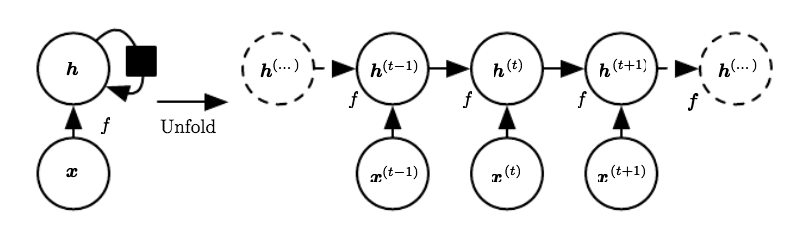
\includegraphics[width=0.9\columnwidth]{rnn.png}
\caption{Grafo de Computação de uma RNN genérica \citep{dlbook}}
\label{fig:rnngraph}
\end{figure}
%%%

Como podemos ver na figura~\ref{fig:rnngraph}, a entrada $x$, ao lado do estado
interno $h$, são usados para calcular um novo estado. 
\\

Essa classe de modelos normalmente é usada para modelagem de linguagem. Buscando
estimar uma distribuição de probabilidade $p(w_t | w_{t-1},w_{t-2},w_{t-3} \dots
) $ onde os $w_i$ são palavras subsequentes de um texto. Normalmente um modelo
dessa natureza busca resolver um problema de classifição, onde a próxima palavra
a ser prevista pelo modelo é uma entre todas as possibilidades de um certo
vocabulário. No caso do domínio em questão desejamamos resolver um problema de
regressão, onde nosso alvo é um valor numérico. Para treinar um desses modelos,
precisamos usar como entrada exemplos subsequentes de dados, onde cada exemplo
de entrada tem um exemplo pareado de saída. Basicamente redes neurais
recorrentes funcionam recebendo um exemplo de entrada, criando uma representação
interna com o mesmo e então gerando uma saída e comparando essa saída com o
exemplo de saída real, gerando um erro. Finalmente, esse erro é propagado para
alterar seus parâmetros (com o fim de achar um conjunto de parâmetros que gere
boas previsões). \\ 


Como já explicado anteriormente, nossos dados de entrada e saída não estão necessariamente pareados perfeitamente dia a dia. Portanto, foi necessário achar intervalos de tempo nos dados onde existe esse pareamento. Isso reduz drasticamente quais períodos representados nos dados realmente podem ser usados para treinar um desses modelos.


\subsubsection{LSTM}

LSTMs \citep{lstm} são um tipo de RNN que por meio de sua arquitetura permitem que sequências
maiores sejam processadas sem que o fluxo dos gradientes propagados pela rede se torne
numericamente problemático (i.e. tendendo a 0 ou a infinito).


\begin{figure}
\centering
\caption{Diagrama da arquitetura de uma LSTM}


\begin{tikzpicture}[
    prod/.style={circle, draw, inner sep=0pt},
    ct/.style={circle, draw, inner sep=5pt, ultra thick, minimum width=10mm},
    ft/.style={circle, draw, minimum width=8mm, inner sep=1pt},
    filter/.style={circle, draw, minimum width=7mm, inner sep=1pt, path picture={\draw[thick, rounded corners] (path picture bounding box.center)--++(65:2mm)--++(0:1mm);
    \draw[thick, rounded corners] (path picture bounding box.center)--++(245:2mm)--++(180:1mm);}},
    mylabel/.style={font=\scriptsize\sffamily},
    >=LaTeX
    ]

\node[ct, label={[mylabel]Cell}] (ct) {$c_t$};
\node[filter, right=of ct] (int1) {};
\node[prod, right=of int1] (x1) {$\times$}; 
\node[right=of x1] (ht) {$h_t$};
\node[prod, left=of ct] (x2) {$\times$}; 
\node[filter, left=of x2] (int2) {};
\node[prod, below=5mm of ct] (x3) {$\times$}; 
\node[ft, below=5mm of x3, label={[mylabel]right:Forget Gate}] (ft) {$f_t$};
\node[ft, above=of x2, label={[mylabel]left:Input Gate}] (it) {$i_t$};
\node[ft, above=of x1, label={[mylabel]left:Output Gate}] (ot) {$o_t$};

\foreach \i/\j in {int2/x2, x2/ct, ct/int1, int1/x1,
            x1/ht, it/x2, ct/it, ct/ot, ot/x1, ft/x3}
    \draw[->] (\i)--(\j);

\draw[->] (ct) to[bend right=45] (ft);

\draw[->] (ct) to[bend right=30] (x3);
\draw[->] (x3) to[bend right=30] (ct);

\node[fit=(int2) (it) (ot) (ft), draw, inner sep=0pt] (fit) {};

\draw[<-] (fit.west|-int2) coordinate (aux)--++(180:7mm) node[left]{$x_t$};
\draw[<-] ([yshift=1mm]aux)--++(135:7mm);
\draw[<-] ([yshift=-1mm]aux)--++(-135:7mm);

\draw[<-] (fit.north-|it) coordinate (aux)--++(90:7mm) node[above]{$x_t$};
\draw[<-] ([xshift=1mm]aux)--++(45:7mm);
\draw[<-] ([xshift=-1mm]aux)--++(135:7mm);

\draw[<-] (fit.north-|ot) coordinate (aux)--++(90:7mm) node[above]{$x_t$};
\draw[<-] ([xshift=1mm]aux)--++(45:7mm);
\draw[<-] ([xshift=-1mm]aux)--++(135:7mm);

\draw[<-] (fit.south-|ft) coordinate (aux)--++(-90:7mm) node[below]{$x_t$};
\draw[<-] ([xshift=1mm]aux)--++(-45:7mm);
\draw[<-] ([xshift=-1mm]aux)--++(-135:7mm);
\end{tikzpicture}


%%% Local Variables:
%%% mode: latex
%%% TeX-master: '../quali'
%%% End:

\label{fig:lstm}
\end{figure}


A figura~\ref{fig:lstm} ilustra o fluxo dos sinais em uma LSTM. \\
Uma rede LSTM possui três \say{portas}. Cada porta possui duas matrizes $W,U$ e um
vetor $b$ de parâmetros. Uma iteração da LSTM começa com o cálculo dos sinais
$o_t,i_t,f_t$.\\

\[f_t = \sigma_g(W_fx_t + U_fh_{t-1} + b_f)\]
\[i_t = \sigma_g(W_ix_t + U_ih_{t-1} + b_i)\]
\[o_t = \sigma_g(W_ox_t + U_oh_{t-1} + b_o)\]

O diferencial de uma LSTM é a propagação do sinal $c_t$, a célula de memória.
Esse valor depende de $f_t$ e $i_t$, que influenciam em como o valor da
célula de memória será atualizado na presente iteração. A equação a seguir
mostra como o valor da célula de memória é calculado. Onde $\circ$ é o produto Hadamard, ou apenas multiplição entrada por entrada de
duas matrizes ou vetores. \\

\[c_t = f_t \circ c_{t-1} + i_t \circ \sigma_c(W_cx_t + U_ch_{t-1} + b_c)\]

Nota-se que $f_t$
define quando de valor antigo da célula de memória deve participar no cálculo do
seu novo valor. 
Da mesma maneira $i_t$ define quanto da nova entrada deve ser usada no cálculo desse valor.
Em outras palavras, as portas $i_t$ e $f_t$ definem o quanto a LSTM deve,
respectivamente, \say{lembrar} e \say{esquecer}.


O novo estado da LSTM é então calculado por: \\
\[h_t = o_t \circ \sigma_h(c_t)\]


\subsubsection{Rede Encoder-Decoder}

Redes Encoder-Decoder são usadas para modelagem de sequência para
sequência, ou seja, para receber dados sequênciais como entrada e gerar
sequências como saída \citep{dlbook}. Esses modelos possuem duas partes, ambas compostas por
RNNs. \\

\begin{figure}[H]
\centering
\begin{tikzpicture}[font=\sffamily]
\node[fill=brown!90!black, text=white, font=\sffamily\small, inner sep=2pt] (a) {\begin{tabular}{@{}r@{}}-0.2\\-0.1\\0.1\\0.4\\-0.3\\1.1\end{tabular}};

\node[fit=(a.north) (a.south), inner sep=1pt, right=1mm of a, minimum width=2cm, label=center:Decoder] (dec) {};
\node[fit=(a.north) (a.south), inner sep=1pt, left=1mm of a, minimum width=2cm, label=center:Encoder] (enc) {};

\begin{scope}[on background layer]
\fill[cyan!30] (dec.north west)--([yshift=5mm]dec.north east)--([yshift=-5mm]dec.south east)--(dec.south west)--cycle;
\fill[cyan!30] (enc.north east)--([yshift=5mm]enc.north west)--([yshift=-5mm]enc.south west)--(enc.south east)--cycle;
\end{scope}

\node[right=1mm of dec, fill=blue, single arrow] (b) {\phantom{a}};
\node[align=left, right=1mm of b] {Sequência de\\ saída};

\node[left=1mm of enc, fill=blue, single arrow] (c) {\phantom{a}};
\node[align=left, left=1mm of c] {Sequência de\\ entrada};
\end{tikzpicture}
%%% Local Variables:
%%% mode: latex
%%% TeX-master: t
%%% End:

\caption{ Diagrama de Rede Encoder-Decoder.\\ Modificado de \cite{encdec}}

\end{figure}
  
O \textbf{encoder} é uma RNN que busca receber uma sequência de entrada de
tamanho arbitrário e gerar uma representação como saída, o seu estado interno,
representando em marrom no diagrama acima. O \textbf{decoder} então recebe essa representação interna (também chamada
de \textit{embedding}) e usa-a para gerar saídas sequencialmente, podendo
então gerar essas sequências de duas formas: O decoder pode usar as suas proprias saídas
como entrada para gerar a saída da próxima iteração temporal, ou então usar dados de treinamento como
entradas, essa última forma chamada de \textit{teacher forcing}. No diagrama
está indicado o embedding entre o decoder e o encoder. Esse embedding é apenas
um vetor (cuja dimensão é um hiper-parâmetro de treinamento) que resume a
informação sequencial lida pelo encoder e a transmite para o decoder. 




\subsubsection{Modelo Encoder-Decoder-Forecaster}

Iremos reproduzir nesse trabalho o modelo proposto em \cite{ubertime}. A
arquitetura consiste em uma rede \textbf{encoder-decoder} que aprende embeddings da
série temporal e então uma rede \textbf{forecaster} que usa esses embeddings ao lado de
variáveis exógenas a série temporal para realizar predições.  


\begin{figure}[H]
\centering
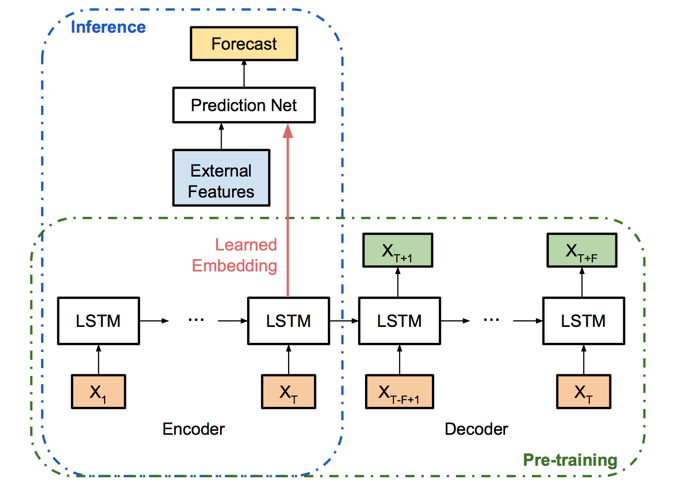
\includegraphics[width=0.9\columnwidth]{uber.png}
\caption{Arquitetura do modelo proposto por \cite{ubertime}}
\end{figure}


Durante o pré-treinamento a rede encoder-decoder consome sequências de $F$ dias
da série temporal. O encoder cria uma representação vetorial $h$ depois de
receber como entrada os primeiros $T$ ($T < F$) dias da sequência. Então, $h$ é usado como
inicialização do estado interno do decoder, e esse então consume mais $F - T$
entradas da sequência. Para o decoder, se em uma iteração sua entrada é $X_i$,
então sua saída será comparada com $X_{i+1}$, e esse erro é propagado após lidas
todas as entradas para que a representação $h$ proveniente do encoder possa se
tornar mais informativa.


Esse modelo também possui outra característica importante. Todas as camadas da
redes neurais que compõe o encoder, o decoder e o forecaster possuem
Dropout com probabilidade $p$. Ou seja, podemos usar a técnica do Monte
Carlo Dropout para estimar a variância de cada predição feita por esse modelo. \\










%%% Local Variables:
%%% mode: latex
%%% TeX-master: "../quali"
%%% bibtex-file-path: "../bibliografia"
%%% End:
\par


\chapter{Estudo dos Dados}
\label{cap:estudodados}


\section{Preparo dos Dados}

\subsection{Contagem de dias válidos}

Para treinar algum tipo de modelo preditivo com os dados, é necessário parear dados de entrada e de saída. Para os diversos conjuntos de dados cedidos pela Intercement, os mesmos representam diferentes momentos da produção de cimento. Então ao usarmos algum desses dados como entrada para prever uma saída, devemos adicionar o delay temporal correspondente ao tempo que demora para entrada se tornar saída. Por exemplo, se tentarmos prever os dados de expedição com os dados de farinha, o delay apropriado é de 10 dias. No restante desse documento esse delay sempre foi considerado independente de quais dados estejam sendo usados.

Também devemos notar o fato que a frequência na qual os dados de Clínquer, Farinha e Cimento Cru são anotados é bastante maior que a frequência temporal dos dados de expedição. O que também dificulta o pareamento. Por exemplo, temos dados de Clínquer a cada hora, sendo que os dados de expedição são anotados dia a dia. Portanto, foi necessário unir dados de um mesmo dia (tirando a média das suas entradas) para que fosse possível associar diferentes conjuntos de dados de um para um.
\begin{enumerate}
    \item Os dados de  Clínquer possuem 3528 linhas de dados de 2936 dias distintos
\item Os dados de  Expedição possuem 3650 linhas de dados de 2520 dias distintos
\item Os dados de  Farinha possuem 3530 linhas de dados de 2937 dias distintos
\item Os dados de  Cru possuem 30558 linhas de dados de 30558 dias distintos
\end{enumerate}

\subsection{Dados faltantes}
Embora tenhamos uma quantidade razoável de dias com dados presentes, esses muitas vezes não possuem alguma de suas colunas.
A seguir vemos para todos os dataframes, para cada uma de suas colunas, quantos dias possuem dados faltantes.



\captionof{table}{Dias com dados faltantes para cada parâmetro de Clínquer}
\begin{center}
\begin{tabular}{ c c }
 CaOL       &      596\\
Fe2O3       &    596\\
CaO         &   596\\
SiO2        &  596\\
Al2O3       & 596\\
P2O5        & 596\\
MgO         & 596\\
K2O         & 596\\
Na2O        & 596\\
CLOR        & 2724\\
FLUOR       & 2095\\
MS          & 596\\
MA          & 596\\
FSC         & 596\\
RSA         & 809\\
C3S         & 596\\
C2S         & 596\\
C3A         & 596\\
C4AF        & 596\\
F.liq       & 596\\
25,4 mm     & 2753\\
12,7 mm     & 2752\\
6,35  mm    & 2752\\
3,36 mm     & 2752\\
\textless 3,36 mm    & 2756
\end{tabular}
\end{center}
\newpage
\captionof{table}{Dias com dados faltantes para cada parâmetro de Expedição}
\begin{center}
\begin{tabular}{ c c }
AGP     &  1131\\
IP      &  1131\\
FP      &  1132\\
G75    &  1133\\
G44   &  1153\\
MVOL    &  1656\\
SBL     &  1131\\
RC3     &  1130\\
RC7     &  1130\\
RC28    &  1130\\
RICARB  &  1331\\
PF      &  1136\\
AL2O3   &  1140\\
CAOT    &  1140\\
K2O     &  1140\\
MGO     &  1139\\
SIO2    &  1140\\
FE2O3   &  1140\\
SO3     &  1137\\
NA2O    &  3139\\
P2O5    &  1141\\
EXP     &  2804\\
RC1     &  1861\\
RC91    &  3638\\
CO2     &  3629 
\end{tabular}
\end{center}

\newpage

\captionof{table}{Dias com dados faltantes para cada parâmetro de Farinha}
\begin{center}
\begin{tabular}{ c c }
Fe2O3     &   595\\
CaO       &  595\\
SiO2      &   595\\
Al2O3     &   595\\
SO3       &   595\\
P2O5      &   595\\
MgO       &   595\\
K2O       &   595\\
Na2O      &   931\\
CLOR.     &  1697\\
FLUOR.    &  1588\\
FSC       &   595\\
MS        &   595\\
MA        &   595\\
RSA       &   815\\
P. F AL.  &   593 \\
\end{tabular}
\end{center}

\newpage

\captionof{table}{Dias com dados faltantes para cada parâmetro de Cimento Cru}
\begin{center}
\begin{tabular}{ c c }
Alim. (t/h)       & 131\\
Prod (ton)        & 250\\
Calc. (\%)        & 131\\
Arg. (\%)         & 131\\
Areia (\%)        & 132\\
Corr. (\%)        & 370\\
Caulim (\%)       & 421\\
Cinza (\%)        & 295\\
Alurox (\%)       & 442\\
Fe2O3             & 44\\
CaO               & 44\\
SiO2              & 44\\
Al2O3             & 44\\
SO3               & 44\\
P2O5              & 44\\
MgO              &  44\\
K2O              &  44\\
Na2O             &  48\\
MA               &  44\\
MS               &  44\\
FSC              &  44\\
\#100             & 187\\
\#170             &  44\\
Umid Calc (\%)   &  413\\
Umid Arg (\%)    &  414 \\
Umid Areia (\%) &    391 \\
\end{tabular}
\end{center}




\subsection{Resample dos dados}
Para maior facilidade de manuseio dos dados. Foi necessário realizar um \textbf{resample}. Os dados foram modificados para que entradas realizadas no mesmo dia sejam unificadas. E dias sem dados foram criados como placeholders para facilidade de vizualiação dos dados. A seguir são reproduzidas as contagens de dados após o resample.


\begin{itemize}
\item Clínquer: Temos dados de entrada do dia 22/04/2008 até o dia 18/12/2017
\item Clínquer: De um período de 3528 dias temos 2932 dias preenchidos com dados de entrada
\item Expedição: Temos dados de entrada do dia 02/01/2008 até o dia 29/12/2017
\item Expedição: De um período de 3650 dias temos 2520 dias preenchidos com dados de entrada
\item Farinha: Temos dados de entrada do dia 20/04/2008 até o dia 18/12/2017
\item Farinha: De um período de 3530 dias temos 2937 dias preenchidos com dados de entrada
\item Cru: Temos dados de entrada do dia 21/04/2008 até o dia 09/12/2016
\item Cru: De um período de 3155 dias temos 2675 dias preenchidos com dados de entrada
\end{itemize}


\section{Testes de Sazonalidade}

Diversas publicações recentes estudam a eficácia de modelos de Deep Learning para predição de séries temporais, como consumo de energia elétrica. Os dados estudados nesse documento são séries temporais dado que são indexados pelo tempo, porém, resta analisar características temporais desses dados. No exemplo do consumo de energia elétrica, poderiamos notar que, ao longo de vários anos presentes nos dados, o consumo de energia de uma certa residência aumenta em determinado mês. Isso seria um fator útil que um modelo poderia aprender para a predição futura do consumo dessa residência. Dados que não possuem nenhuma característica temporal (i.e. a ordem não importa) seriam por exemplo provenientes de um estudo do salário recebido por uma amostra da população dados fatores como gênero, escolaridade e idade. No primeiro exemplo temos um caso de \textbf{sazonalidade} nos dados, algo que pode ser analisado em séries temporais com testes de análise espectral e auto-correlação. Para os dados desse problema, iremos testar a sazonalidade dos preditores de dureza do cimento.

\subsection{Análise Espectral}

Uma maneira de testar sazonalidade de dados indexados temporalmente é usar a técnica de Transformada de Fourier, onde podemos estudar quais frequencias dentro de um espectro podem ser usadas para decompor um sinal (i.e. nossos dados). Para essa análise usamos os índices de dureza contidos nos dados de expedição, de 2008 até 2014 e descartamos a parte imaginária da análise já que nossos dados não possuem parte complexa. Seguem os resultados:


\begin{figure}[H]
\centering
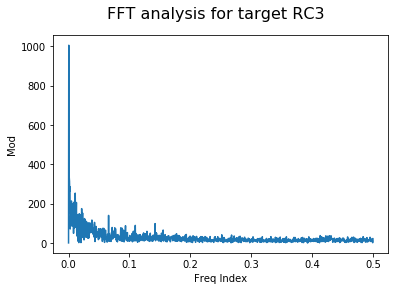
\includegraphics[width=0.9\columnwidth]{FFT_RC3.png}
\caption{Análise Espectral para preditor RC3}
\end{figure}

\begin{figure}[H]
\centering
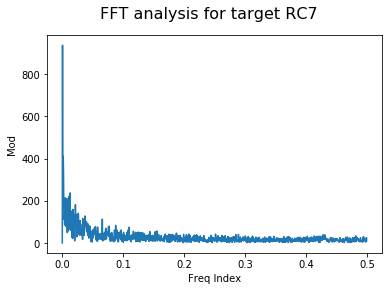
\includegraphics[width=0.9\columnwidth]{FFT_RC7.png}
\caption{Análise Espectral para preditor RC7}
\end{figure}

\begin{figure}[H]
\centering
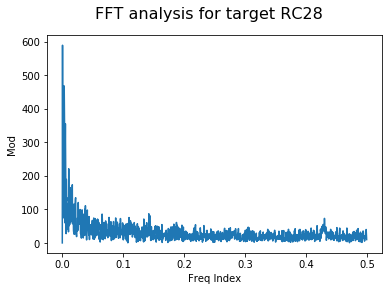
\includegraphics[width=0.9\columnwidth]{FFT_RC28.png}
\caption{Análise Espectral para preditor RC28}
\end{figure}


Podemos notar que a "energia" do sinal não possui picos em nenhuma frequência além da frequência zero, que seria a potência média do sinal, ou seja, uma componente que não depende do tempo. Então, afirmamos que esses dados não possuem sazonalidade mensal ou anual. O que significa que a média e a variância desses indicadores não possuem trends e.g. alguma mudança similar todo mês de Janeiro.



\par

\chapter{Resultados Experimentais }
\label{cap:resultados}

\section{Resultados}


Todos os testes foram feitos com normalização min-max dos dados, para que se evite comportamentos estranhos por parte das redes neurais. \\

\bigskip

Como teste da acurácia dos modelos foi usada a métrica R-quadrado. Sejam $\hat{y}$ e $y$ nossa previsão dada pelo modelo e o seu valor real, a acurácia do modelo é dada por:\\

\bigskip

\begin{center}
$R_2 = 1 - \frac{SS_{res}}{SS_{tot}}$\\

$SS_{tot} = \sum (y - \hat{y})^2$

$SS_{res} = \sum (y - \bar{y})^2$

$  \bar{y} = \frac{1}{n} \sum y$
\end{center}
\bigskip

%\justify
Para essa métrica, o modelo pode performar arbitrariamente mal, com esse valor podendo se tornar arbitrariamente negativo. Porém, seu valor máximo é 1, indicando um modelo ideal.\\

\bigskip
\subsection{Primeiro Ensaio}
A seguir são reproduzidos gráficos de um experimento realizado com o fim de comparar nossos modelos. Usamos os dados de Farinha para prever os índices RC3, RC7 e RC28. Foi preferido treinar um modelo de cada tipo para cada um dos índices, por simplicidade. Ou seja, são usados parâmetros dos dados de entrada com o fim de prever um único parâmetro de saída. //
Para o treinamento e teste de cada modelo, separamos os dados em duas partes. Nesse experimento os dados de farinha e expedição de 2008 a 2016 foram usados como dados de treinamento e 30\% desses foram aleatóriamente selecionados para servirem de dados de teste, chamado no jargão técnico como \textit{test set}. Finalmente, os dados de 2017 e 2018 foram usados como um segundo conjunto de dados de treinamento, estes em um período completamente inédito para os modelos treinados, esse segundo conjunto chamado por sua vez usualmente de \textit{dev set}. Os gráficos a seguir mostram em azul os dados reais de 2017 em diante, bem como as previsões feitas por cada modelo em laranja. As métricas R-quadrado para cada conjunto de dados de teste também são mostradas no canto inferior direito.



\begin{figure}[H]
\centering
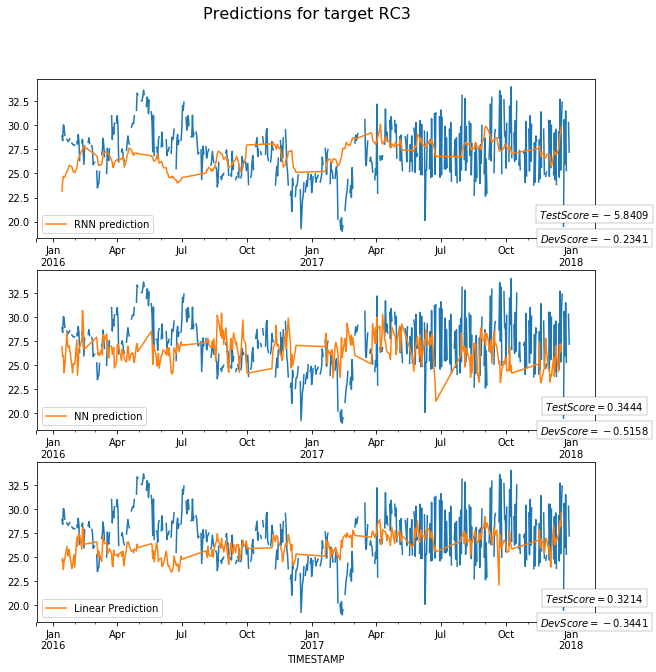
\includegraphics[width=0.9\columnwidth]{RC3.png}
\caption{Comparação dos 3 modelos na tarefa de regressão do índice RC3}
\end{figure}

\begin{figure}[H]
\centering
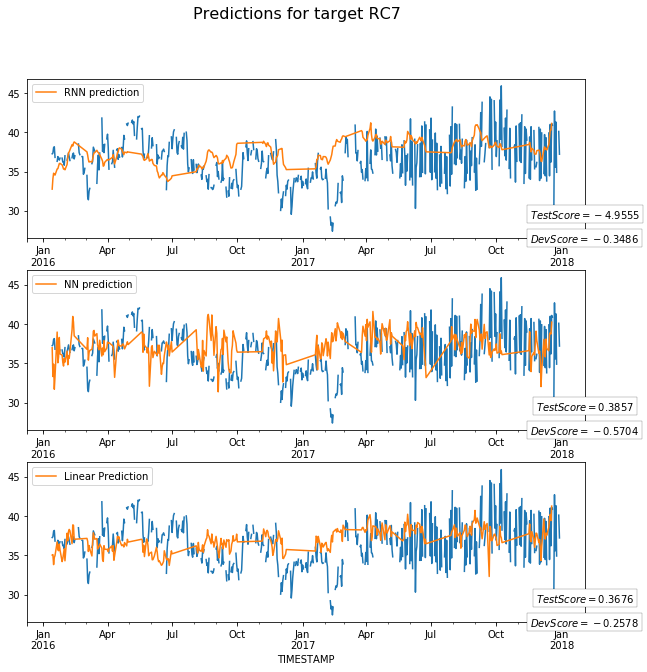
\includegraphics[width=0.9\columnwidth]{RC7.png}
\caption{Comparação dos 3 modelos na tarefa de regressão do índice RC7}
\end{figure}

\begin{figure}[H]
\centering
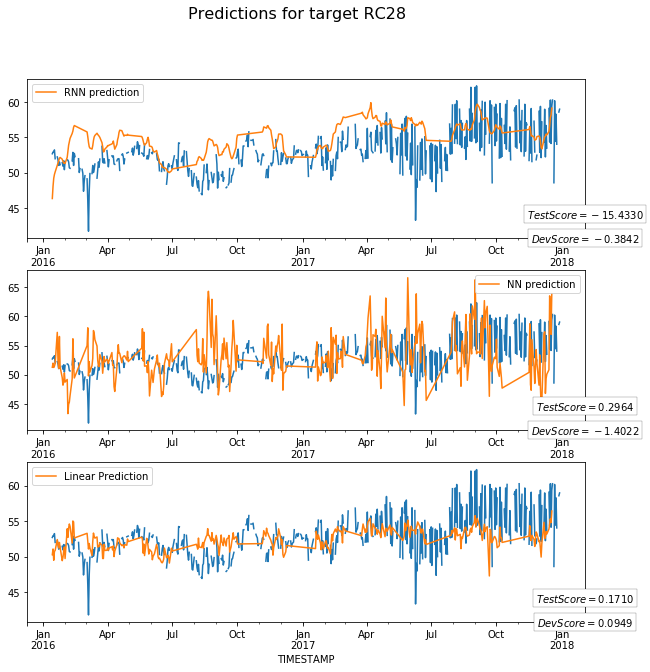
\includegraphics[width=0.9\columnwidth]{RC28.png}
\caption{Comparação dos 3 modelos na tarefa de regressão do índice RC28}
\end{figure}


\subsection{Segundo Ensaio}

Estudando os dados vemos que ouve um aumento repentino dos índices de dureza a partir de 2016, e um ruído sensivelmente mais presente e com uma variância maior. Várias tentativas foram feitas com diversos parâmetros de entrada e nenhum conjunto destes ajuda a prever essa mudança brusca nos dados. Portanto devemos concluir que ela é dada por fatores não presentes nos dados concedidos. O primeiro ensaio foi realizado com os dados de treinamento sendo de 2008 a 2015, com o restante sendo nossos dados de validação. Uma performance melhor possivelmente seria atingida se usarmos dados antes de 2016 para treinamento e validação. //


Segue um plot da nova divisão dos dados entre treino/teste e validação para os índices que estamos tentando modelar:

\begin{figure}[H]
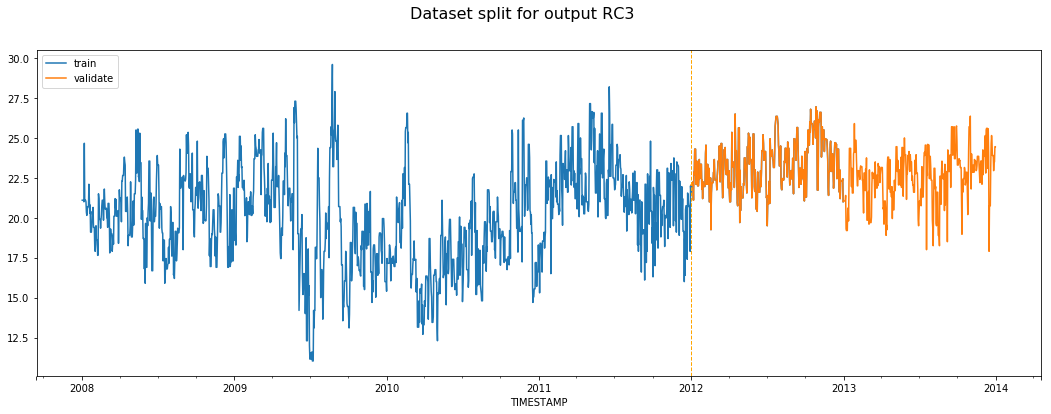
\includegraphics[width=0.9\columnwidth]{dataset_splitRC3.png}
\caption{Divisão do dataset para a saída RC3}
\end{figure}

\begin{figure}[H]
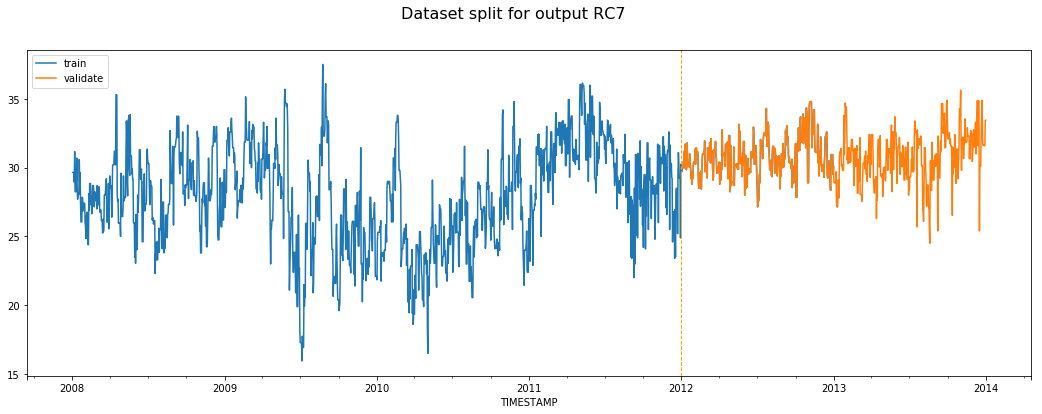
\includegraphics[width=0.9\columnwidth]{dataset_splitRC7.png}
\caption{Divisão do dataset para a saída RC7}
\end{figure}

\begin{figure}[H]
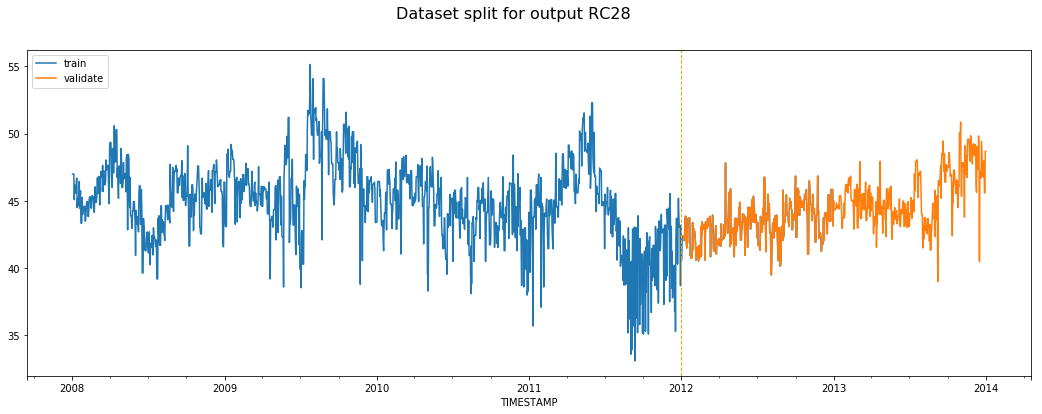
\includegraphics[width=0.9\columnwidth]{dataset_splitRC28.png}
\caption{Divisão do dataset para a saída RC28}
\end{figure}


Finalmente, seguem plots dos novos resultados, esses sendo reproduzidos apenas para o período inédito para os modelos, ou seja, o \textbf{dev set} de 2012 até 2014:


\bigskip
Primeiro, os modelos considerando os dados como não-sequenciais:

\begin{figure}[H]
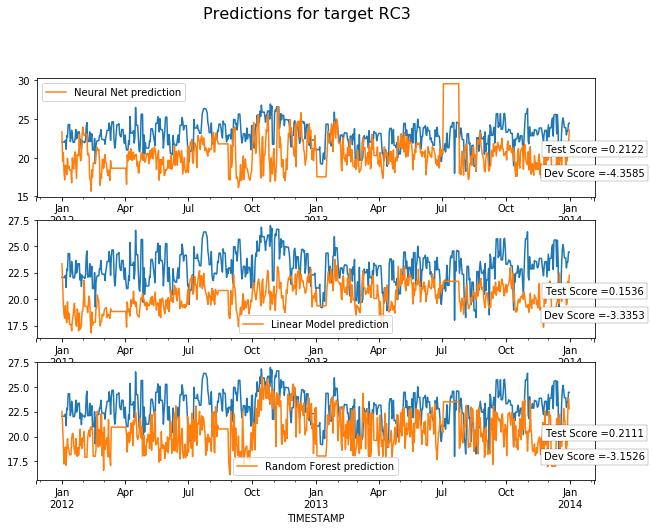
\includegraphics[width=0.9\columnwidth]{farinha_2008-2012-2014RC3.png}
\caption{Comparação dos 3 modelos não-sequenciais na tarefa de regressão do índice RC3}
\end{figure}

\begin{figure}[H]
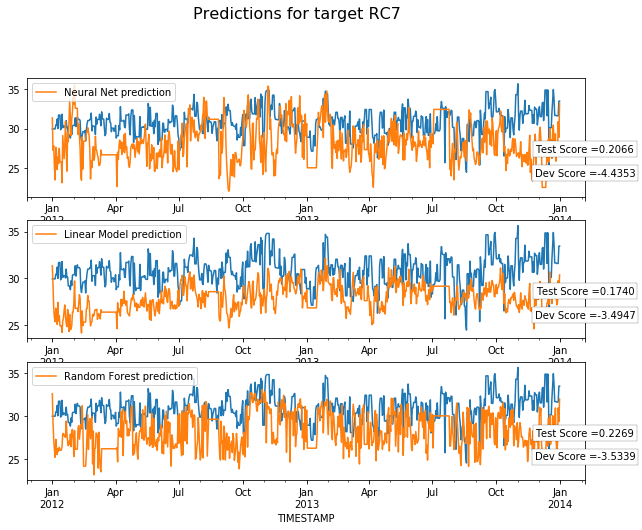
\includegraphics[width=0.9\columnwidth]{farinha_2008-2012-2014RC7.png}
\caption{Comparação dos 3 modelos não-sequenciais na tarefa de regressão do índice RC7}
\end{figure}

\begin{figure}[H]
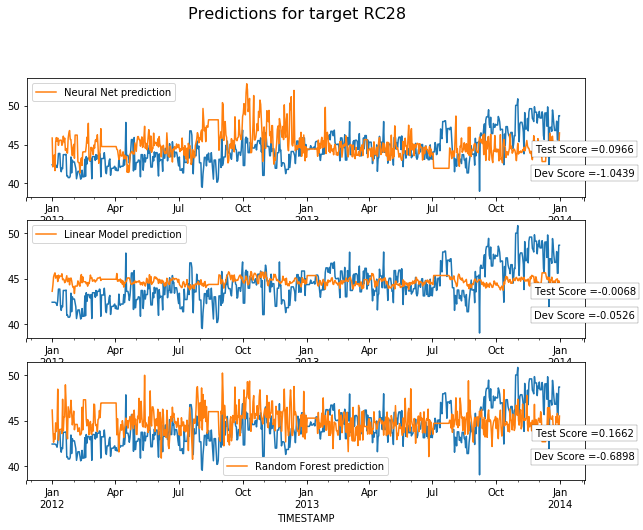
\includegraphics[width=0.9\columnwidth]{farinha_2008-2012-2014RC28.png}
\caption{Comparação dos 3 modelos não-sequenciais na tarefa de regressão do índice RC28}
\end{figure}


Agora, a performance da Rede Neural usando a técnica de Monte Carlo Dropout para inferência Bayesiana e cálculo de incerteza:


\begin{figure}[H]
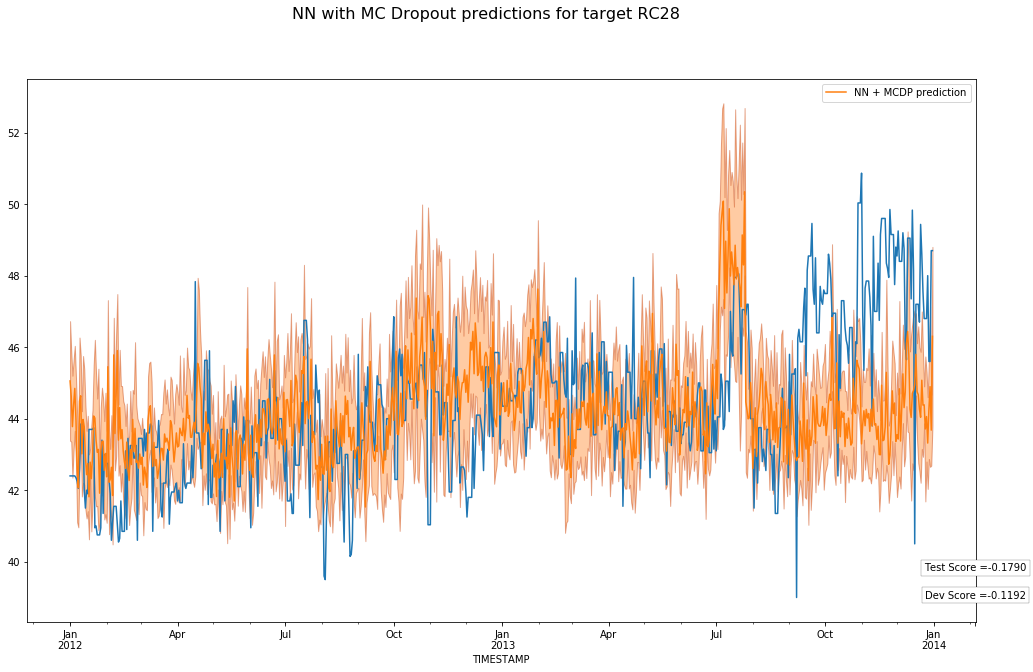
\includegraphics[width=1\columnwidth]{NNMCDP_2012-2014RC28.png}
\caption{Performance do modelo Rede Neural + MC Dropout para o índice RC28}
\end{figure}


É interessante notar que o modelo anterior com a sua capacidade de calcular incertezas, realiza uma boa tarefa de  ''cobrir'' os dados reais com a sua incerteza prevista para os pontos de dados previstos. \\ 

Finalmente, temos o modelo de Rede Neural Recorrente, um modelo sequencial:


\begin{figure}[H]
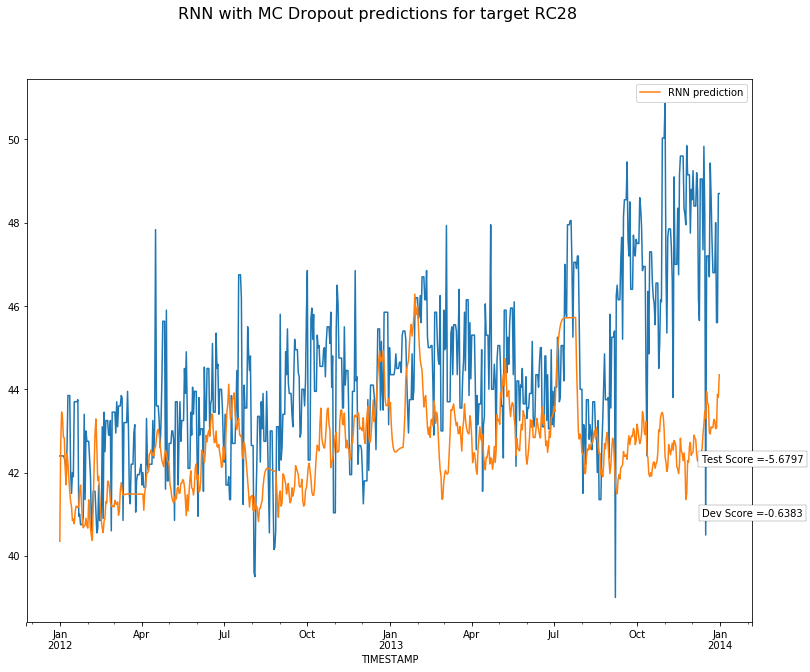
\includegraphics[width=0.9\columnwidth]{RNN_2012-2014RC28.png}
\caption{Performance do modelo RNN para o índice RC28}
\end{figure}


\bigskip

Dos resultados obtidos podemos perceber que a acurácia dos modelos aumenta sensivalmente para o índice RC28, isso se dá pelo fato que essa é uma medida na qual naturalmente está envolvido menos ruído e incerteza que as outras duas. Analisando os valores da métrica R2, os melhores modelos atingiram valores próximos de $0$.


\par

%% ------------------------------------------------------------------------- %%
\chapter{Conclusões}
\label{cap:conclusoes}


Pelos resultados obtidos, é possível concluir que não houveram ganhos
significativos em usarmos modelos sequenciais de Deep Learning na modelagem dos
dados. Como uma simples regressão linear consegue em alguns casos uma
performance até melhor que uma rede neural ou uma rede recorrente, podemos afirmar também que a natureza temporal dos dados não é útil na modelagem dos mesmos. A performance de modelos que consideram esses dados não-sequenciais obteve uma performance equivalente ou melhor.

Os dados possuem uma grande quantidade de ruído proveniente de incertezas no instante das medições, o que dificulta o aprendizado seja de qual modelo for usado. E também é claro que ao longo dos 10 anos de dados possuimos mudanças bruscas de valores provenientes de fatores não presentes nos dados. Ou seja, do domínio que queremos aprender temos dados com um ruído alto e variável além de não possuirmos toda a informação do suposto "processo gerador de dados" (a distribuição de probabilidades $p$ que queremos estimar), o que dificulta qualquer modelo estatístico para o qual iremos dar essa tarefa.

Como uma regressão linear consegue resultados comparáveis a modelos diferentes e mais complexos, pode-se afirmar que a distribuição de probabilidade que queremos estimar para os preditores não é muito complexa, mas os fatores mencionados no parágrafo anterior atrapalham uma melhor performance dos modelos usados. Resultados melhores possivelmente podem ser obtidos usando métodos clássicos de Machine Learning como \textbf{feature engineering}, ou seja, aplicar um conhecimento específico do domínio do problema em questão para deixar menos para os modelos decidirem sozinhos. O que é imcompatível com métodos de Deep Learning. 




\section{Cronograma de Pesquisa}


\begin{figure}[H]
\begin{center}
     \begin{ganttchart}[%Specs
     y unit title=0.5cm,
     y unit chart=0.7cm,
     vgrid,hgrid,
     title height=1,
%     title/.style={fill=none},
     title label font=\bfseries\footnotesize,
     bar/.style={fill=blue},
     bar height=0.7,
%   progress label text={},
     group right shift=0,
     group top shift=0.7,
     group height=.3,
     group peaks width={0.2},
     inline]{1}{24}
     % labels


     % Titulo da tabela e quantos quadradinhos vai ter no total
     \gantttitle{2018-2019 - Mestrado}{24}\\

     % primeira subdivisão de quadradinhos em anos, quantos quadradinhos tem por
     % ano(precisa somar o mesmo que o valor
     % que vc definiu em cima)
    \gantttitle[]{2018}{12}                 
    \gantttitle[]{2019}{12} \\              

    %% subsubdivisão de quadradinhos em meses, tb precisa somar o total
    %% desse jeito cada quadradinho conta como 1 semana de trabalho
    %% 4 quadradinhos por mes
    \gantttitle{Outubro}{4}                
    \gantttitle{Novembro}{4}
    \gantttitle{Dezembro}{4}
    \gantttitle{Janeiro}{4}
    \gantttitle{Fevereiro}{4}
    \gantttitle{Março}{4}\\


    %%% primeiro valor nos colchetes -> nome da tarefa
    %% segundo e terceiro valores -> de qual quadradinho até qual quadradinho a
    %% tarefa vai, de acordo com o numero de quadradinhos que vc definiu la em
    %% cima
    \ganttbar[inline=false]{Tarefa 1}{1}{4}\\
    \ganttbar[inline=false]{Tarefa 2}{2}{6}\\ 
    \ganttbar[inline=false]{Tarefa 3}{3}{8} \\
    \ganttbar[inline=false]{Tarefa 4}{5}{10} \\
    \ganttbar[inline=false]{Tarefa 5}{8}{12} \\
    \ganttbar[inline=false]{Tarefa 6}{12}{20} \\
    \ganttbar[inline=false]{Tarefa 7}{13}{21} \\
    \ganttbar[inline=false]{Tarefa 8}{14}{24} \\



    
\end{ganttchart}
\end{center}
\caption{Cronograma dos próximos passos de Pesquisa}
\end{figure}

\begin{itemize}

\item[Tarefa 1: ] Refazer Experimentos sem o delay temporal, apenas com os dados
  de Expedição de Cimento
\item[Tarefa 2: ] Usar modelo para outros dados de séries temporais (e.g. clima)
\item[Tarefa 3: ] Nova compilação de resultados
\item[Tarefa 4: ] Uso de dados de outras etapas da produção de concreto simultaneamente
\item[Tarefa 5: ] Estudar alterações no modelo proposto pela Uber  
\item[Tarefa 6: ] Experimentos com mudanças propostas 
\item[Tarefa 7: ] Estudo e compilação de resultados
\item[Tarefa 8: ] Escrita da tese 


  
\end{itemize}

% ------------------------------------------------------
%% 
%% \section{Considerações Finais} 
%% 
%% Texto texto texto texto texto texto texto texto texto texto texto texto texto
%% texto texto texto texto texto texto texto texto texto texto texto texto texto
%% texto texto texto texto texto texto. 
%% 
%% %------------------------------------------------------
%% \section{Sugestões para Pesquisas Futuras} 
%% 
%% Texto texto texto texto texto texto texto texto texto texto texto texto texto
%% texto texto texto texto texto texto texto texto texto texto texto texto texto
%% texto texto texto texto texto texto.

%%% Local Variables:
%%% mode: latex
%%% TeX-master: "../quali"
%%% bibtex-file-path: "../bibliografia"
%%% End:
\par

\par


%%%%%%%%%%%%%%%%%%%%%%%%%%%%%%%% APÊNDICES %%%%%%%%%%%%%%%%%%%%%%%%%%%%%%%%%%%%%

% Aqui vão apêndices. O comando appendix reinicia a numeração de capítulos e
% passa a numerá-los com letras. Como os anteriores, ele não existe na classe
% "article".
\appendix

% Este formato está definido mais acima na seção "APARÊNCIA/FORMATAÇÃO"
\pagestyle{appendix}

% Os apêndices podem ser inseridos diretamente aqui ou "puxados" de outros
% arquivos


\chapter{Tabelas dos demais dados}
\label{ape:tables}

\captionof{table}{Dias com dados faltantes para cada parâmetro de Farinha}
\begin{center}
\begin{tabular}{ c c }
Fe2O3     &   595\\
CaO       &  595\\
SiO2      &   595\\
Al2O3     &   595\\
SO3       &   595\\
P2O5      &   595\\
MgO       &   595\\
K2O       &   595\\
Na2O      &   931\\
CLOR.     &  1697\\
FLUOR.    &  1588\\
FSC       &   595\\
MS        &   595\\
MA        &   595\\
RSA       &   815\\
P. F AL.  &   593 \\
\end{tabular}
\end{center}

\newpage
\captionof{table}{Dias com dados faltantes para cada parâmetro de Cimento Cru}
\begin{center}
\begin{tabular}{ c c }
Alim. (t/h)       & 131\\
Prod (ton)        & 250\\
Calc. (\%)        & 131\\
Arg. (\%)         & 131\\
Areia (\%)        & 132\\
Corr. (\%)        & 370\\
Caulim (\%)       & 421\\
Cinza (\%)        & 295\\
Alurox (\%)       & 442\\
Fe2O3             & 44\\
CaO               & 44\\
SiO2              & 44\\
Al2O3             & 44\\
SO3               & 44\\
P2O5              & 44\\
MgO              &  44\\
K2O              &  44\\
Na2O             &  48\\
MA               &  44\\
MS               &  44\\
FSC              &  44\\
\#100             & 187\\
\#170             &  44\\
Umid Calc (\%)   &  413\\
Umid Arg (\%)    &  414 \\
Umid Areia (\%) &    391 \\
\end{tabular}
\end{center}

\newpage
\captionof{table}{Dias com dados faltantes para cada parâmetro de Clínquer}
\begin{center}
\begin{tabular}{ c c }
 CaOL       &      596\\
Fe2O3       &    596\\
CaO         &   596\\
SiO2        &  596\\
Al2O3       & 596\\
P2O5        & 596\\
MgO         & 596\\
K2O         & 596\\
Na2O        & 596\\
CLOR        & 2724\\
FLUOR       & 2095\\
MS          & 596\\
MA          & 596\\
FSC         & 596\\
RSA         & 809\\
C3S         & 596\\
C2S         & 596\\
C3A         & 596\\
C4AF        & 596\\
F.liq       & 596\\
25,4 mm     & 2753\\
12,7 mm     & 2752\\
6,35  mm    & 2752\\
3,36 mm     & 2752\\
\textless 3,36 mm    & 2756
\end{tabular}
\end{center}

\chapter{Gráficos dos demais índices testados}
\label{ape:graphs}


\begin{figure}[H]
\centering
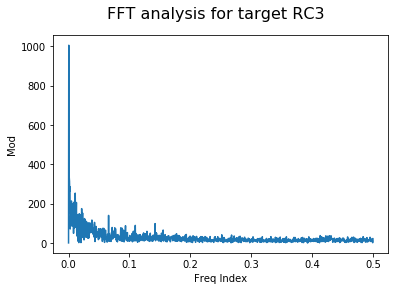
\includegraphics[width=0.9\columnwidth]{FFT_RC3.png}
\caption{Análise Espectral para preditor RC3}
\end{figure}

\begin{figure}[H]
\centering
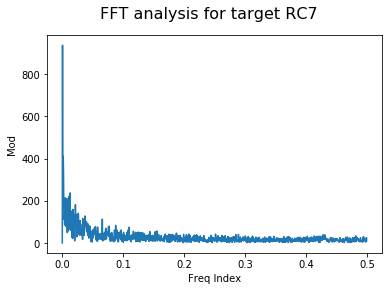
\includegraphics[width=0.9\columnwidth]{FFT_RC7.png}
\caption{Análise Espectral para preditor RC7}
\end{figure}

\begin{figure}[H]
\centering
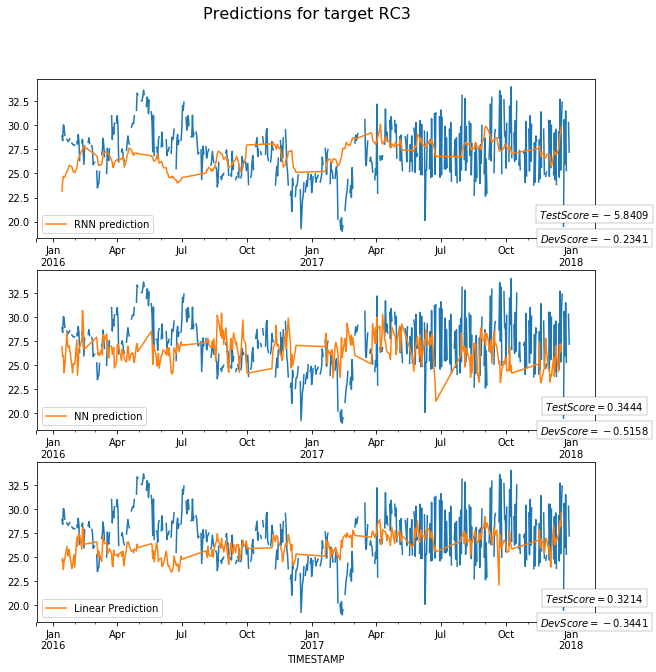
\includegraphics[width=0.9\columnwidth]{RC3.png}
\caption{Comparação dos 3 modelos não-sequenciais na tarefa de regressão do índice RC3}
\end{figure}

\begin{figure}[H]
\centering
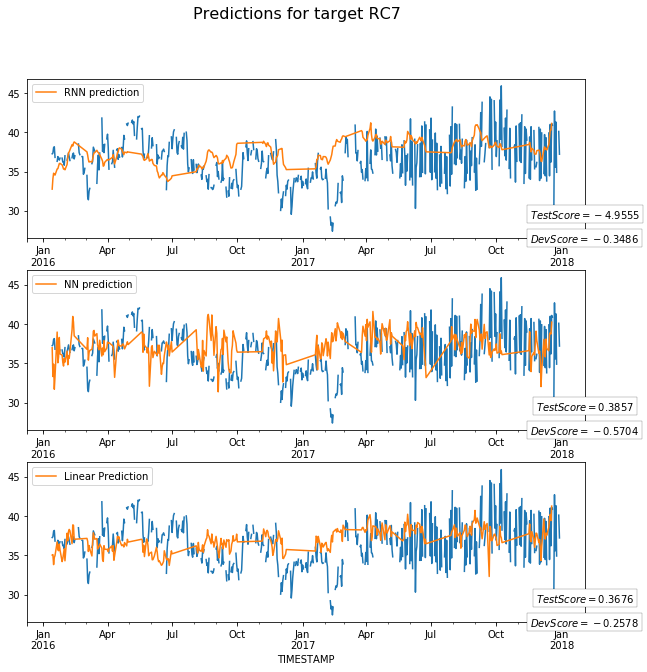
\includegraphics[width=0.9\columnwidth]{RC7.png}
\caption{Comparação dos 3 modelos não-sequenciais na tarefa de regressão do índice RC7}
\end{figure}

\begin{figure}[H]
\centering
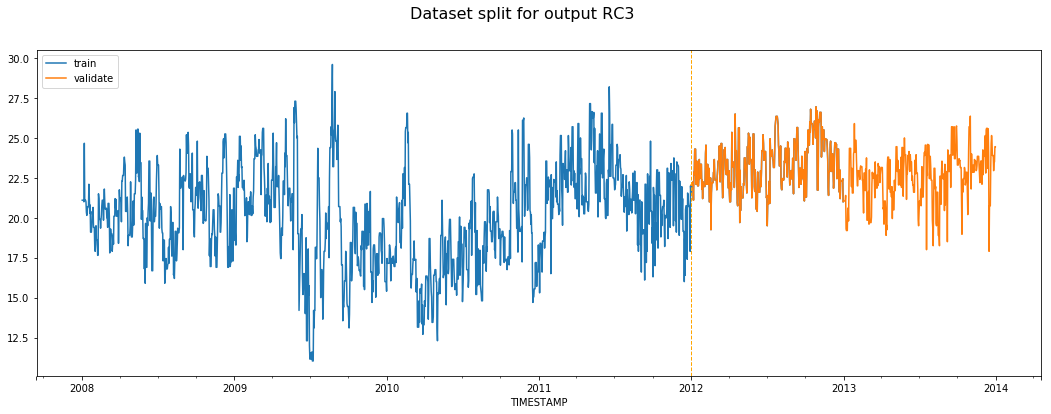
\includegraphics[width=0.9\columnwidth]{dataset_splitRC3.png}
\caption{Divisão do dataset no segundo ensaio para a saída RC3}
\end{figure}

\begin{figure}[H]
\centering
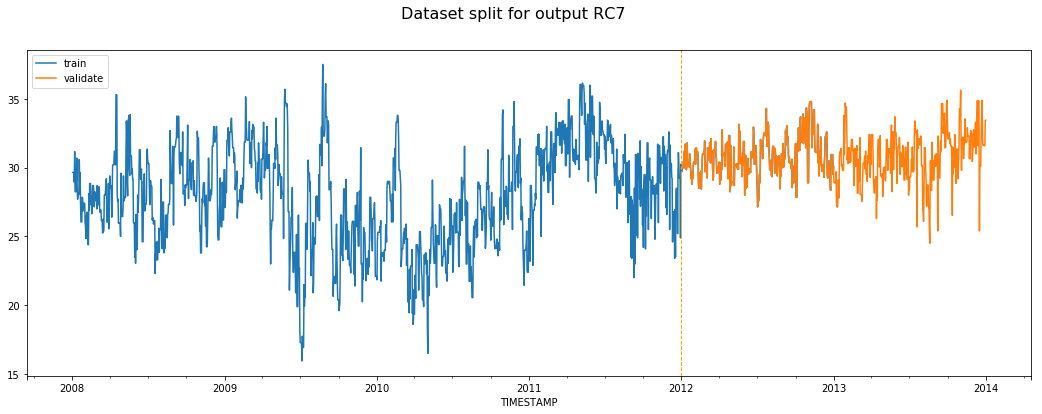
\includegraphics[width=0.9\columnwidth]{dataset_splitRC7.png}
\caption{Divisão do dataset no segundo ensaio para a saída RC7}
\end{figure}

\begin{figure}[H]
\centering
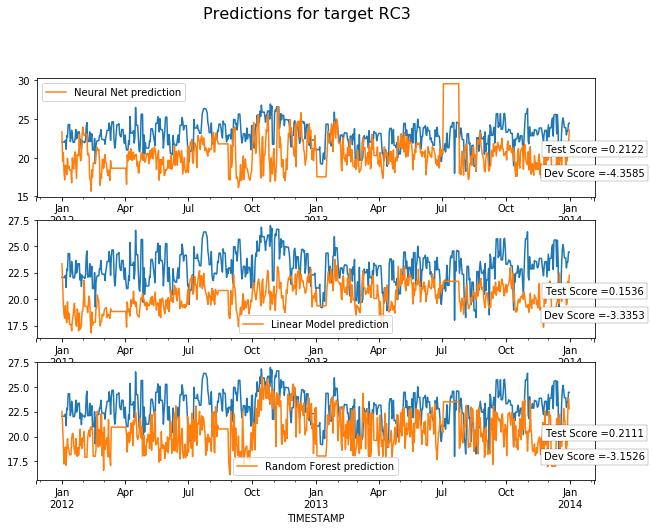
\includegraphics[width=0.9\columnwidth]{farinha_2008-2012-2014RC3.png}
\caption{Comparação dos 3 modelos não-sequenciais na tarefa de regressão do índice RC3}
\end{figure}

\begin{figure}[H]
\centering
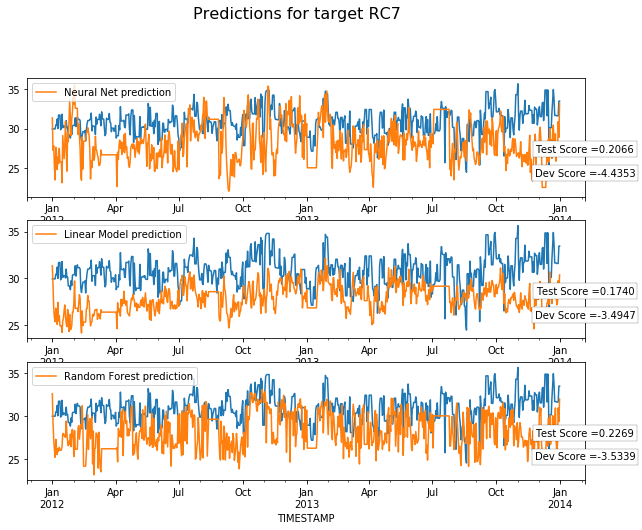
\includegraphics[width=0.9\columnwidth]{farinha_2008-2012-2014RC7.png}
\caption{Comparação dos 3 modelos não-sequenciais na tarefa de regressão do índice RC7}
\end{figure}


\par


%%%%%%%%%%%%%%%%%%%%%%%%%%%%%% SEÇÕES FINAIS %%%%%%%%%%%%%%%%%%%%%%%%%%%%%%%%%%%

% Aqui vão a bibliografia, índice remissivo e outras seções similares.
% O comando backmatter desabilita a numeração de capítulos e também não existe
% na classe "article".
\backmatter

% Este formato está definido mais acima na seção "APARÊNCIA/FORMATAÇÃO"
\pagestyle{frontback}

\singlespacing   % espaçamento simples

% A bibliografia é obrigatória

%%%%%%%%% Bibliografia com natbib (preterido): %%%%%%%%%
%\bibliographystyle{alpha-ime}% citação bibliográfica alpha
%\bibliographystyle{plainnat-ime} % citação bibliográfica textual
%\bibliography{bibliografia}  % associado ao arquivo: 'bibliografia.bib'

%%%%%%%% Bibliografia com biblatex (preferido): %%%%%%%%

\printbibliography[
  title=Bibliografia\label{bibliografia},
  % Inclui a bibliografia no sumário; comente se estiver usando "article"
  heading=bibintoc,
]

% imprime o índice remissivo no documento (opcional)
\printindex

\end{document}
